% !TeX root = ../main.tex
\documentclass[./../main.tex]{subfiles}

\begin{document}

Phần này mô tả sản phẩm cuối sau quá trình phát triển của em, bao gồm
hình ảnh của giao diện người dùng thuộc phần client. Phần giao diện
người dùng sẽ được bạn Phạm Thị Dân mô tả kỹ hơn ở một báo cáo khác.

\subsection{Luồng sử dụng của sinh viên}

\paragraph*{Sinh viên đọc bài đăng}

\begin{itemize}
\item Hình \ref{fig:student_home_page}: Sinh viên truy cập trang chủ và chọn bài đăng muốn đọc.
\item Hình \ref{fig:student_read_post_page}: Giao diện hiển thị bài đăng đã chọn.
\end{itemize}

\begin{figure}[]
	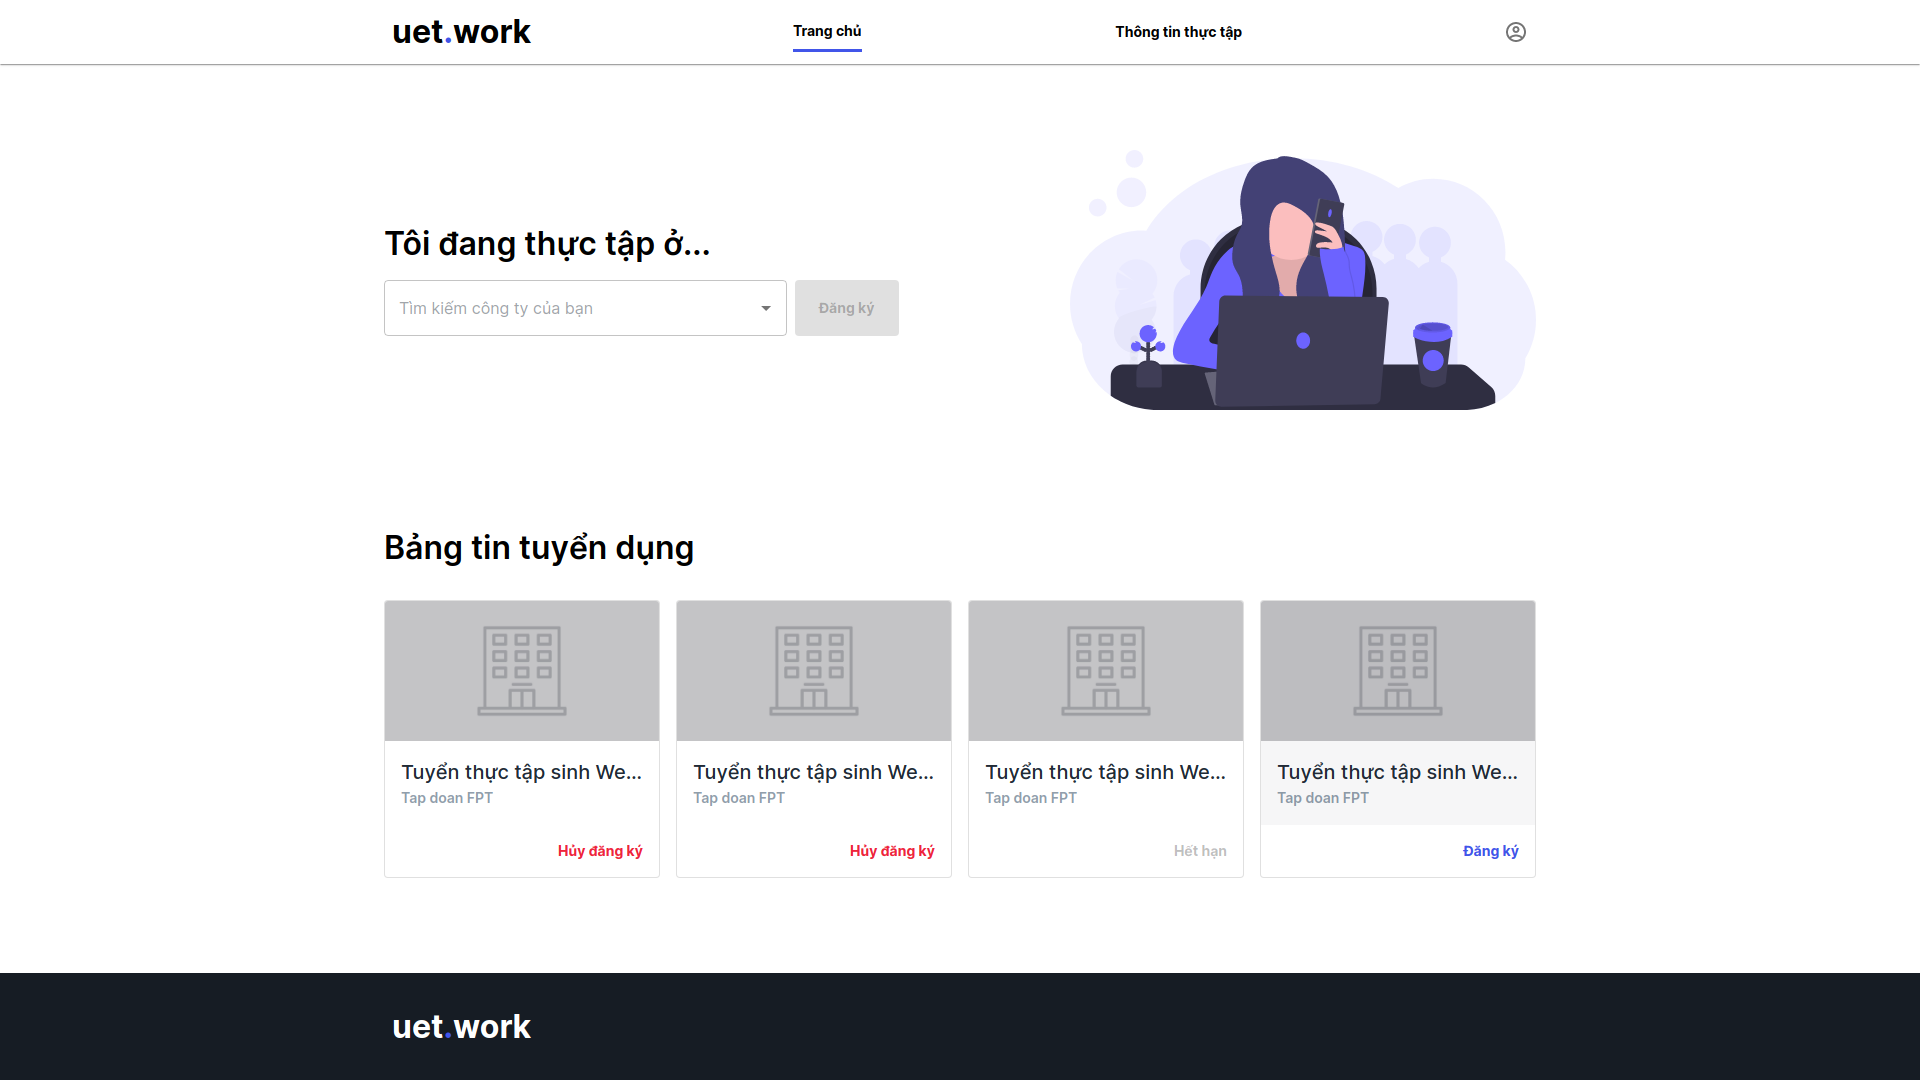
\includegraphics[width=\linewidth]{./images/image37.png}
	\caption{Luồng \emph{Đọc bài đăng}: Truy cập trang chủ và chọn bài đăng muốn đọc}
	\label{fig:student_home_page}
\end{figure}

\begin{figure}[]
	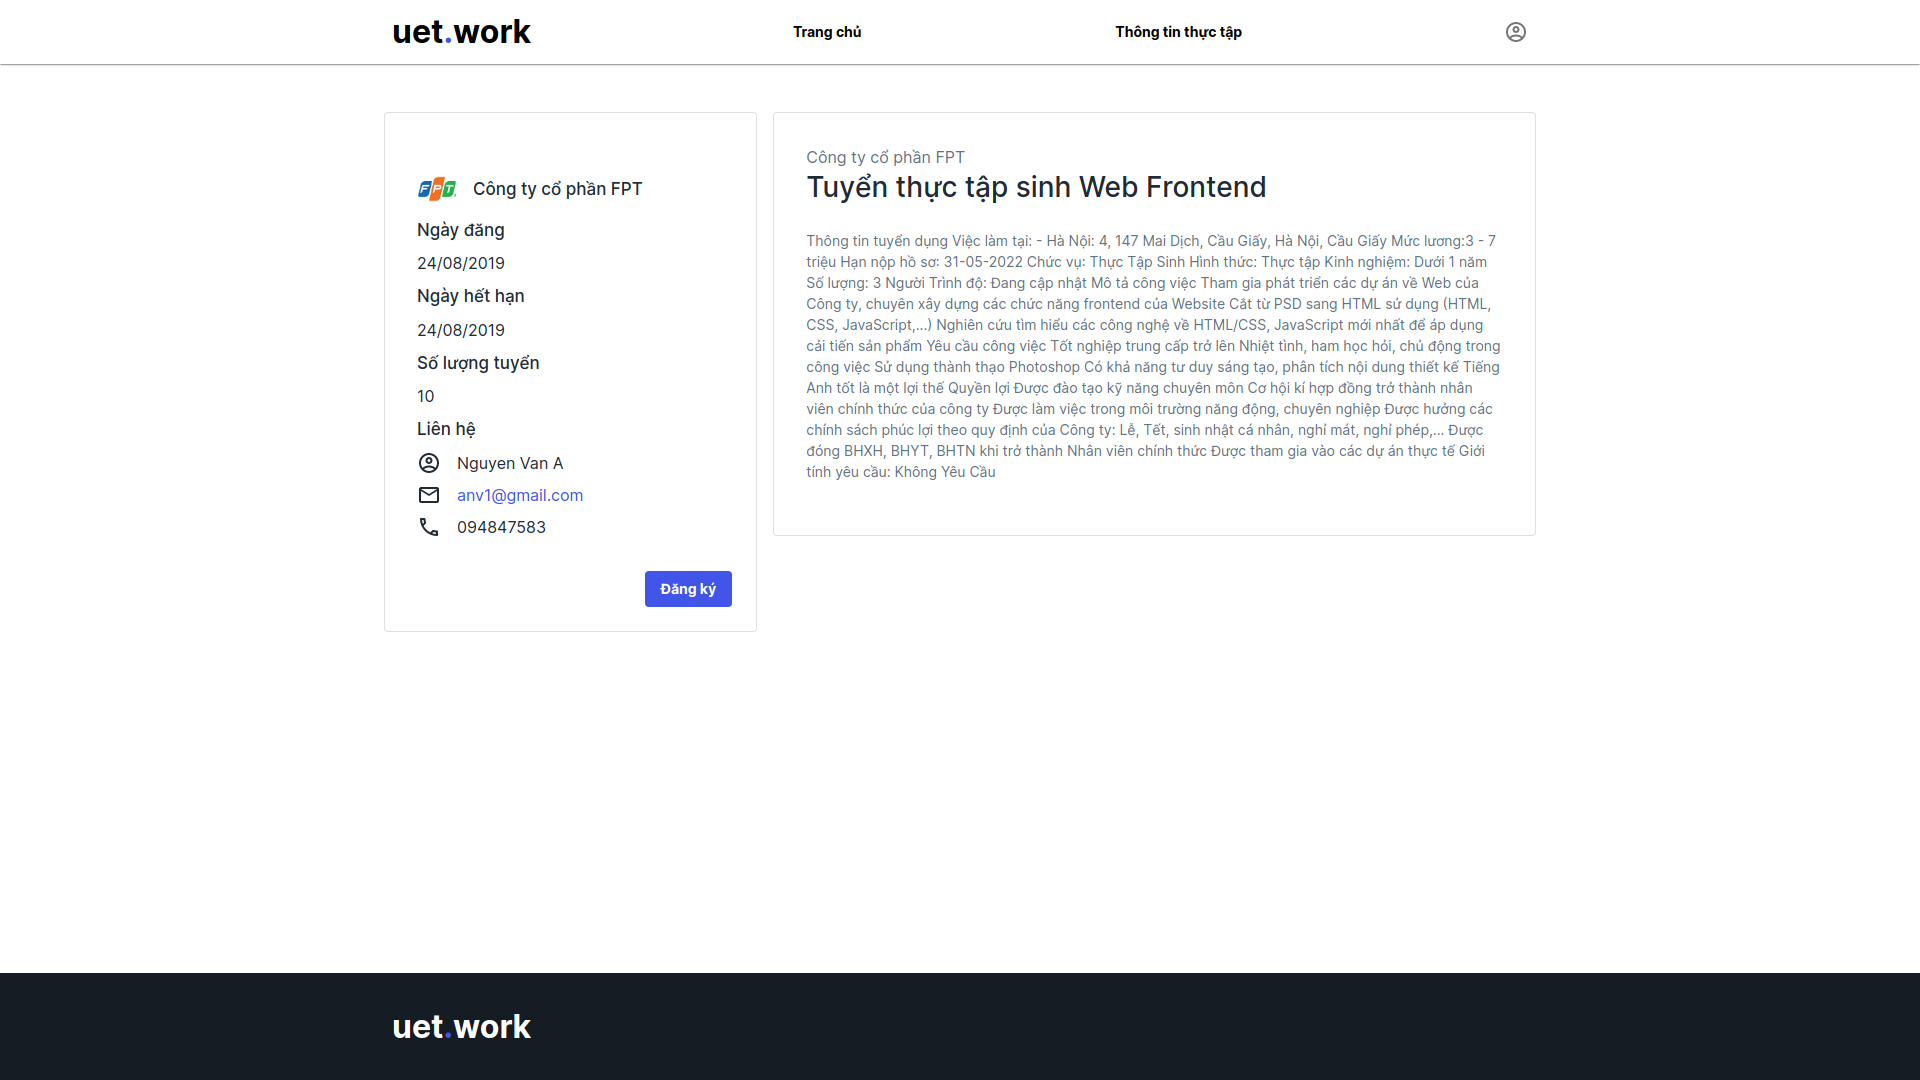
\includegraphics[width=\linewidth]{./images/image81.png}
	\caption{Luồng \emph{Đọc bài đăng}: Giao diện hiển thị bài đăng đã chọn}
	\label{fig:student_read_post_page}
\end{figure}

\paragraph*{Sinh viên đăng ký thực tập}

\begin{itemize}
	\item Hình \ref{fig:student_find_company}: Sinh viên tìm kiếm công ty mà mình đang thực tập và đăng ký. 
	\item Hình \ref{fig:student_register_company_success}: Nếu thành công, hệ thống hiển thị thông báo đăng ký thành công.
	\item Hình \ref{fig:student_register_company_failed}: Nếu thất bại, hệ thống hiển thị thông báo đăng ký thất bại.
\end{itemize}

\begin{figure}[]
	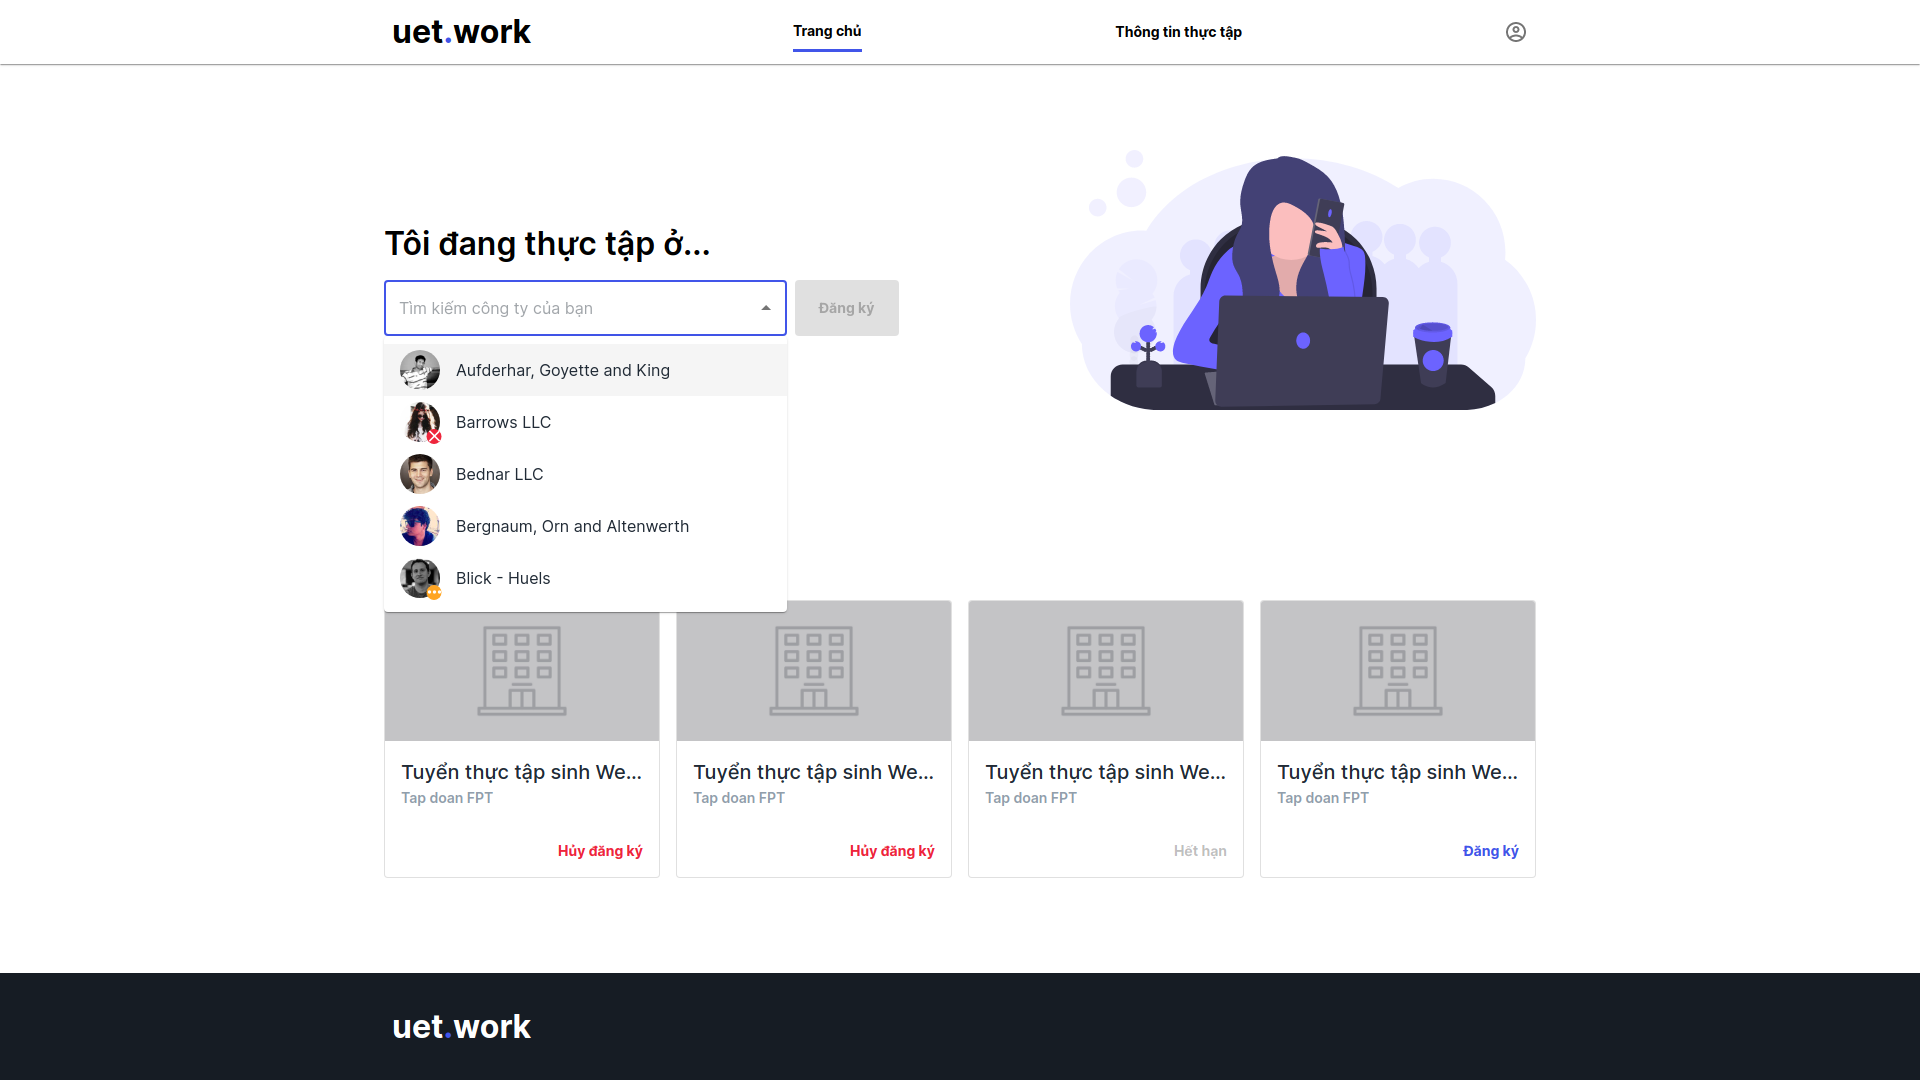
\includegraphics[width=\linewidth]{./images/image39.png}
	\caption{Luồng \emph{Sinh viên đăng ký thực tập}: Tìm kiếm công ty}
	\label{fig:student_find_company}
\end{figure}

\begin{figure}[]
	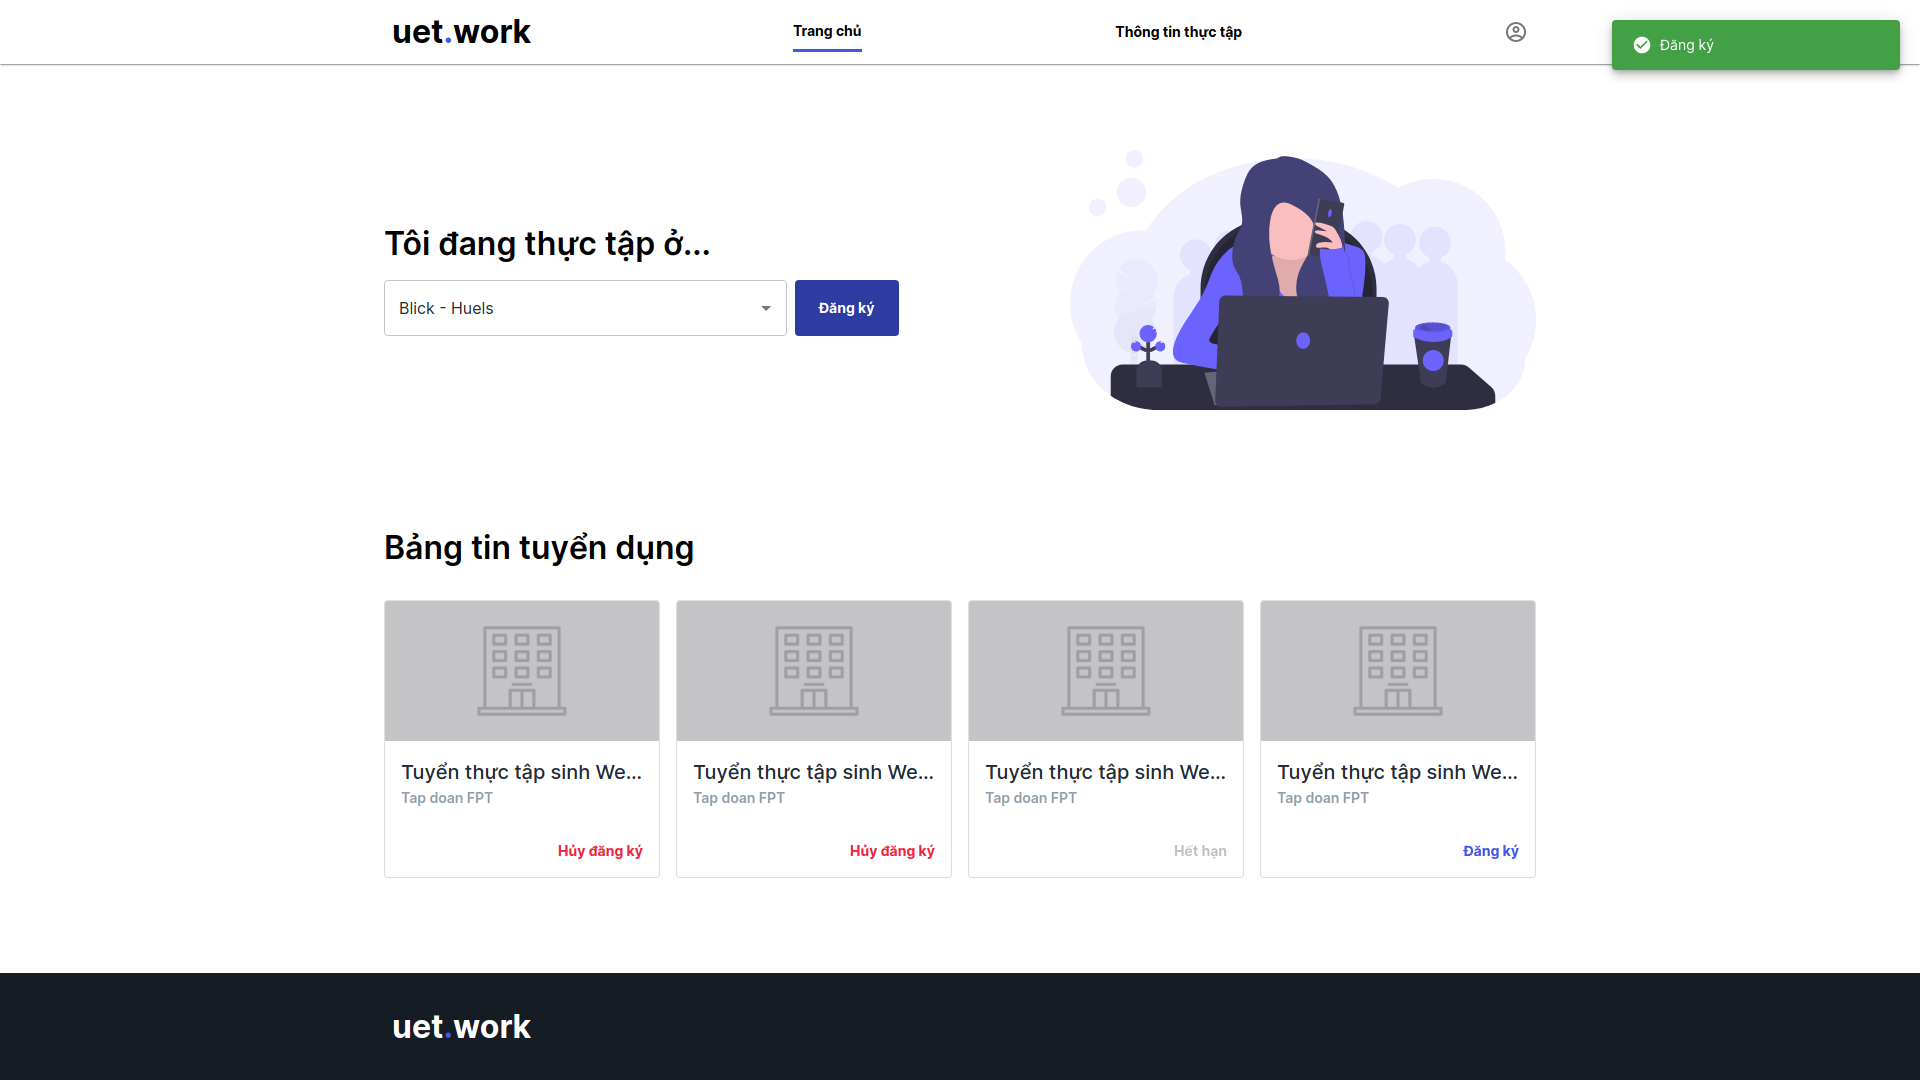
\includegraphics[width=\linewidth]{./images/image40-1.png}
	\caption{Luồng \emph{Sinh viên đăng ký thực tập}: Đăng ký thành công}
	\label{fig:student_register_company_success}
\end{figure}

\begin{figure}[]
	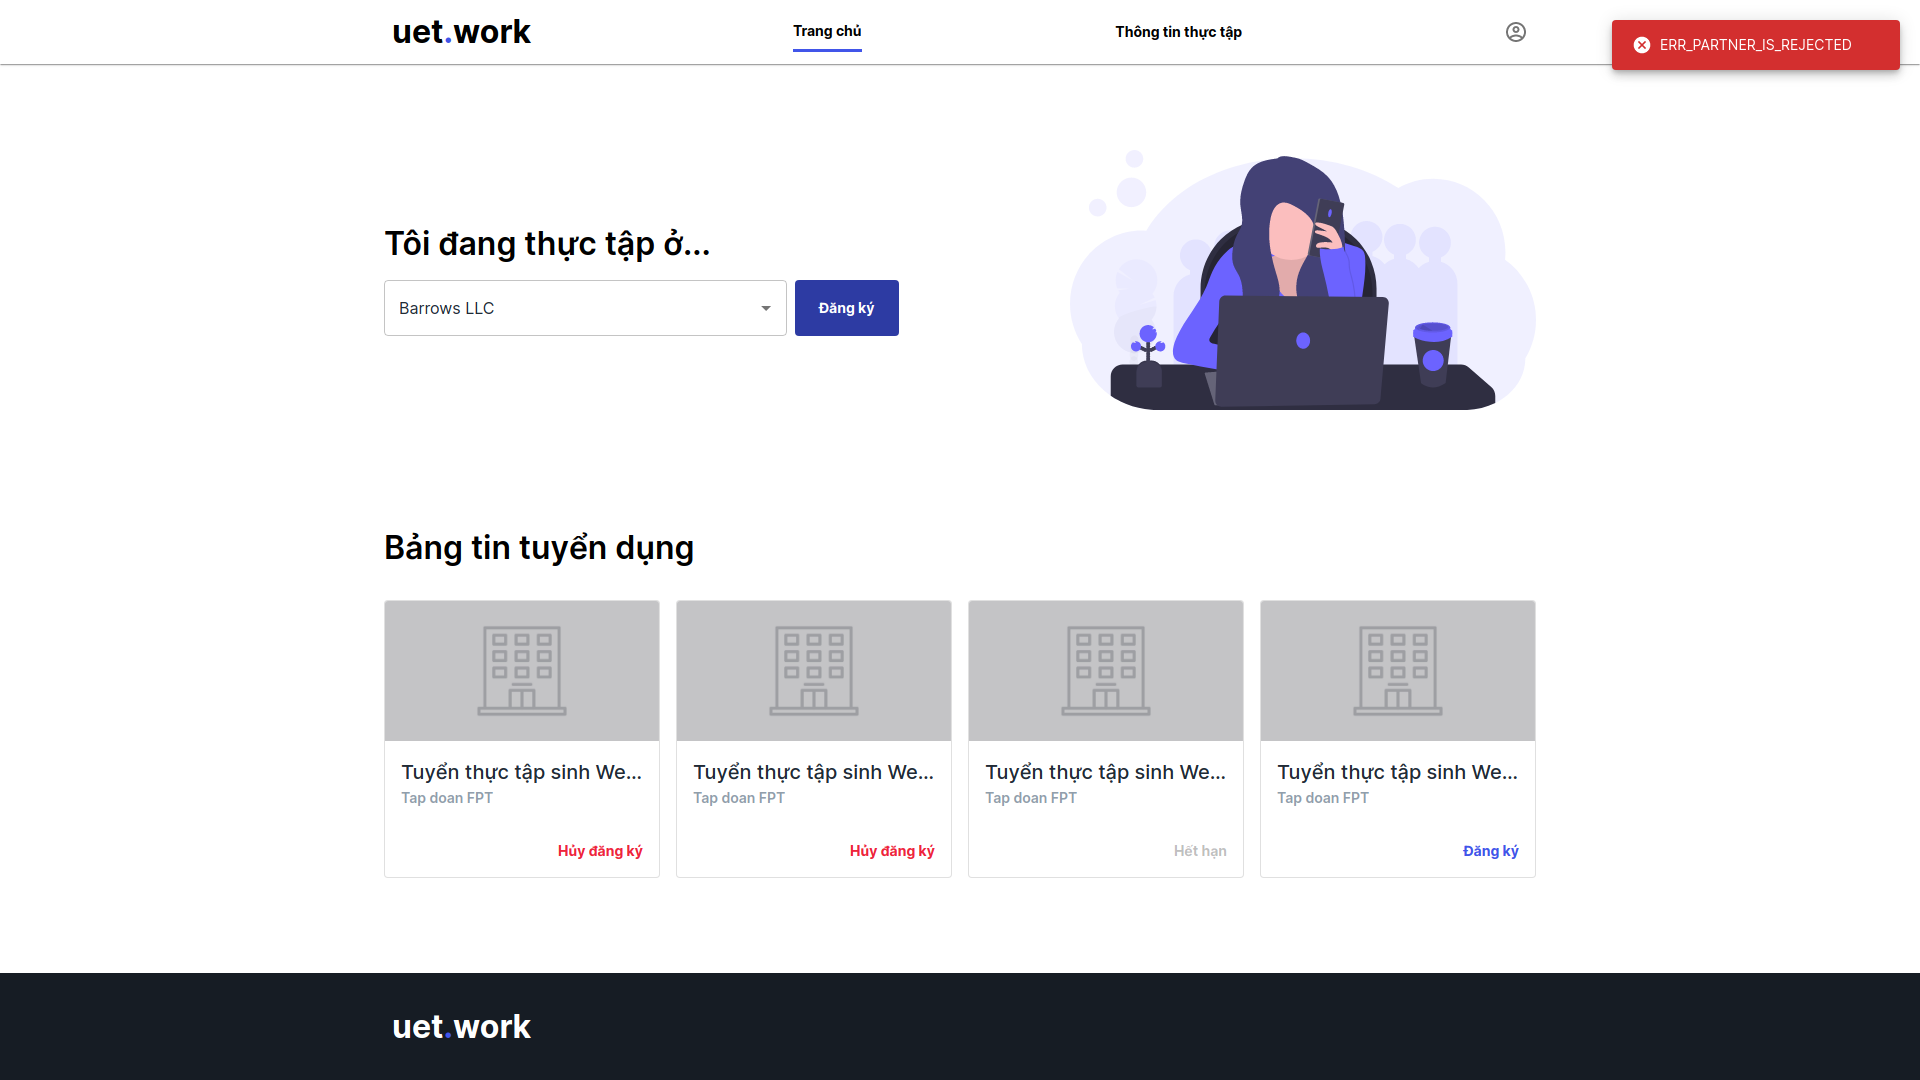
\includegraphics[width=\linewidth]{./images/image40.png}
	\caption{Luồng \emph{Sinh viên đăng ký thực tập}: Đăng ký thất bại}
	\label{fig:student_register_company_failed}
\end{figure}

\paragraph*{Sinh viên xem thông tin thực tập}
Sau khi đăng ký thực tập thành công, sinh viên vào kiểm tra thông tin thực tập của bản thân. Tại đây, sinh viên có thể xem thông tin công ty thực tập đã đúng chưa, giảng viên hướng dẫn là ai, và nộp báo cáo.

Hình \ref{fig:view_internship_page} mô tả màn hình trang thông tin thực tập.

\begin{figure}[]
	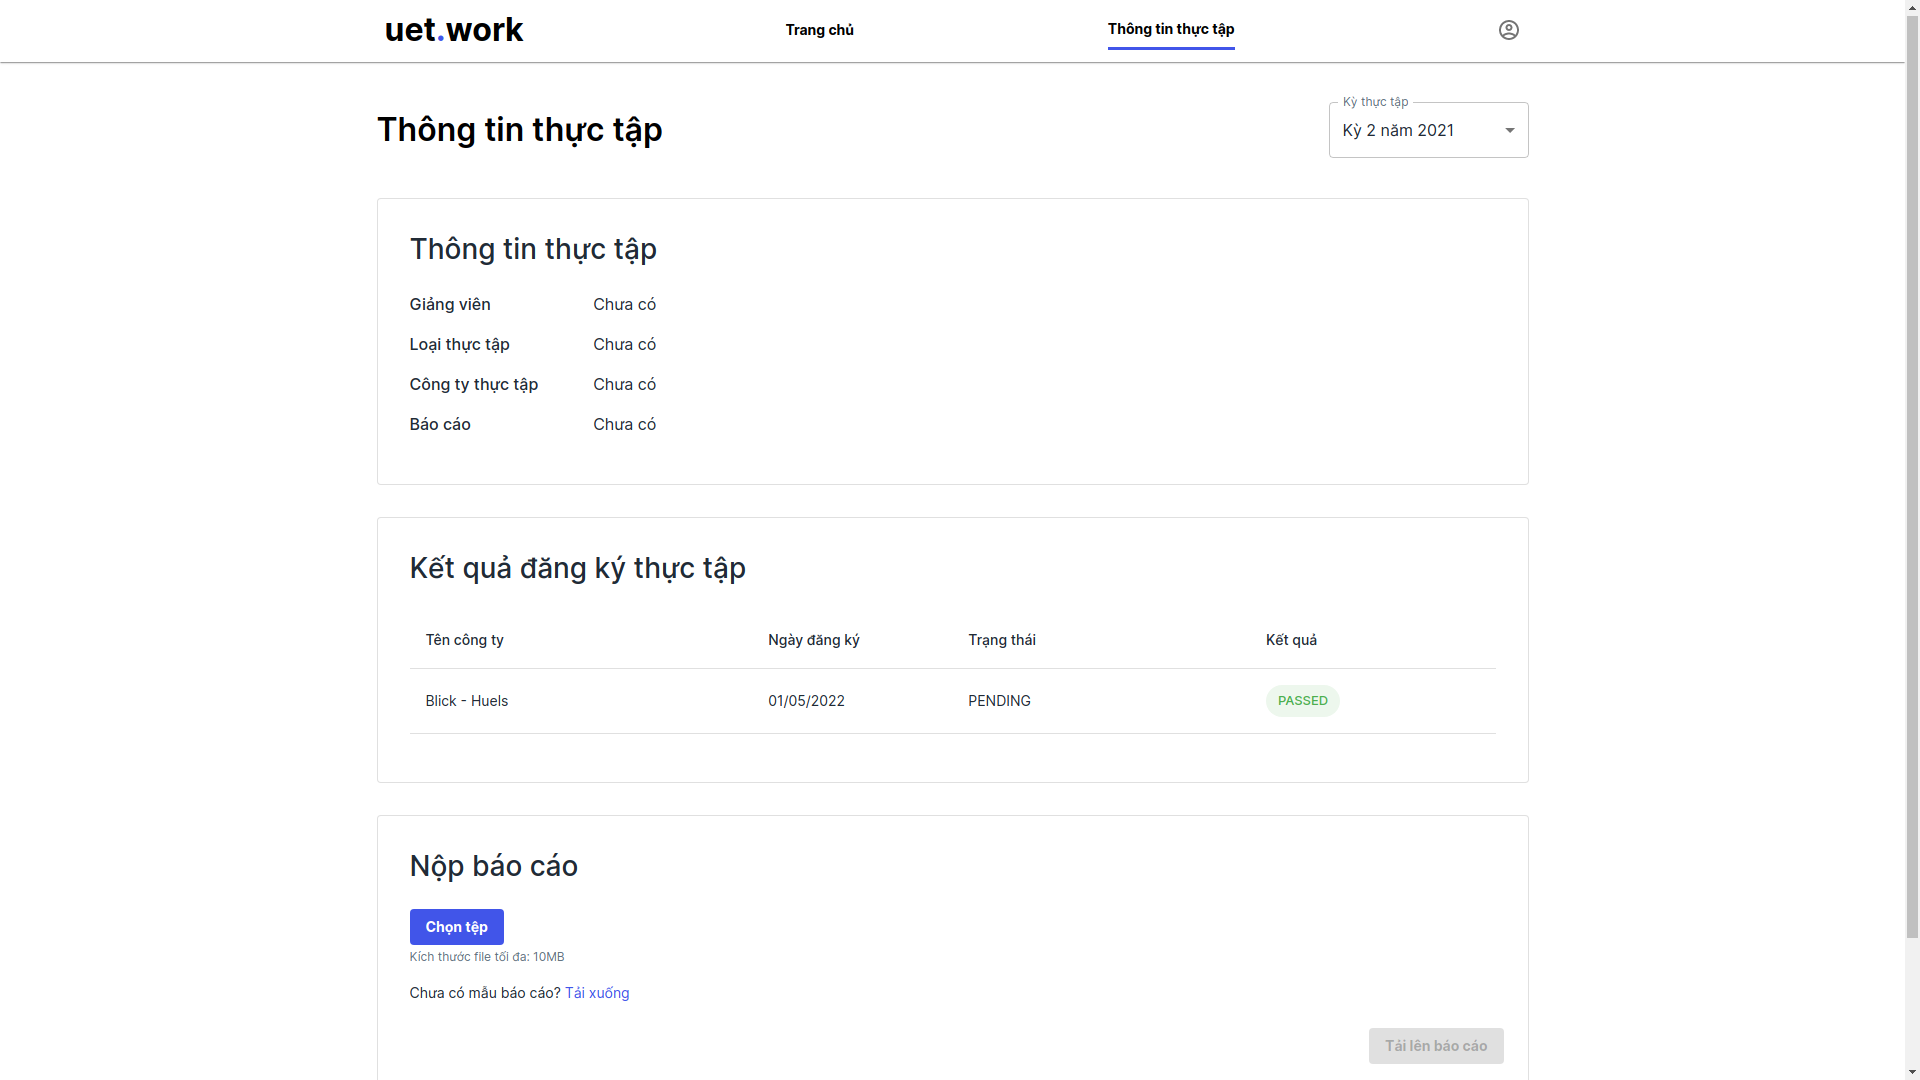
\includegraphics[width=\linewidth]{./images/image17.png}
	\caption{Luồng \emph{Sinh viên xem thông tin thực tập}}
	\label{fig:view_internship_page}
\end{figure}

\paragraph*{Sinh viên nộp báo cáo thực tập}

\begin{itemize}
	\item Hình \ref{fig:student_internship_info}: Sinh viên truy cập trang thông tin thực tập và kéo xuống phần Nộp báo cáo. 
	\item Hình \ref{fig:student_choose_file}: Sinh viên chọn tệp.
	\item Hình \ref{fig:student_upload_report}: Sinh viên tải lên báo cáo.
\end{itemize}

\begin{figure}[]
	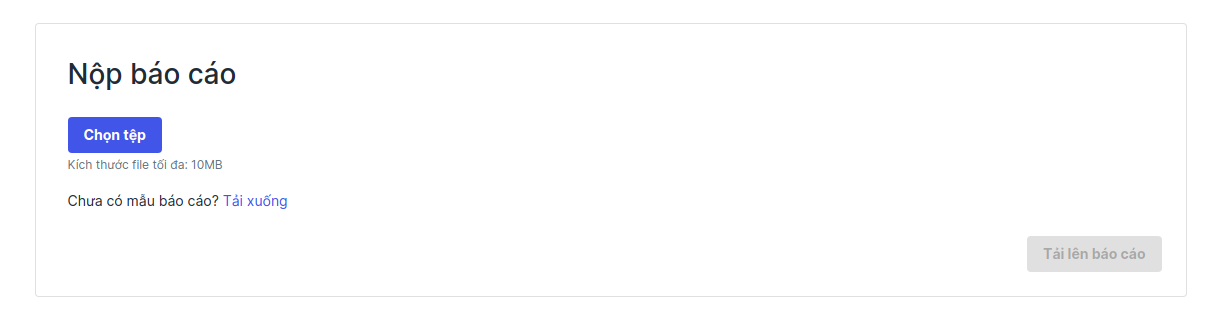
\includegraphics[width=\linewidth]{./images/image41.png}
	\caption{Luồng \emph{Sinh viên nộp báo cáo}: Truy cập phần nộp báo cáo}
	\label{fig:student_internship_info}
\end{figure}

\begin{figure}[]
	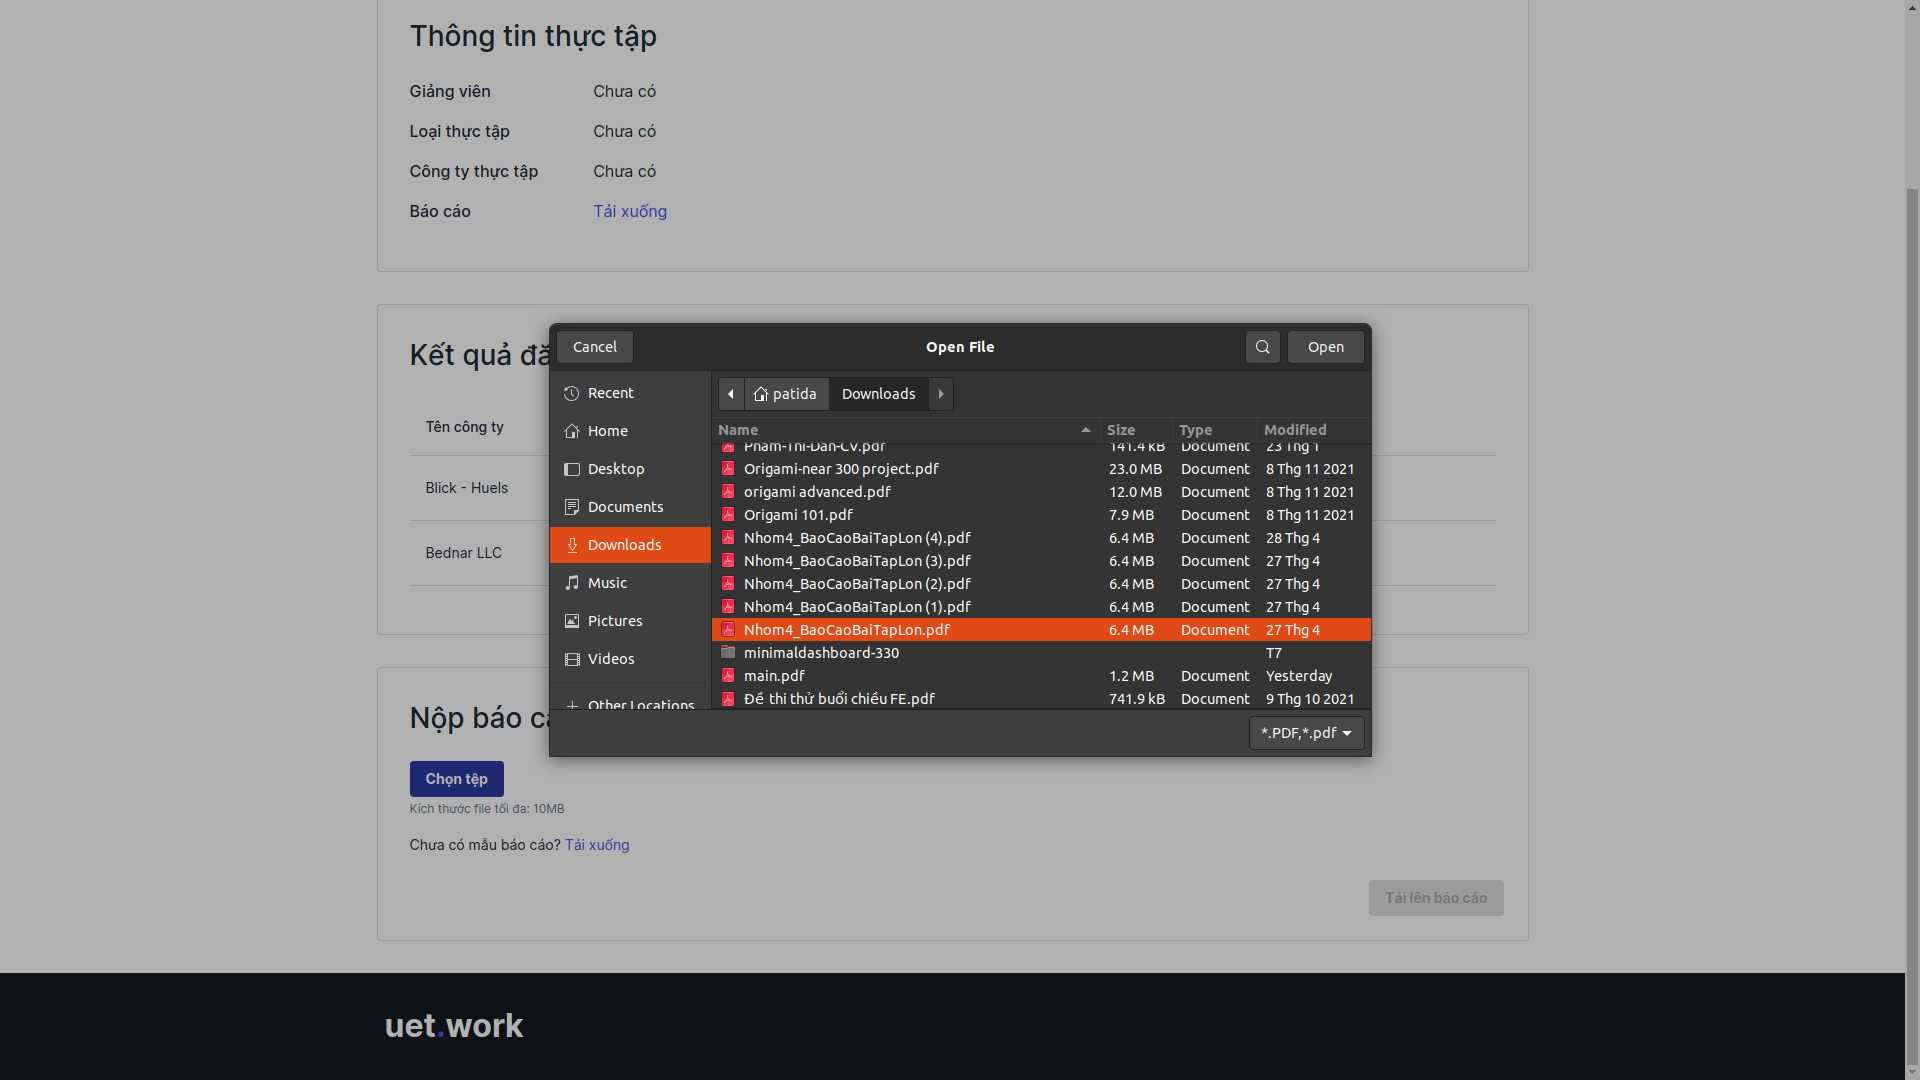
\includegraphics[width=\linewidth]{./images/image42.png}
	\caption{Luồng \emph{Sinh viên nộp báo cáo}: Chọn tệp}
	\label{fig:student_choose_file}
\end{figure}

\begin{figure}[]
	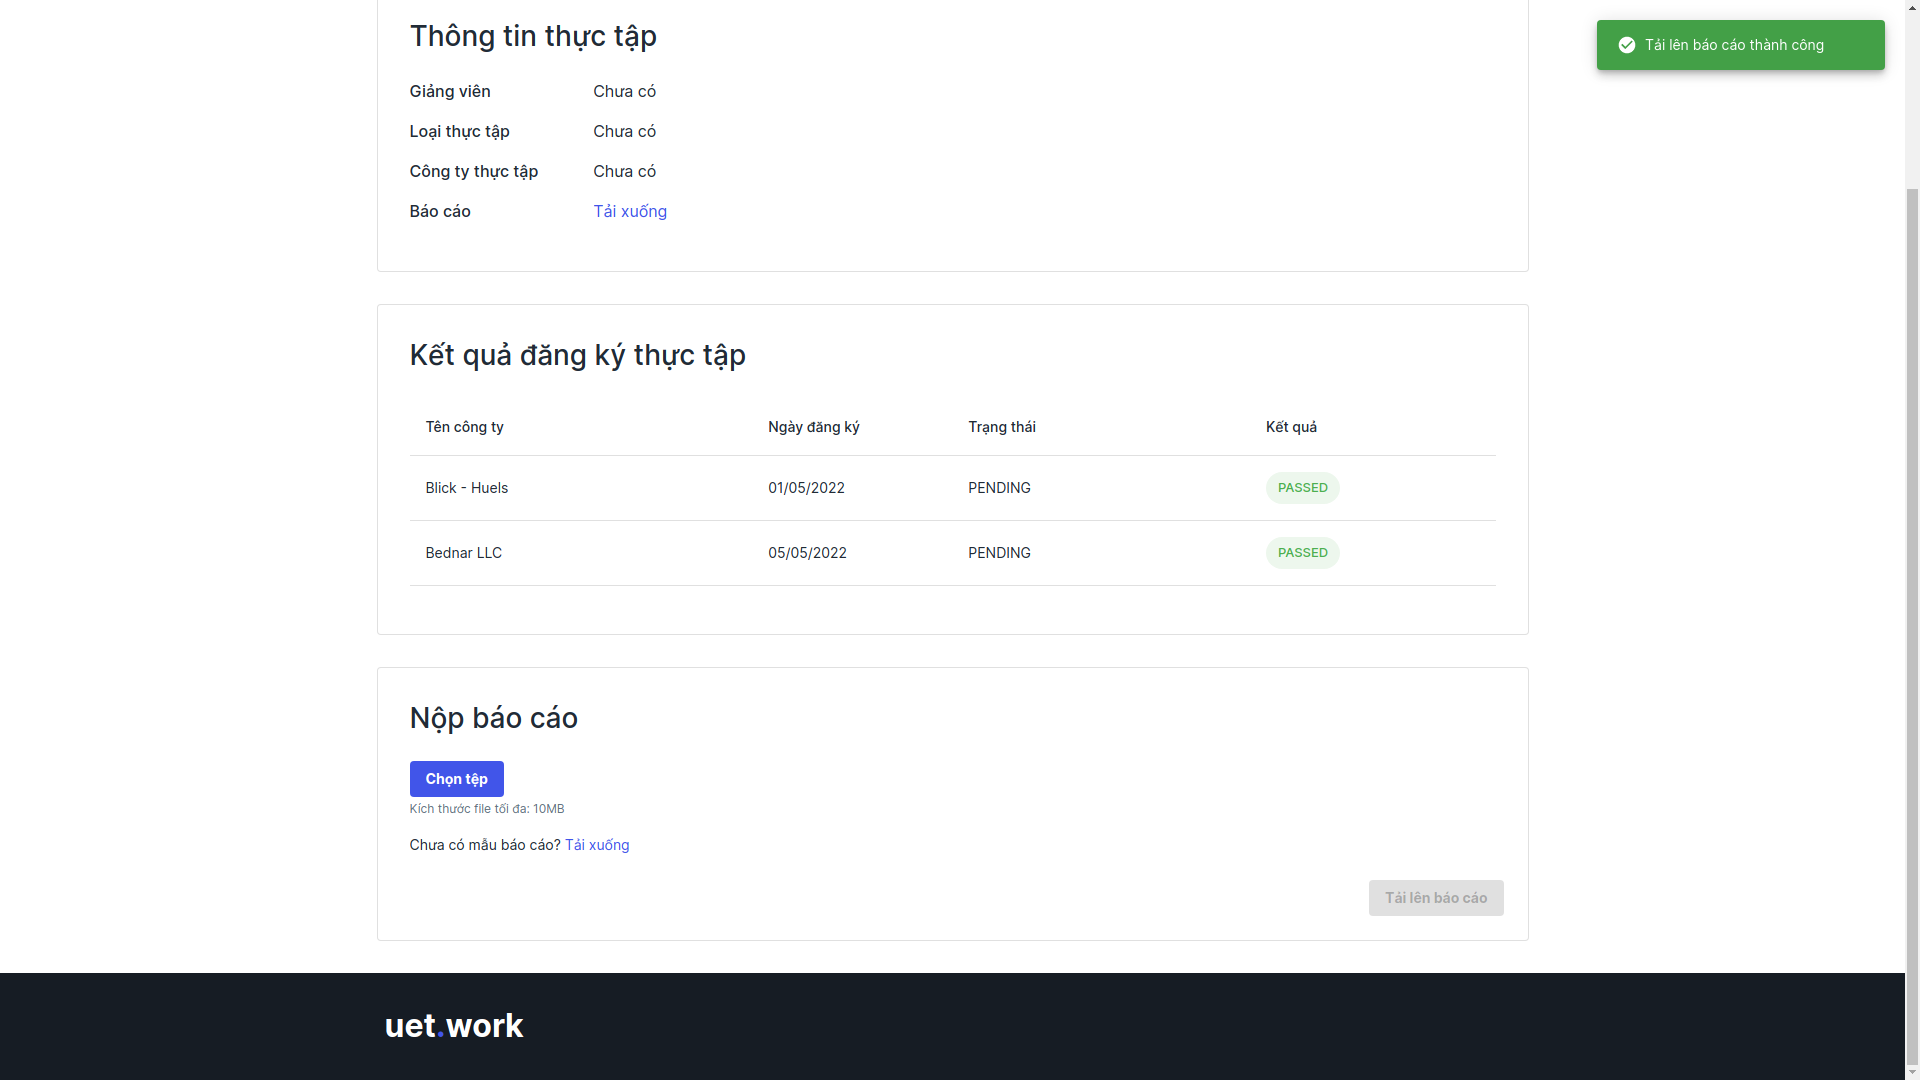
\includegraphics[width=\linewidth]{./images/image43.png}
	\caption{Luồng \emph{Sinh viên nộp báo cáo}: Tải lên báo cáo}
	\label{fig:student_upload_report}
\end{figure}

\paragraph*{Sinh viên xem thông tin cá nhân}
Sinh viên truy cập trang thông tin cá nhân. Tại đây sinh viên có thể sửa thông tin cá nhân, đổi mật khẩu.

Hình \ref{fig:view_info_page} mô tả màn hình trang thông tin cá nhân.

\begin{figure}[]
	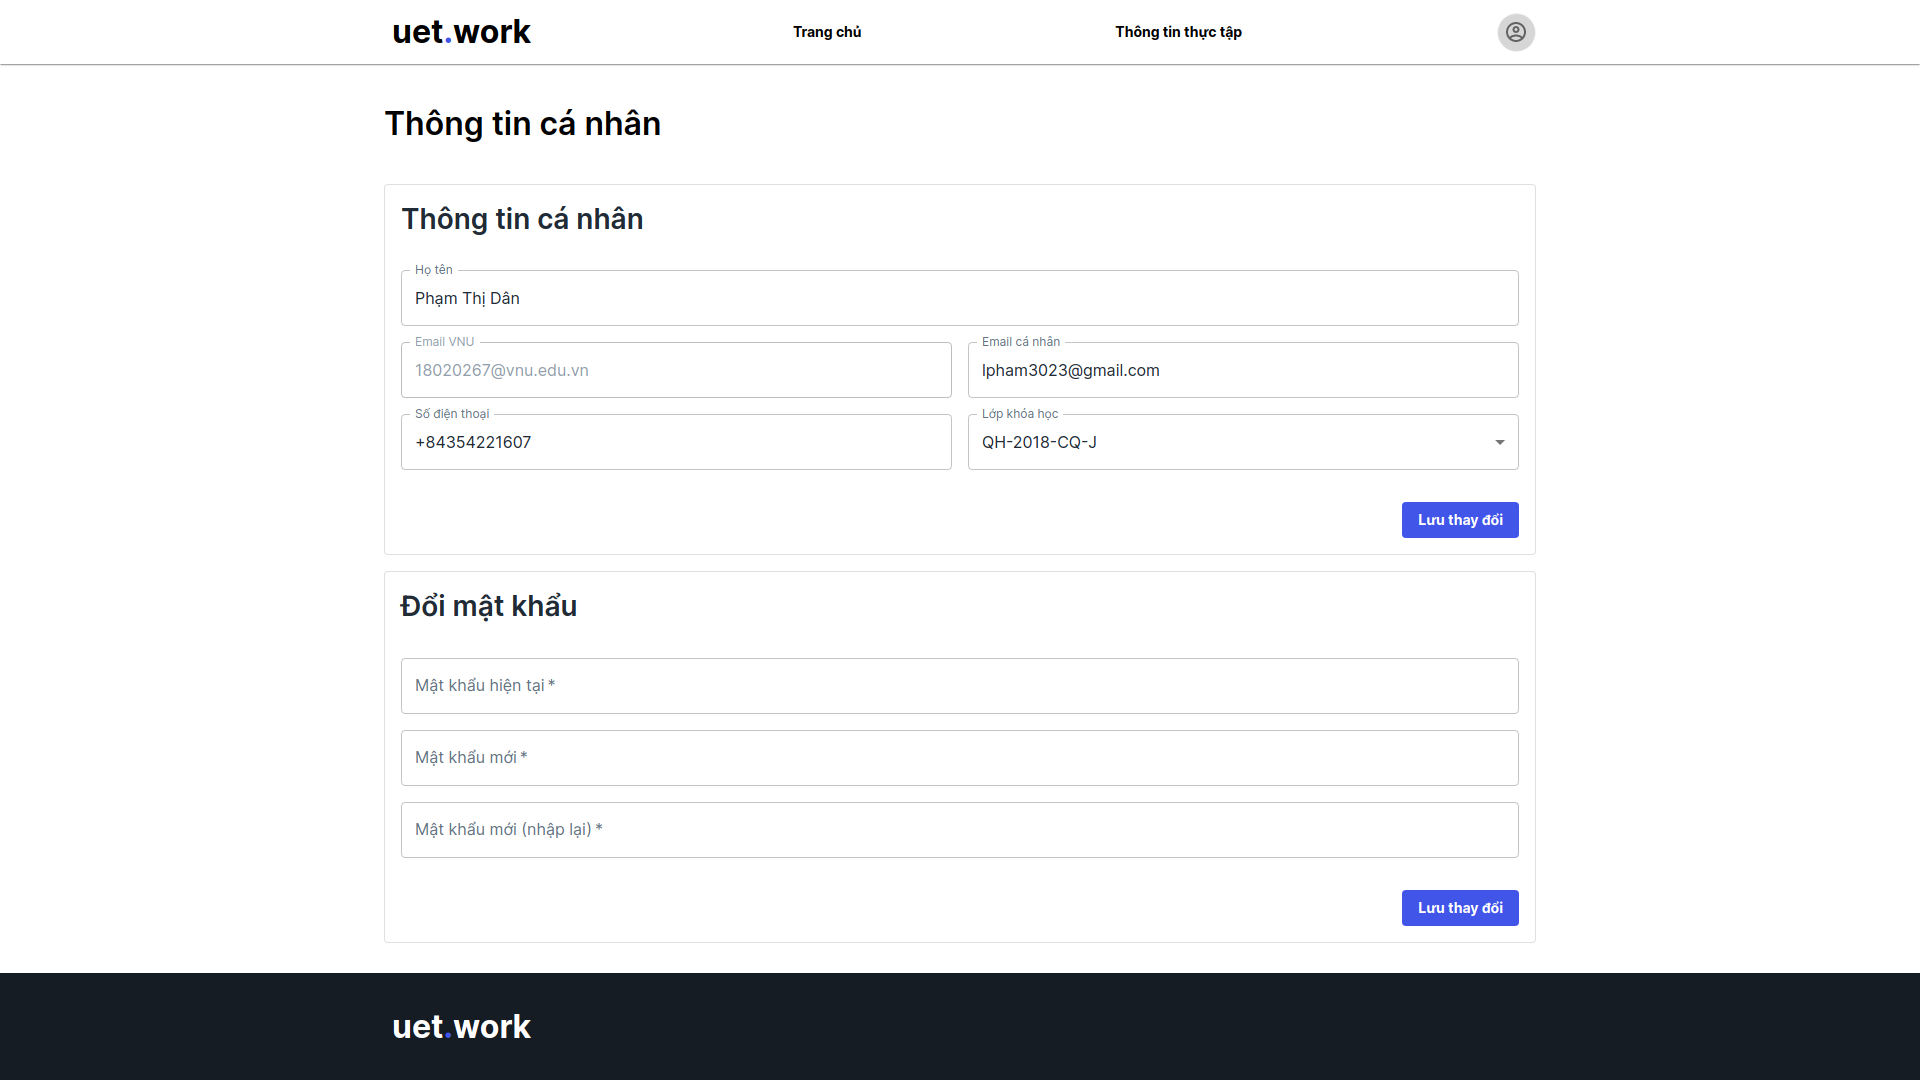
\includegraphics[width=\linewidth]{./images/image44.png}
	\caption{Luồng \emph{Sinh viên xem thông tin cá nhân}}
	\label{fig:view_info_page}
\end{figure}

\paragraph*{Sinh viên thay đổi thông tin cá nhân}

\begin{itemize}
	\item Hình \ref{fig:student_access_info}: Sinh viên truy cập phần thông tin cá nhân. 
	\item Hình \ref{fig:student_edit_info}: Sinh viên sửa thông tin cá nhân, đổi mật khẩu.
\end{itemize}

\begin{figure}[]
	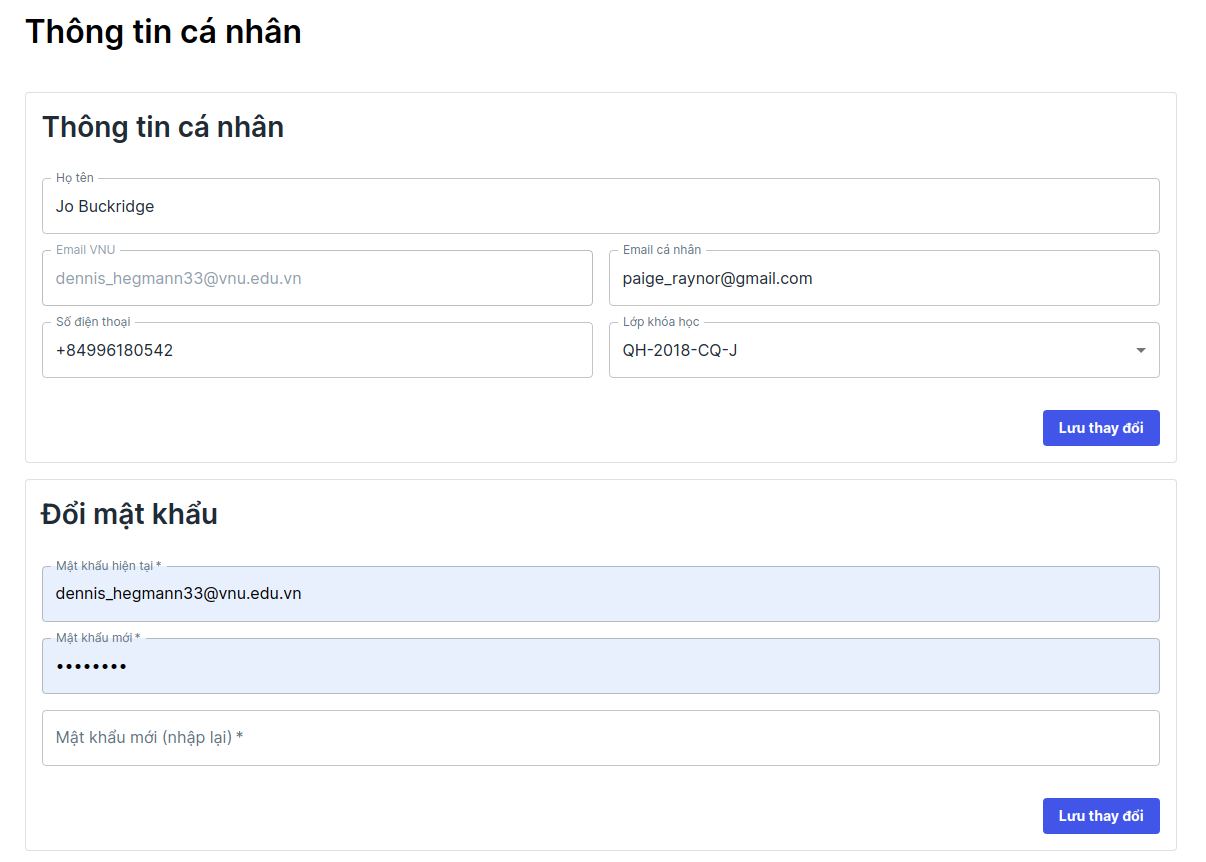
\includegraphics[width=\linewidth]{./images/image45.png}
	\caption{Luồng \emph{Sinh viên thay đổi thông tin cá nhân}: Truy cập trang thông tin cá nhân}
	\label{fig:student_access_info}
\end{figure}

\begin{figure}[]
	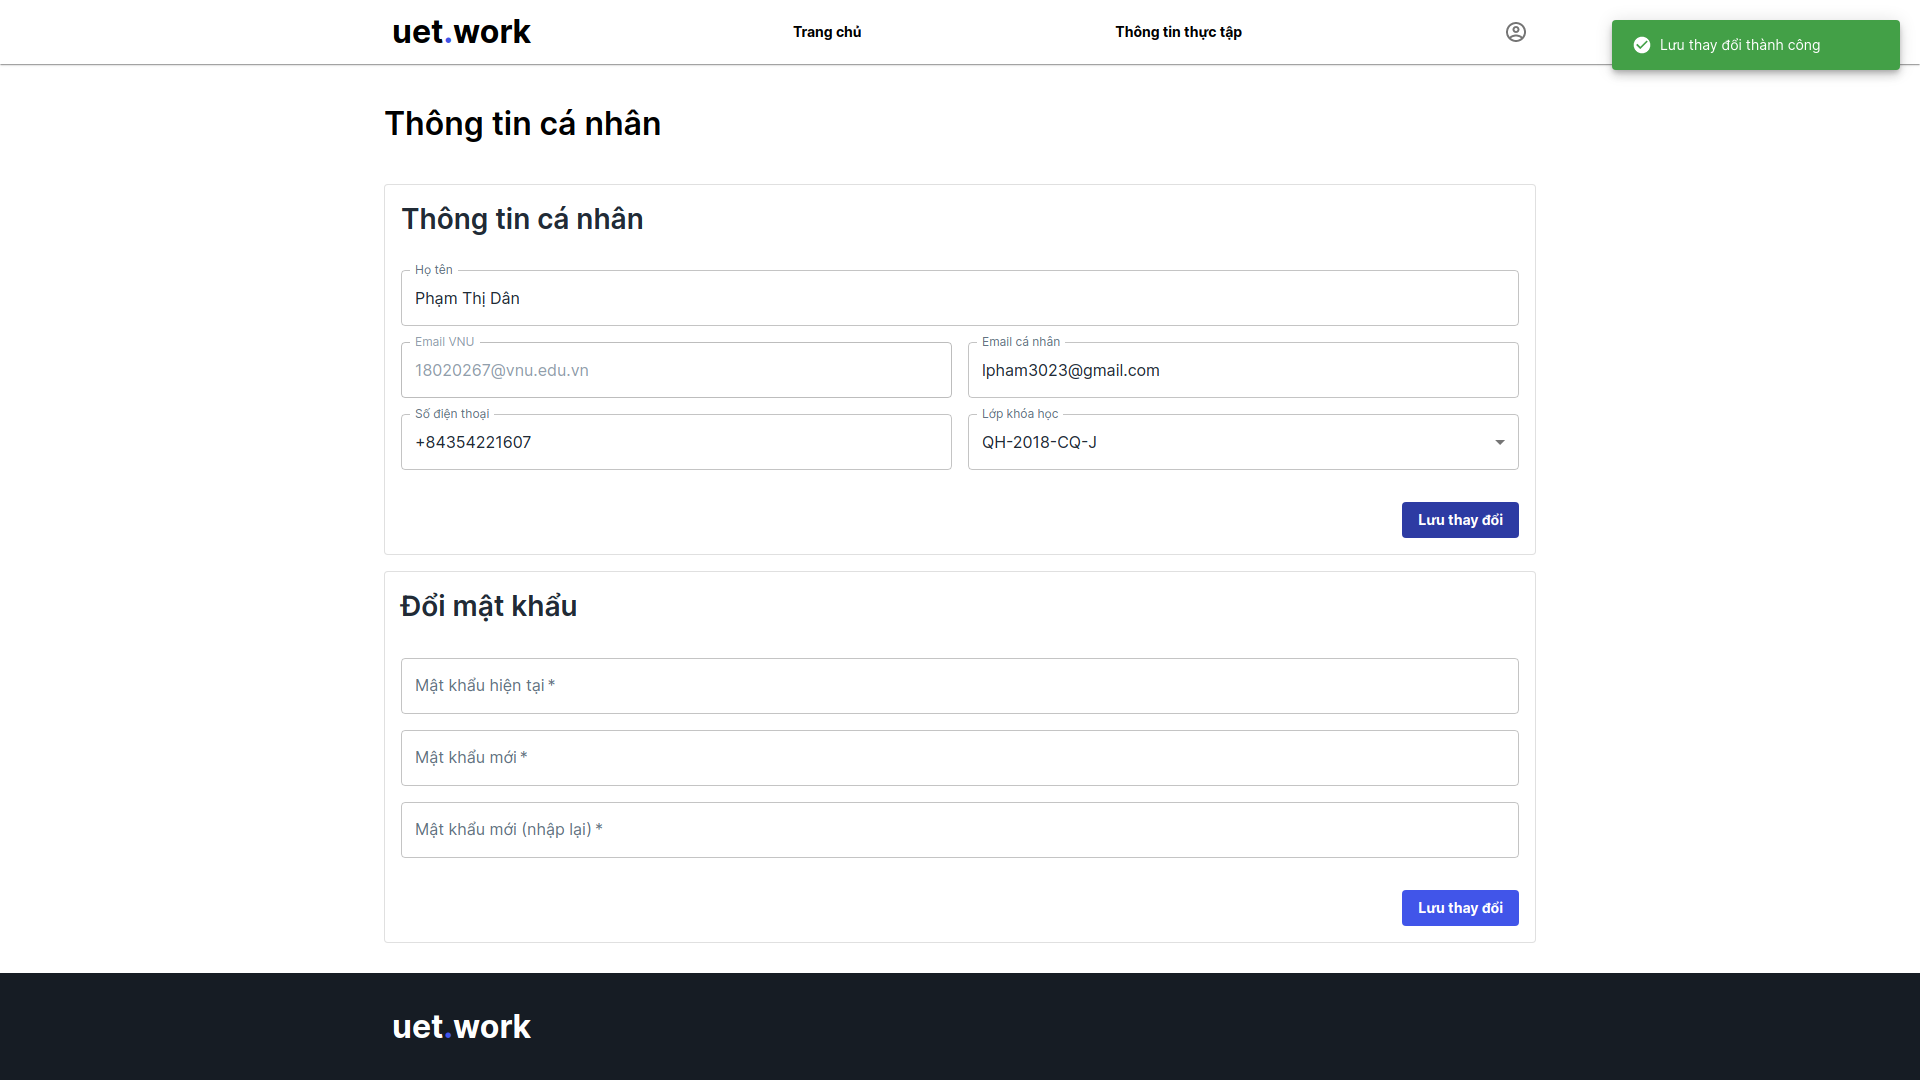
\includegraphics[width=\linewidth]{./images/image46.png}
	\caption{Luồng \emph{Sinh viên thay đổi thông tin cá nhân}: Sinh viên thay đổi thông tin cá nhân}
	\label{fig:student_edit_info}
\end{figure}

\subsection{Luồng sử dụng của giảng viên}

\paragraph*{Giảng viên xem danh sách sinh viên đang hướng dẫn}

Giảng viên truy cập trang Sinh viên đang hướng dẫn. Tại đây, giảng viên có thể tìm kiếm, sắp xếp, lọc danh sách theo kỳ thực tập, trạng thái báo cáo, trạng thái chấm điểm.

Hình \ref{fig:working_student_page} mô tả màn hình danh sách sinh viên đang hướng dẫn.

\begin{figure}[]
	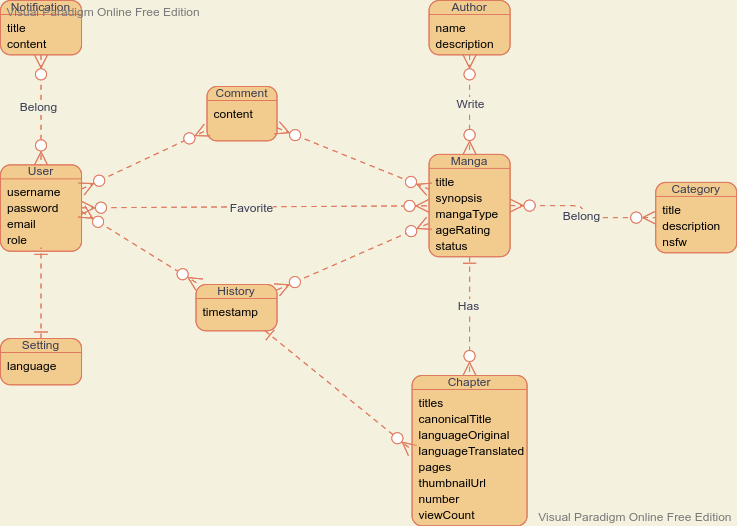
\includegraphics[width=\linewidth]{./images/image8.png}
	\caption{Luồng \emph{Giảng viên xem danh sách sinh viên đang hướng dẫn}}
	\label{fig:working_student_page}
\end{figure}

\paragraph*{Giảng viên tải xuống báo cáo}
Hình \ref{fig:lecturer_access_students}: Giảng viên truy cập trang sinh viên đang hướng dẫn và tải xuống báo cáo của sinh viên. 

\begin{figure}[]
	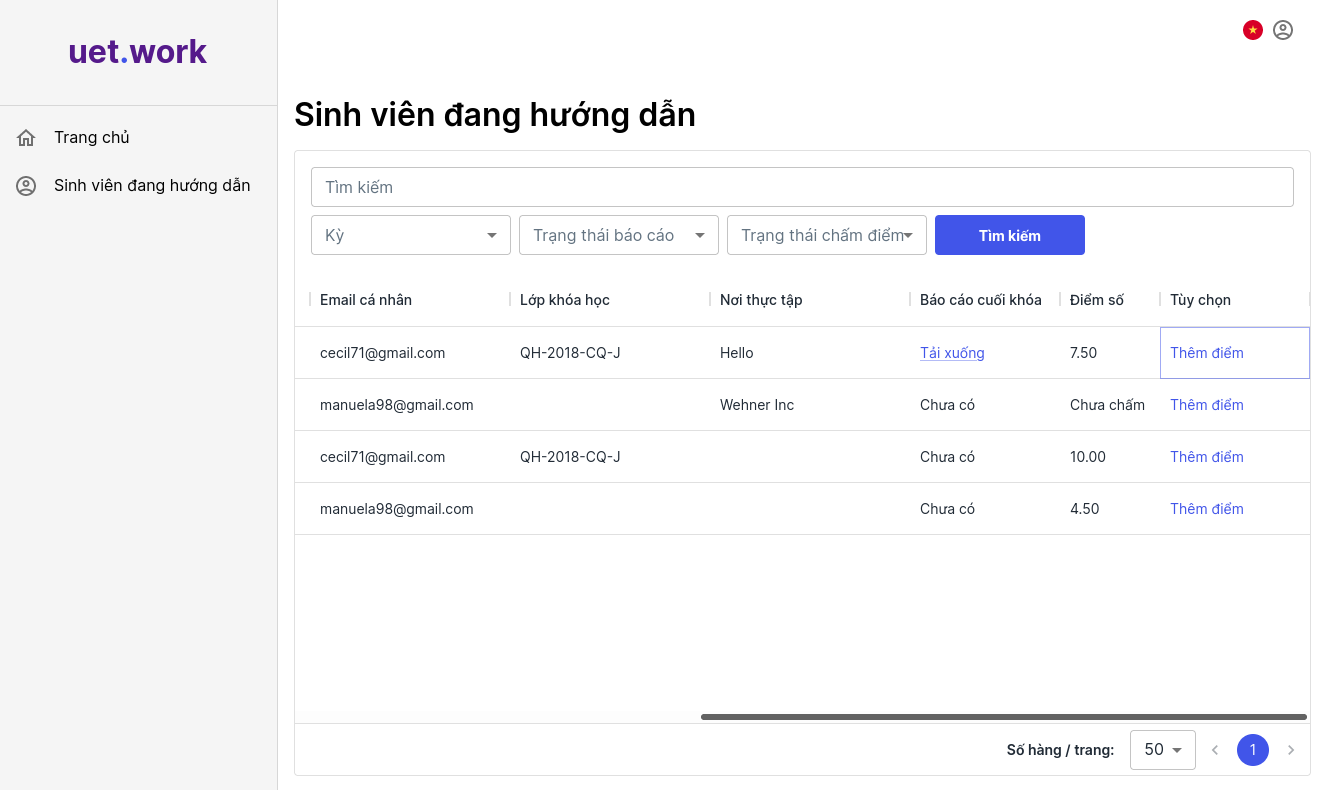
\includegraphics[width=\linewidth]{./images/image64.png}
	\caption{Luồng \emph{Giảng viên tải xuống báo cáo}}
	\label{fig:lecturer_access_students}
\end{figure}

\paragraph*{Giảng viên chấm điểm cho sinh viên}

\begin{itemize}
	\item Hình \ref{fig:lecturer_access_students_page}: Giảng viên truy cập trang sinh viên đang hướng dẫn. 
	\item Hình \ref{fig:lecturer_score}: Giảng viên chấm điểm cho sinh viên.
\end{itemize}

\begin{figure}[]
	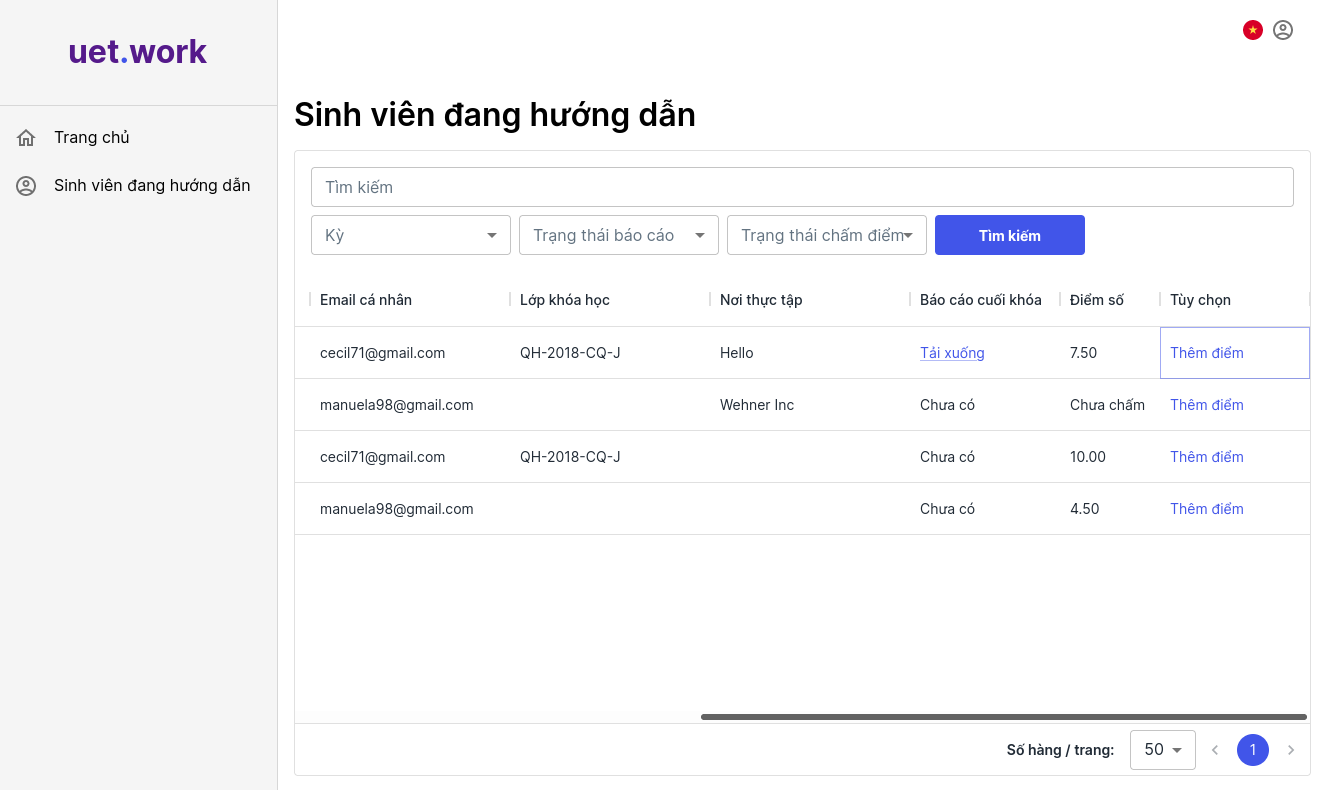
\includegraphics[width=\linewidth]{./images/image64.png}
	\caption{Luồng \emph{Giảng viên chấm điểm cho sinh viên}: Giảng viên truy cập trang sinh viên đang hướng dẫn}
	\label{fig:lecturer_access_students_page}
\end{figure}

\begin{figure}[]
	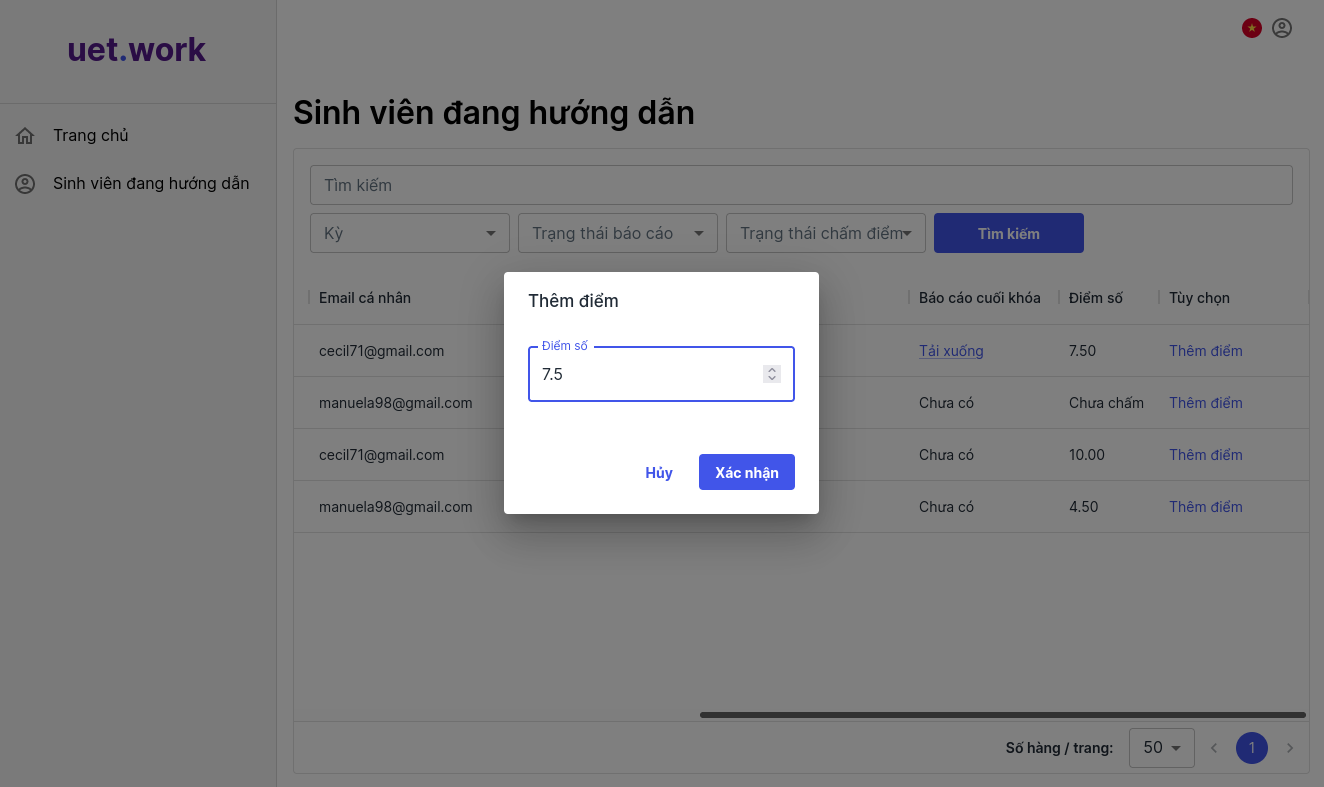
\includegraphics[width=\linewidth]{./images/image65.png}
	\caption{Luồng \emph{Giảng viên chấm điểm cho sinh viên}: Giảng viên chấm điểm cho sinh viên}
	\label{fig:lecturer_score}
\end{figure}

\paragraph*{Giảng viên thay đổi thông tin cá nhân}

\begin{itemize}
	\item Hình \ref{fig:lecturer_access_info_page}: Giảng viên truy cập trang thông tin cá nhân. 
	\item Hình \ref{fig:lecturer_edit_info}: Giảng viên thay đổi thông tin cá nhân.
\end{itemize}

\begin{figure}[]
	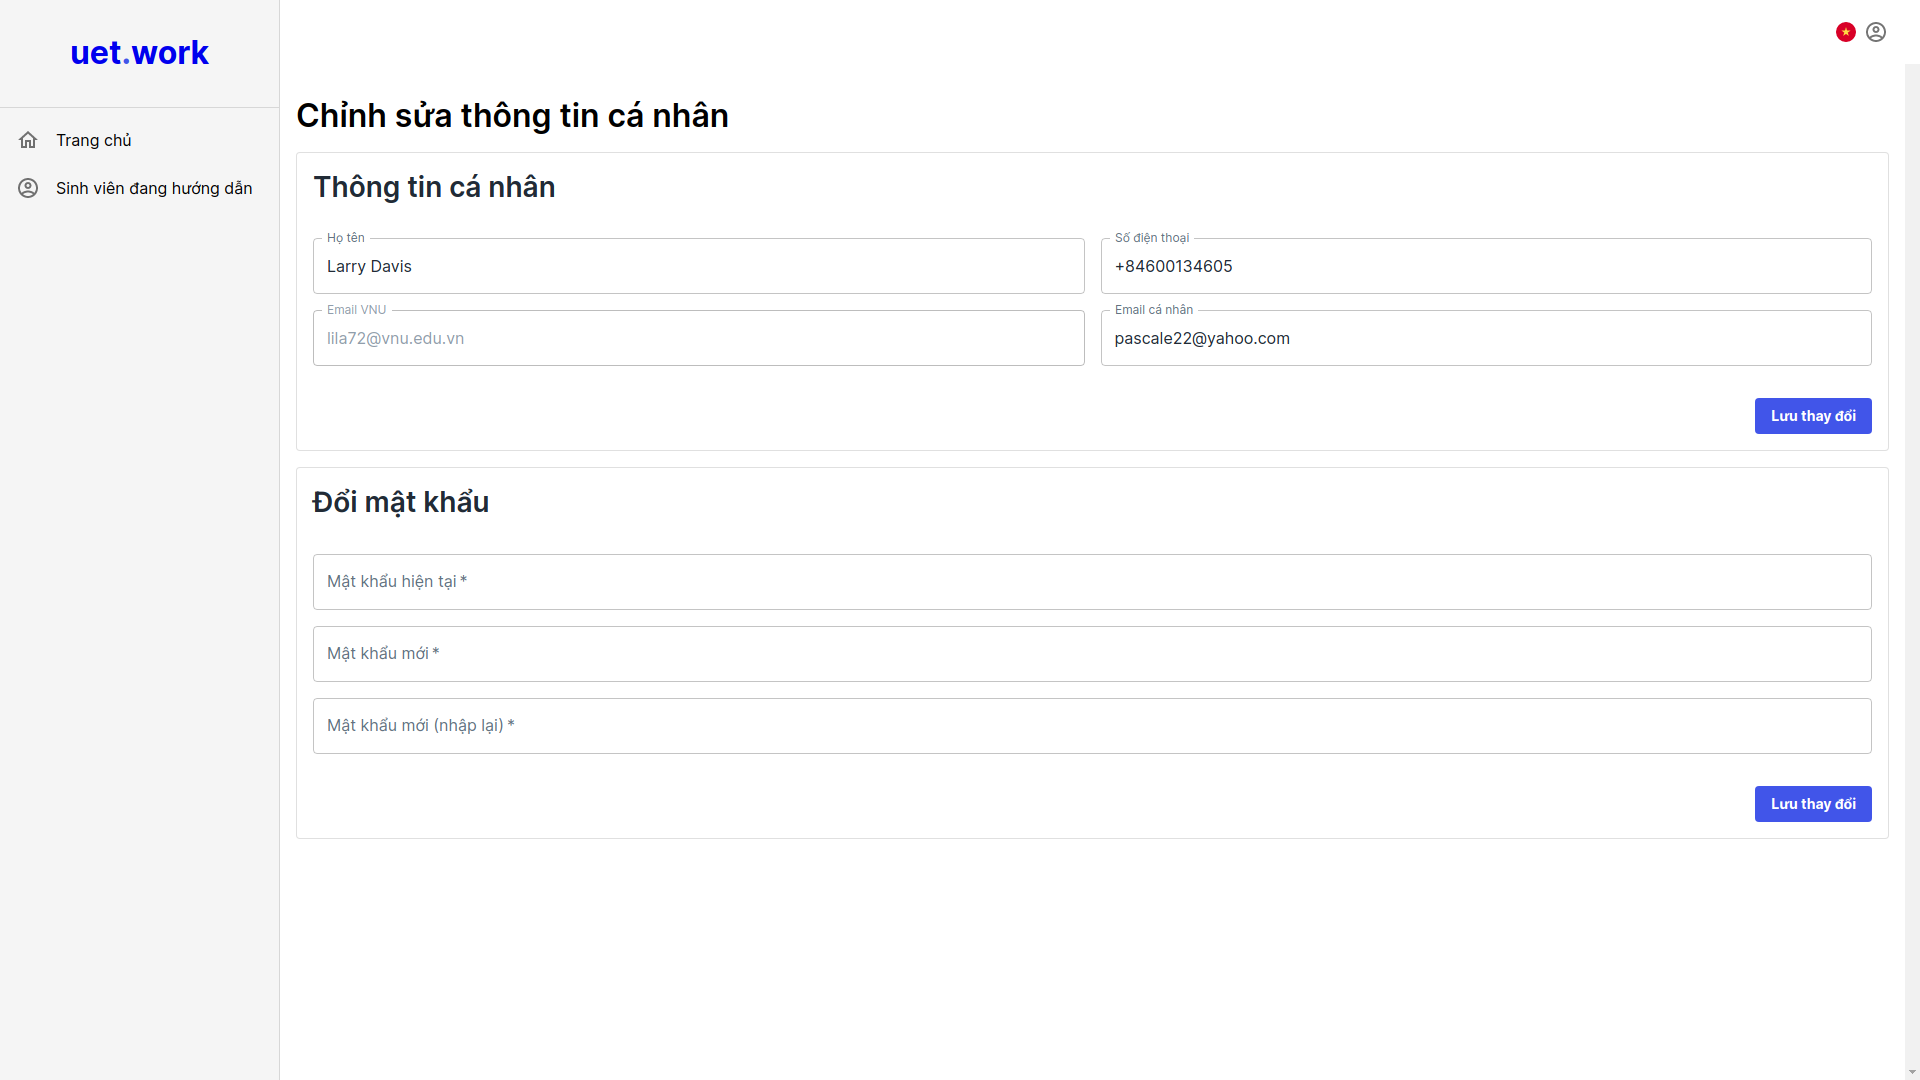
\includegraphics[width=\linewidth]{./images/image51.png}
	\caption{Luồng \emph{Giảng viên thay đổi thông tin cá nhân}: Giảng viên truy cập trang thông tin cá nhân}
	\label{fig:lecturer_access_info_page}
\end{figure}

\begin{figure}[]
	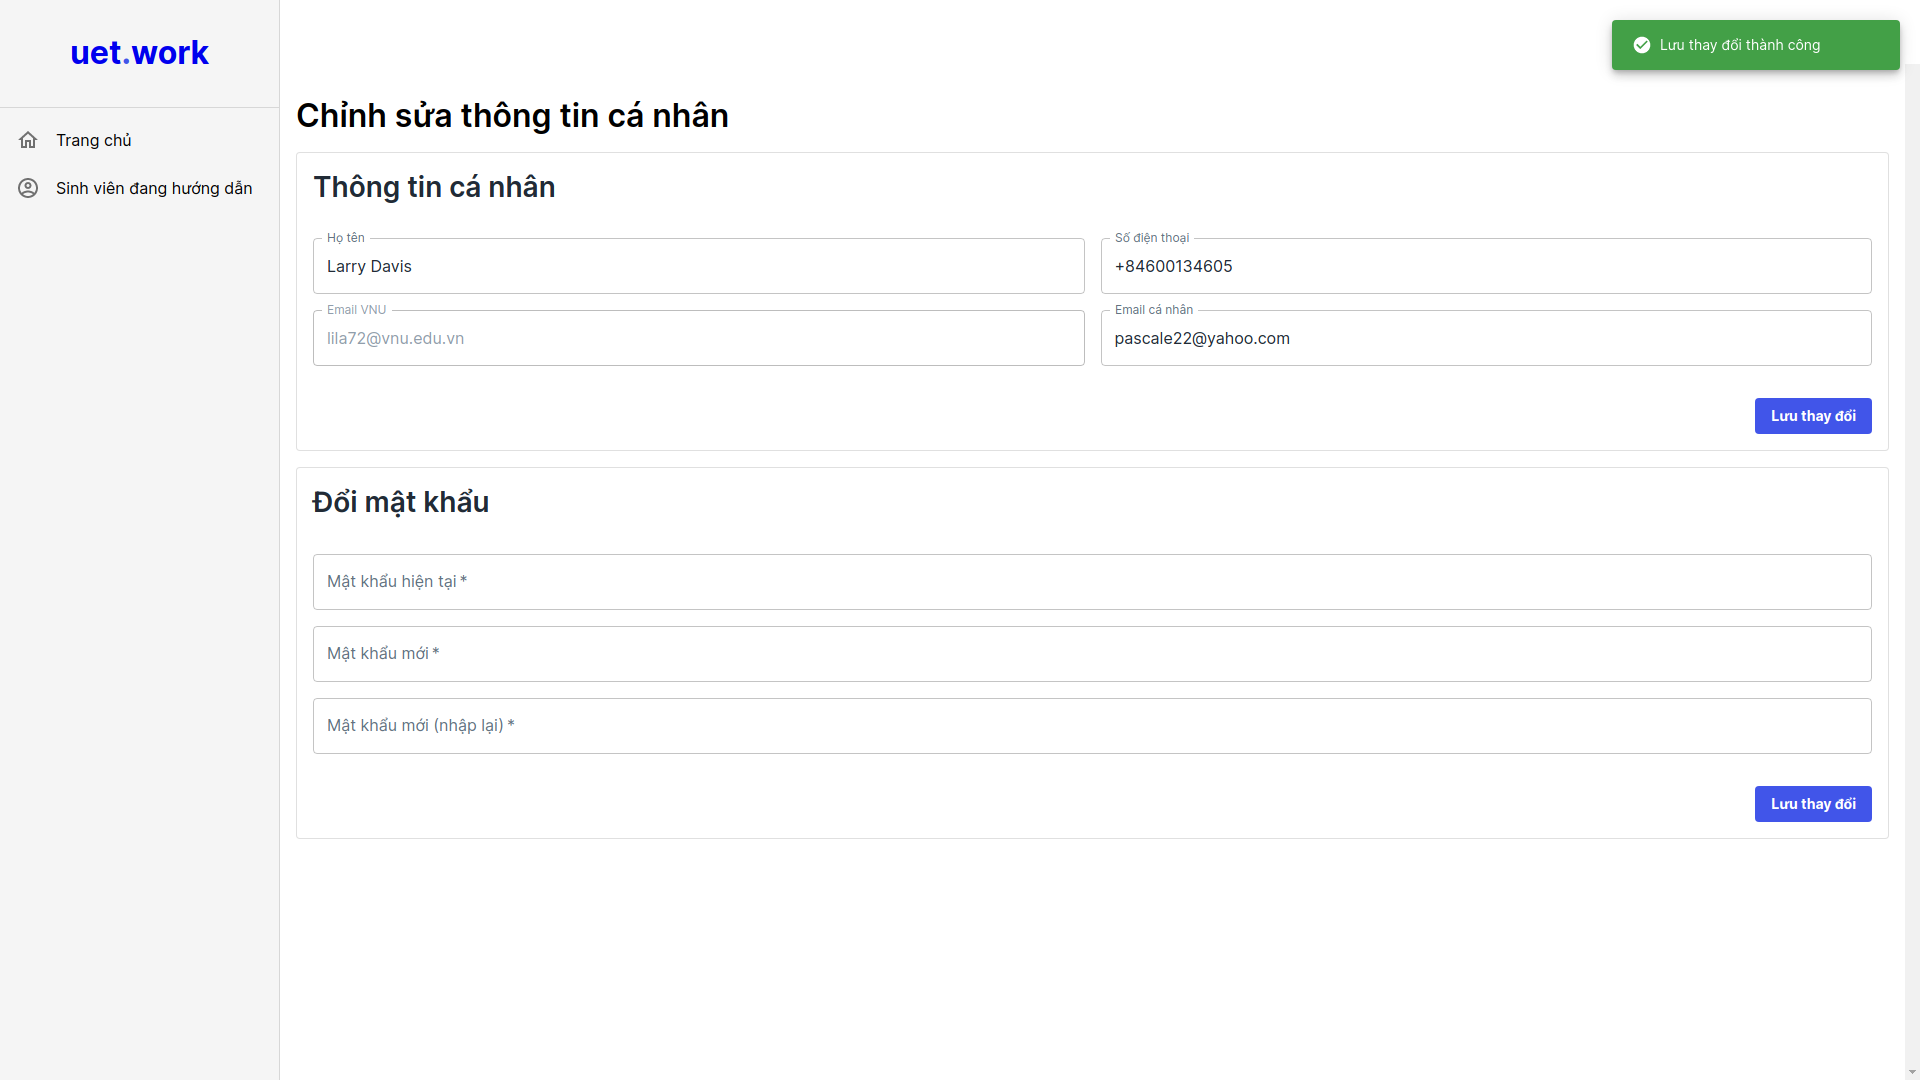
\includegraphics[width=\linewidth]{./images/image52.png}
	\caption{Luồng \emph{Giảng viên thay đổi thông tin cá nhân}: Giảng viên thay đổi thông tin cá nhân}
	\label{fig:lecturer_edit_info}
\end{figure}

\subsection{Luồng sử dụng của đối tác}

\paragraph*{Đối tác xem danh sách bài đăng}

Đối tác truy cập trang Danh sách bài đăng. Tại đây, đối tác có thể tìm kiếm, sắp xếp và lọc danh sách theo kỳ thực tập.

Hình \ref{fig:partner_list_post_page} mô tả màn hình Danh sách bài đăng của đối tác.

\begin{figure}[]
	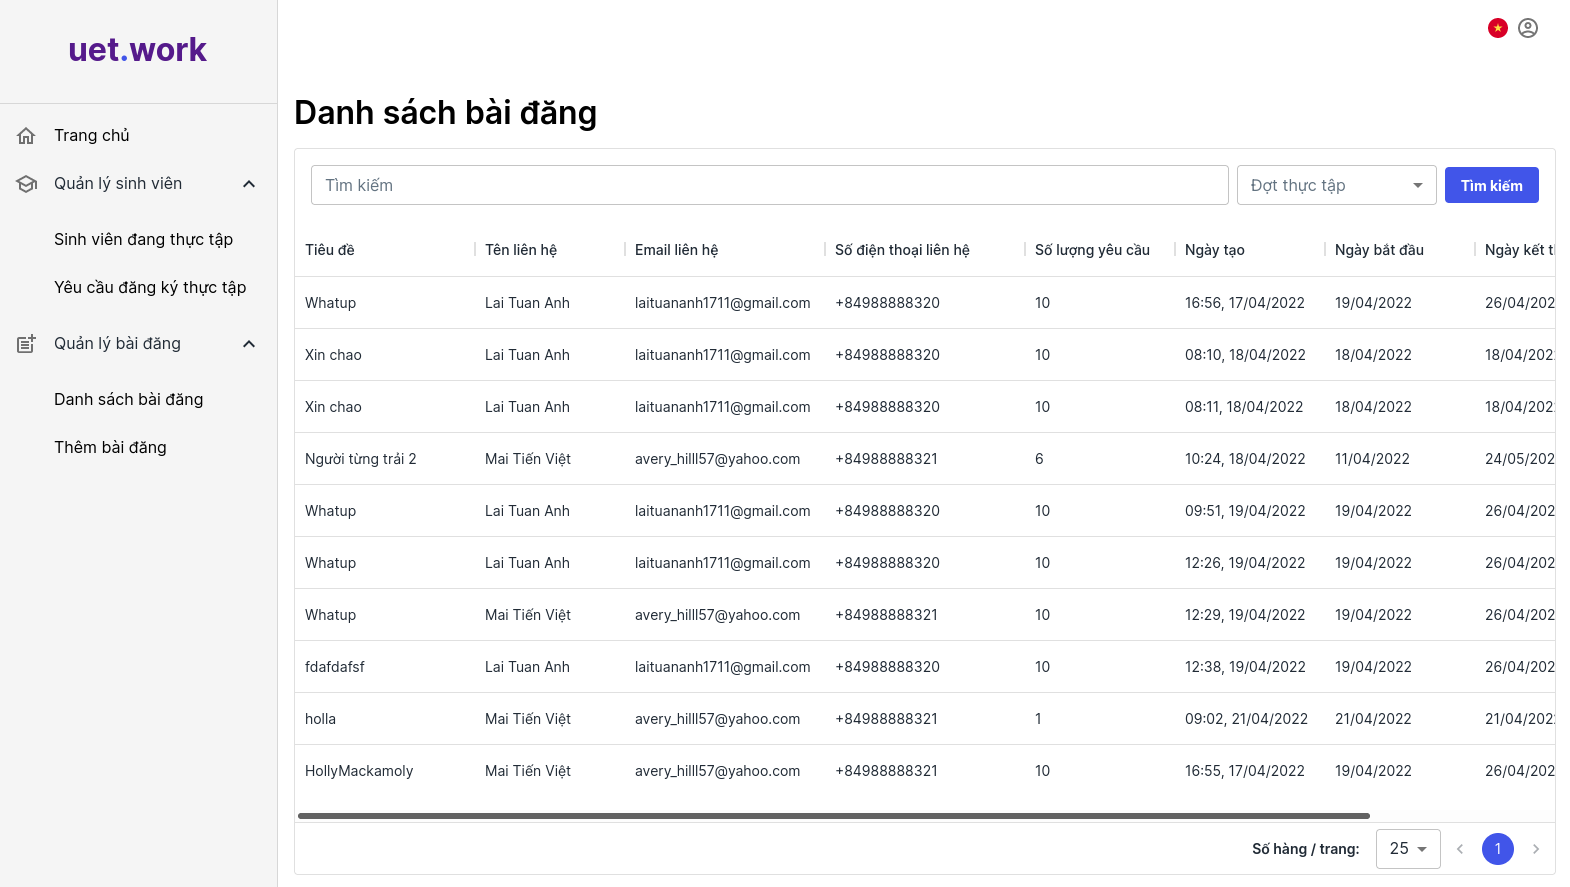
\includegraphics[width=\linewidth]{./images/list_post.png}
	\caption{Luồng \emph{Đối tác xem danh sách bài đăng}}
	\label{fig:partner_list_post_page}
\end{figure}

\paragraph*{Đối tác thêm bài đăng tuyển dụng}

Tại trang Thêm bài đăng, đối tác thêm tiêu đề, nội dung chi tiết, số lượng tuyển dụng, ngày bắt đầu, ngày kết thúc, người liên hệ để tạo một bài đăng mới.

Hình \ref{fig:add_post_page} mô tả màn hình thêm bài đăng của đối tác.

\begin{figure}[]
	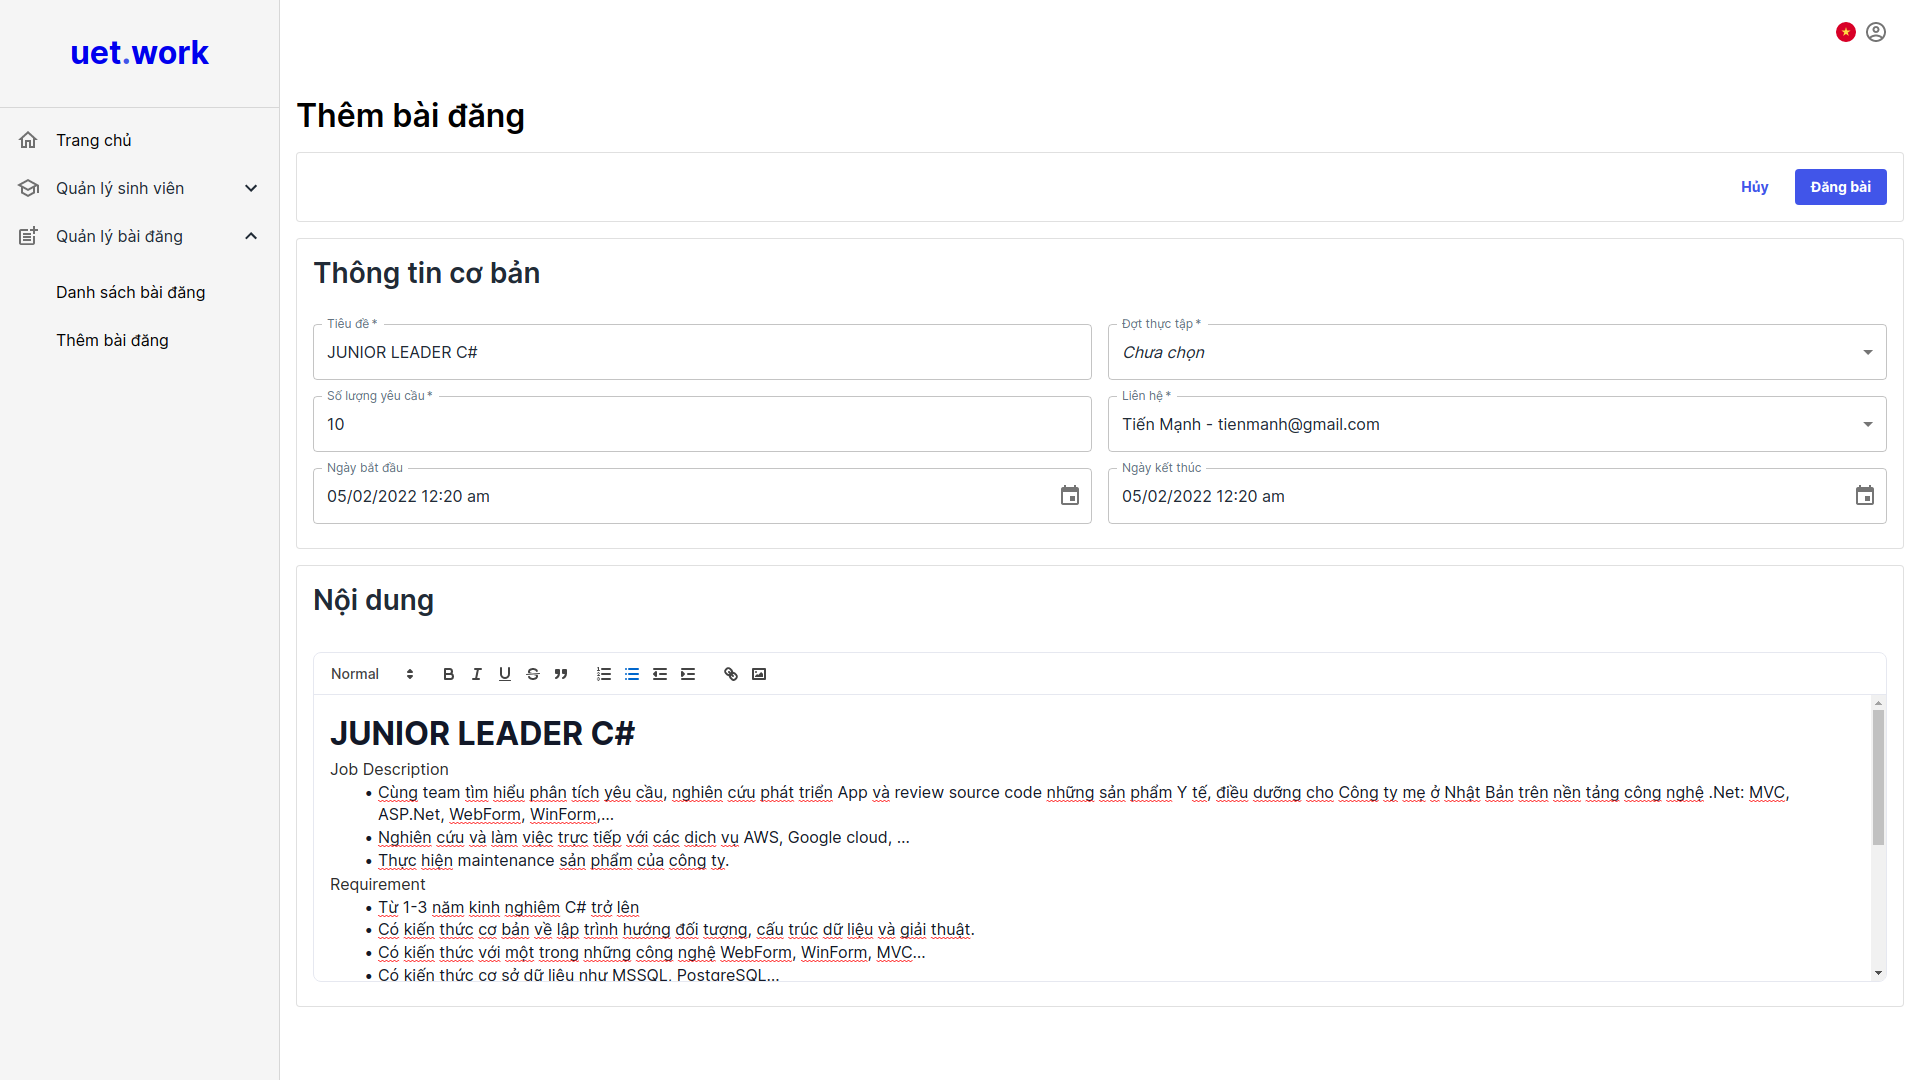
\includegraphics[width=\linewidth]{./images/image18.png}
	\caption{Luồng \emph{Đối tác thêm bài đăng tuyển dụng}}
	\label{fig:add_post_page}
\end{figure}

\paragraph*{Đối tác xem danh sách yêu cầu đăng ký thực tập}

Đối tác truy cập trang Yêu cầu đăng ký thực tập. Tại đây, đối tác có thể tìm kiếm, sắp xếp, lọc danh sách theo kỳ thực tập và chấp nhận / từ chối sinh viên.

Hình \ref{fig:partner_view_list_requests_page} mô tả màn hình danh sách yêu cầu đăng ký thực tập.

\begin{figure}[]
	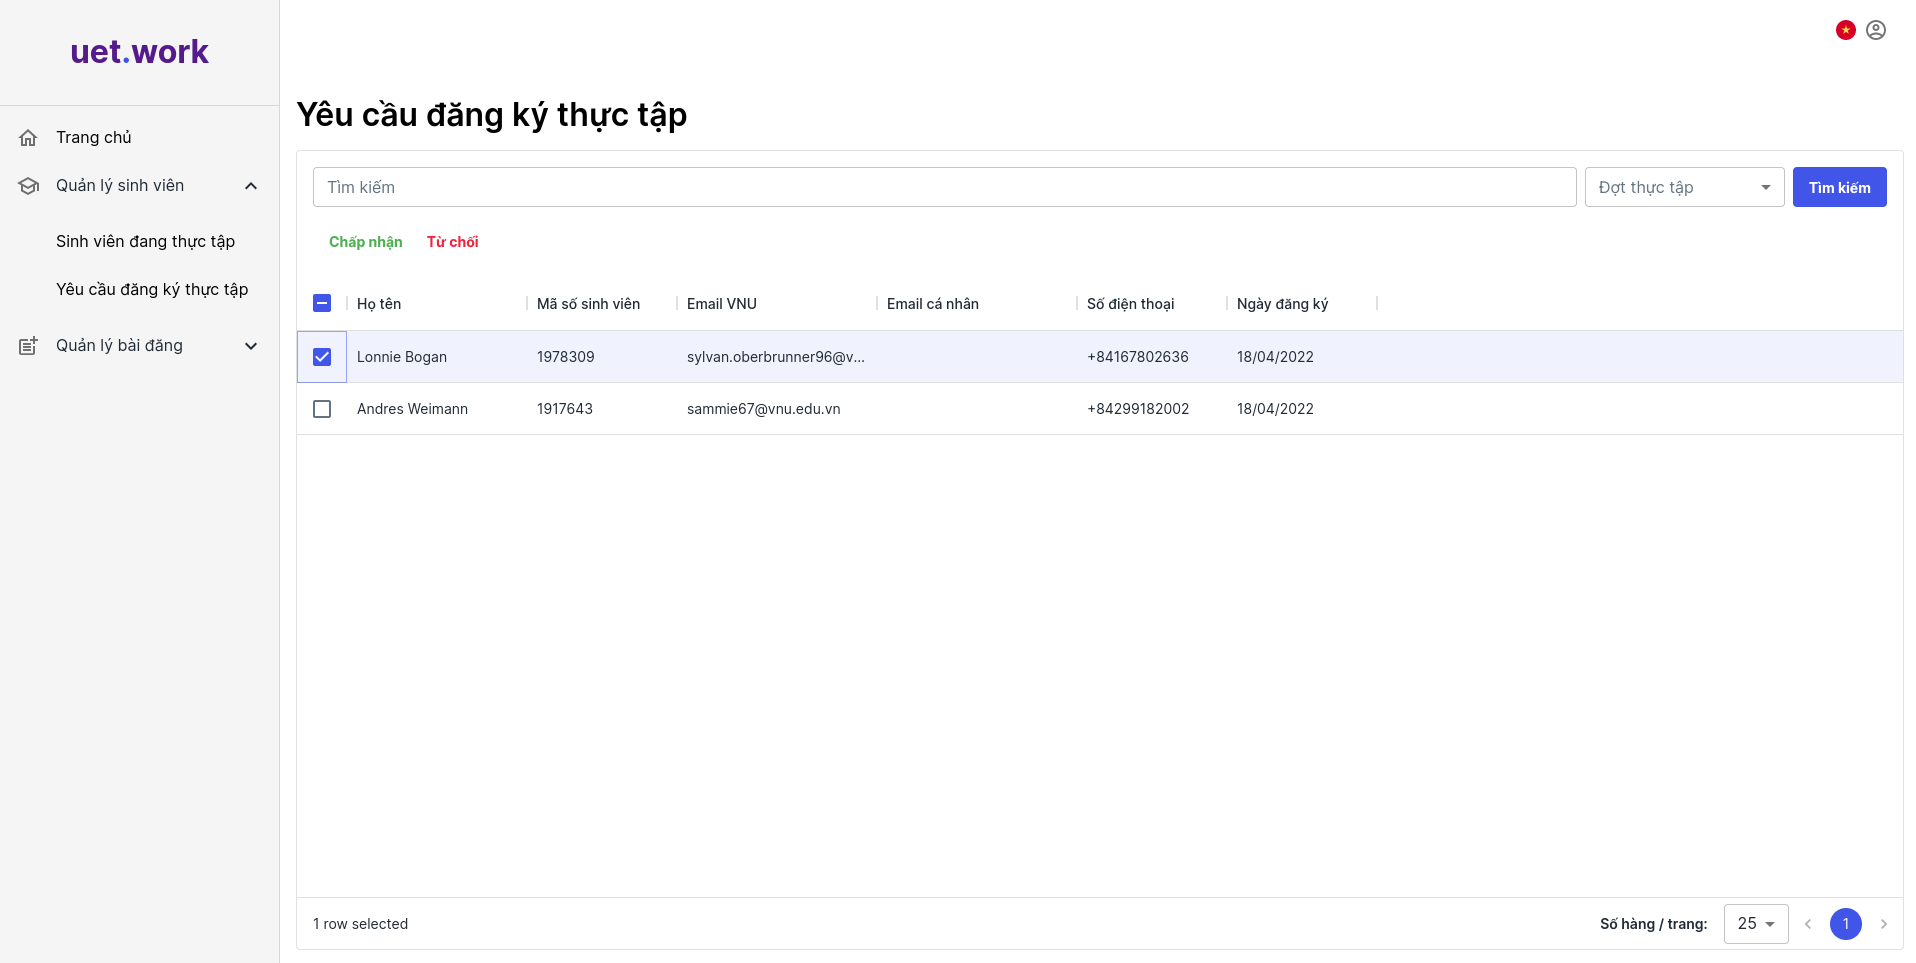
\includegraphics[width=\linewidth]{./images/image29.png}
	\caption{Luồng \emph{Đối tác xem danh sách yêu cầu đăng ký thực tập}}
	\label{fig:partner_view_list_requests_page}
\end{figure}

\paragraph*{Đối tác Chấp nhận / Từ chối yêu cầu thực tập}

\begin{itemize}
	\item Hình \ref{fig:partner_list_requests_page}: Đối tác truy cập danh sách Yêu cầu đăng ký thực tập. 
	\item Hình \ref{fig:partner_select_students_approve}: Đối tác chọn sinh viên và chọn Chấp nhận.
	\item Hình \ref{fig:partner_select_students_reject}: Đối tác chọn sinh viên và chọn Từ chối.
\end{itemize}

\begin{figure}[]
	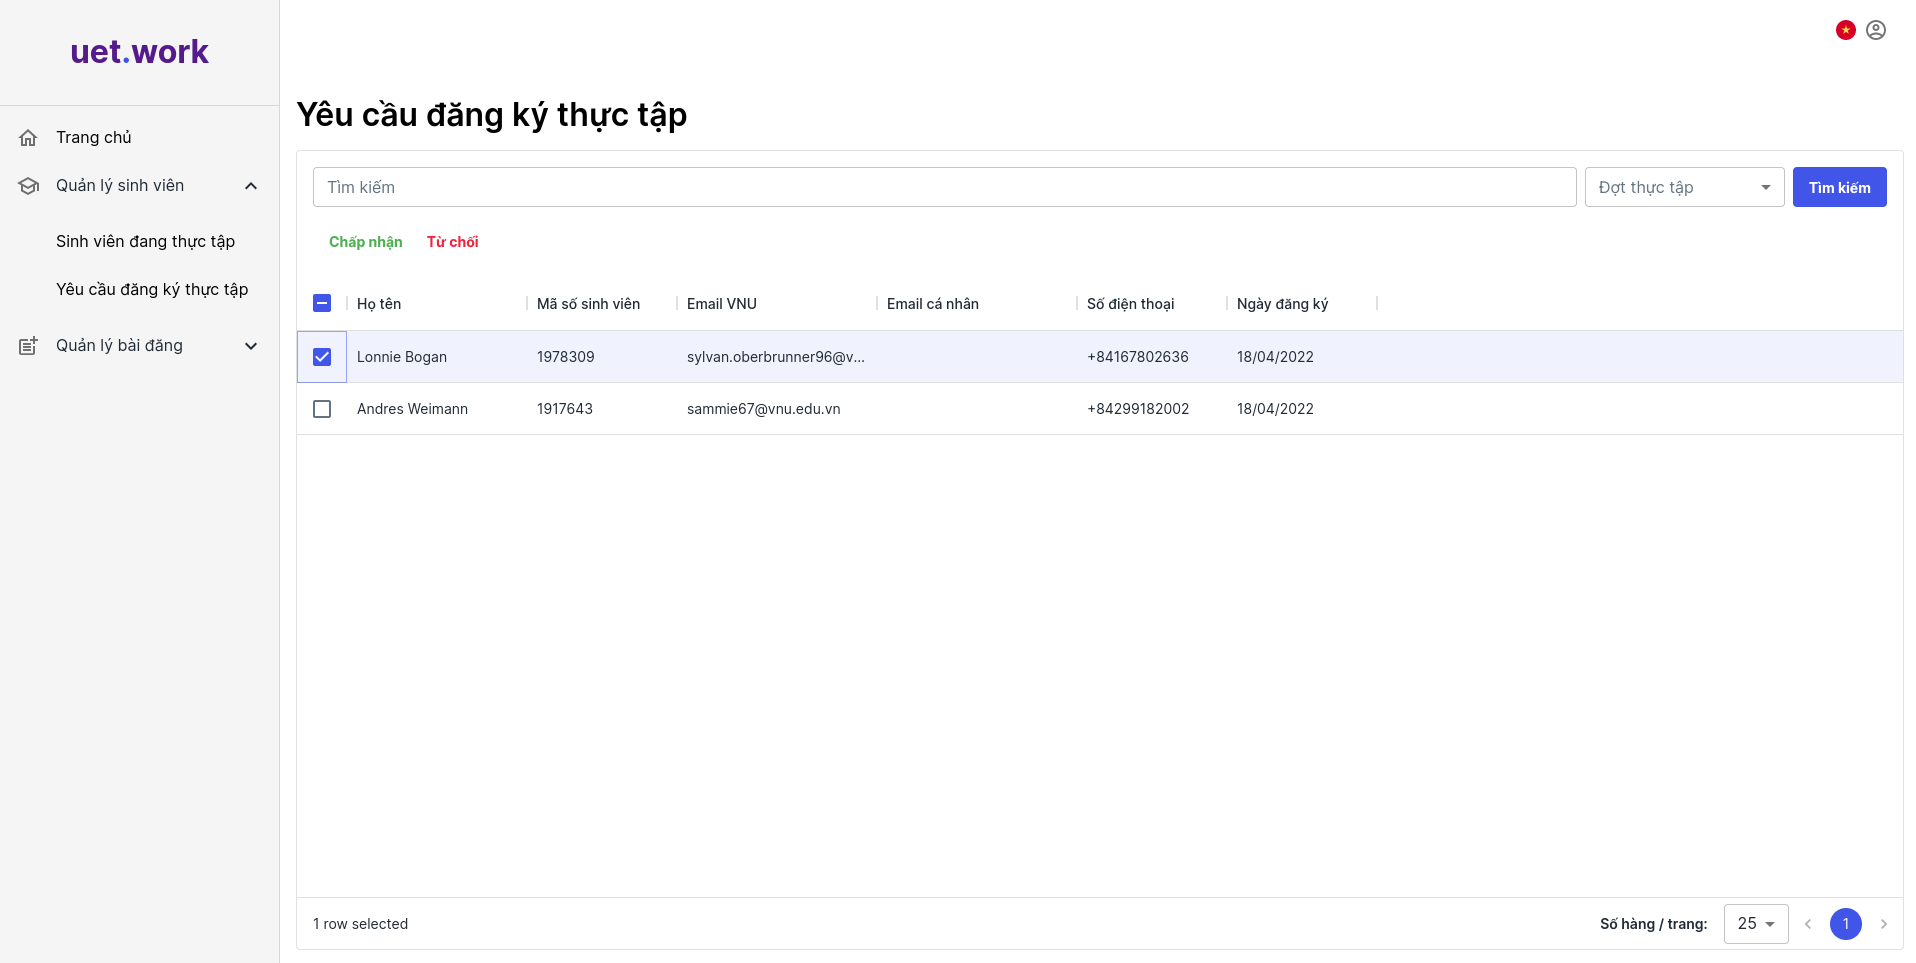
\includegraphics[width=\linewidth]{./images/image29.png}
	\caption{Luồng \emph{Đối tác Chấp nhận / Từ chối yêu cầu thực tập}: truy cập danh sách Yêu cầu đăng ký thực tập}
	\label{fig:partner_list_requests_page}
\end{figure}

\begin{figure}[]
	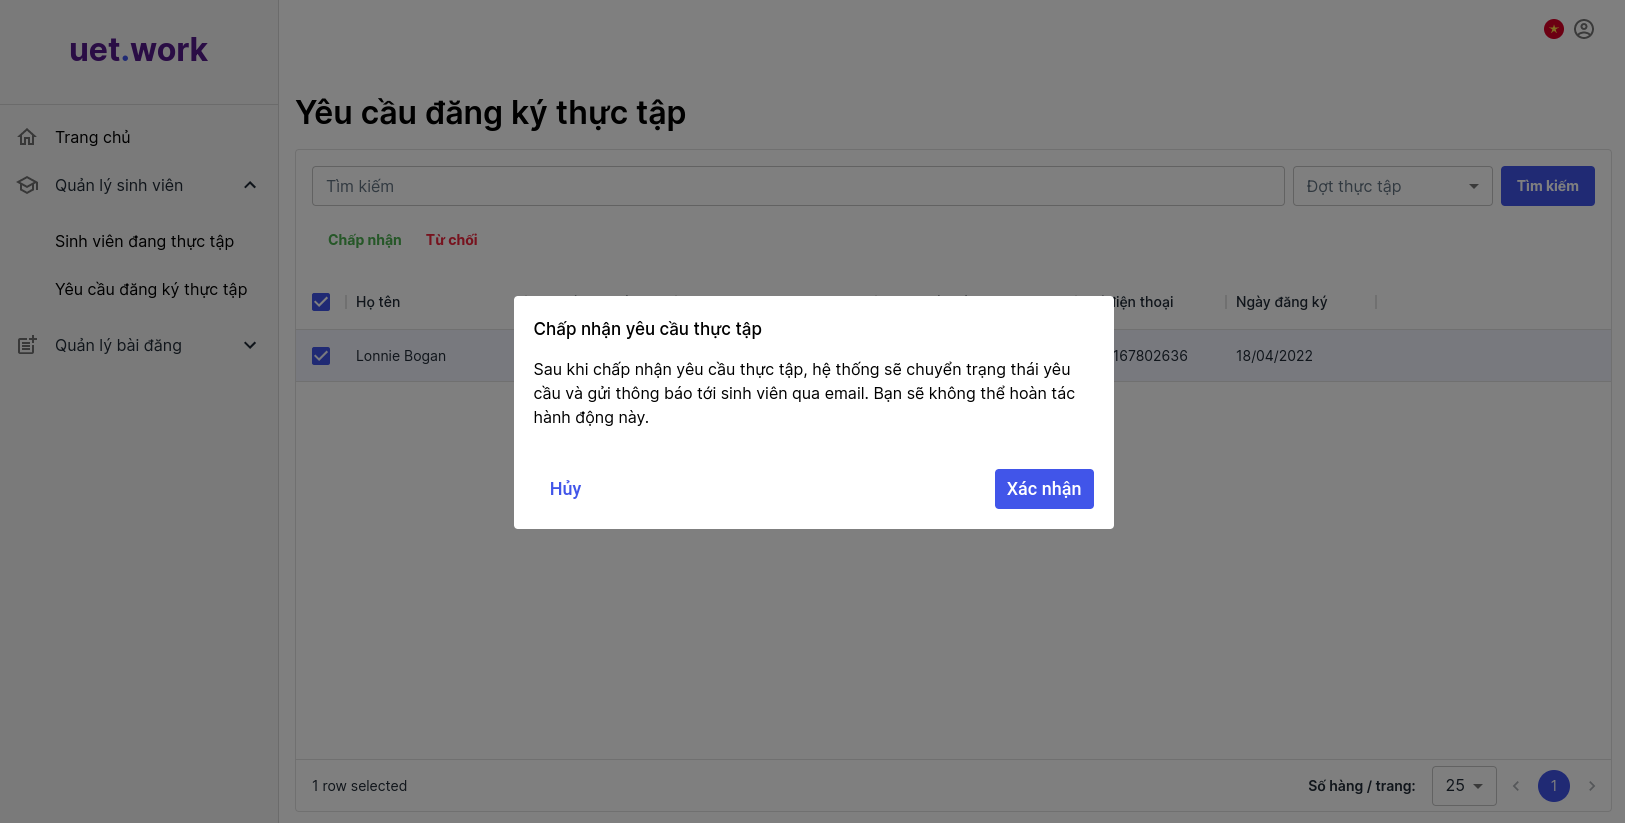
\includegraphics[width=\linewidth]{./images/image66.png}
	\caption{Luồng \emph{Đối tác chấp nhận / Từ chối yêu cầu thực tập}: chọn sinh viên và chọn Chấp nhận}
	\label{fig:partner_select_students_approve}
\end{figure}

\begin{figure}[]
	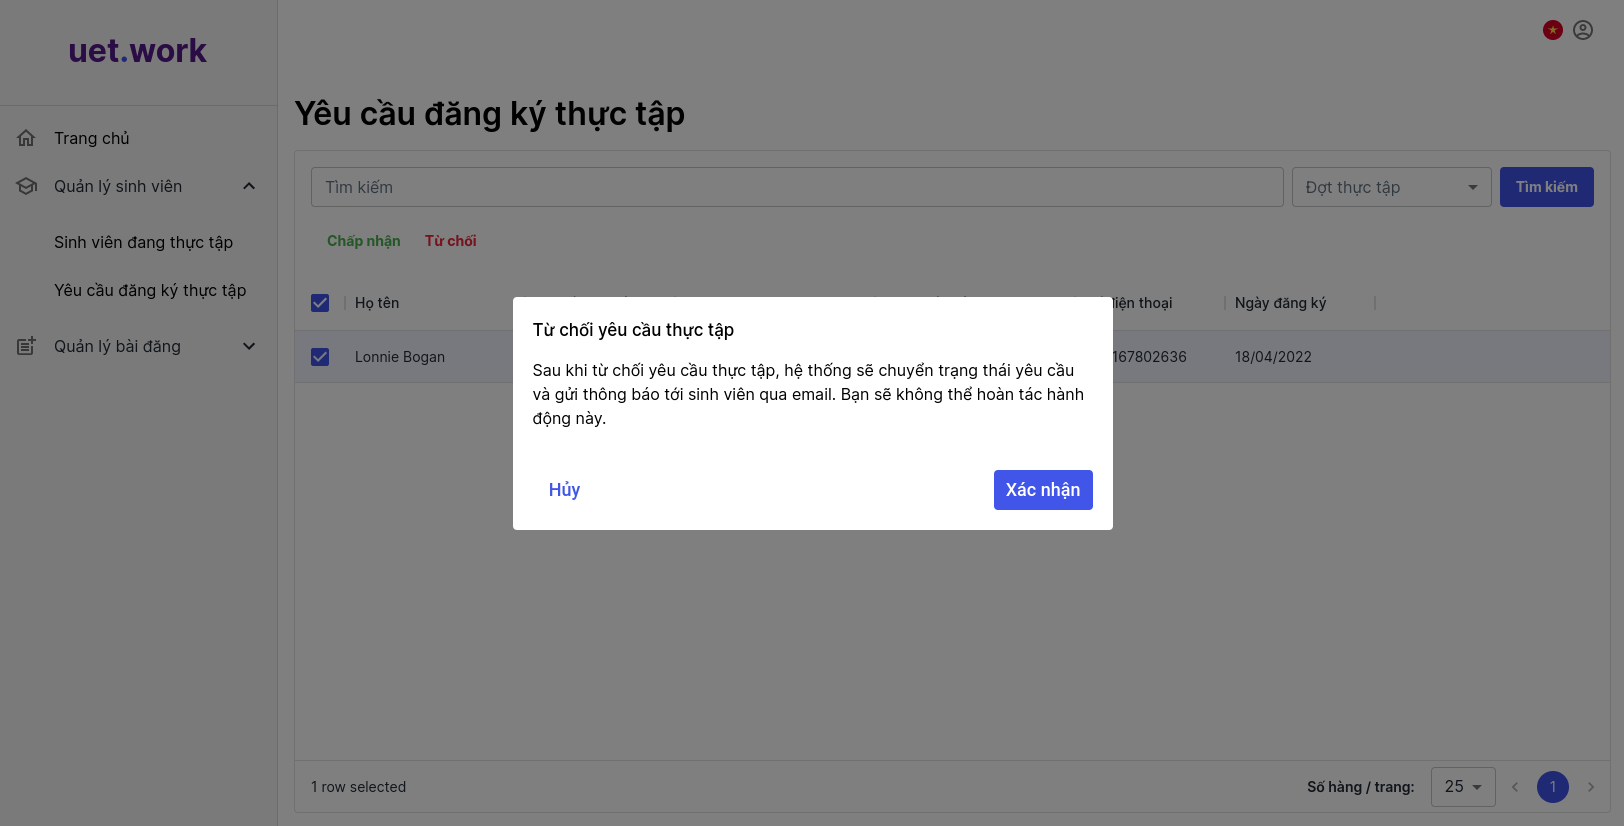
\includegraphics[width=\linewidth]{./images/image67.png}
	\caption{Luồng \emph{Đối tác Chấp nhận / Từ chối yêu cầu thực tập}: chọn sinh viên và chọn Từ chối}
	\label{fig:partner_select_students_reject}
\end{figure}

\paragraph*{Đối tác xem danh sách sinh viên đang thực tập}

Đối tác truy cập trang Sinh viên đang thực tập. Tại đây, đối tác có thể tìm kiếm, sắp xếp và lọc danh sách theo kỳ thực tập.

Hình \ref{fig:partner_view_list_working_students_page} mô tả màn hình danh sách sinh viên đang thực tập.

\begin{figure}[]
	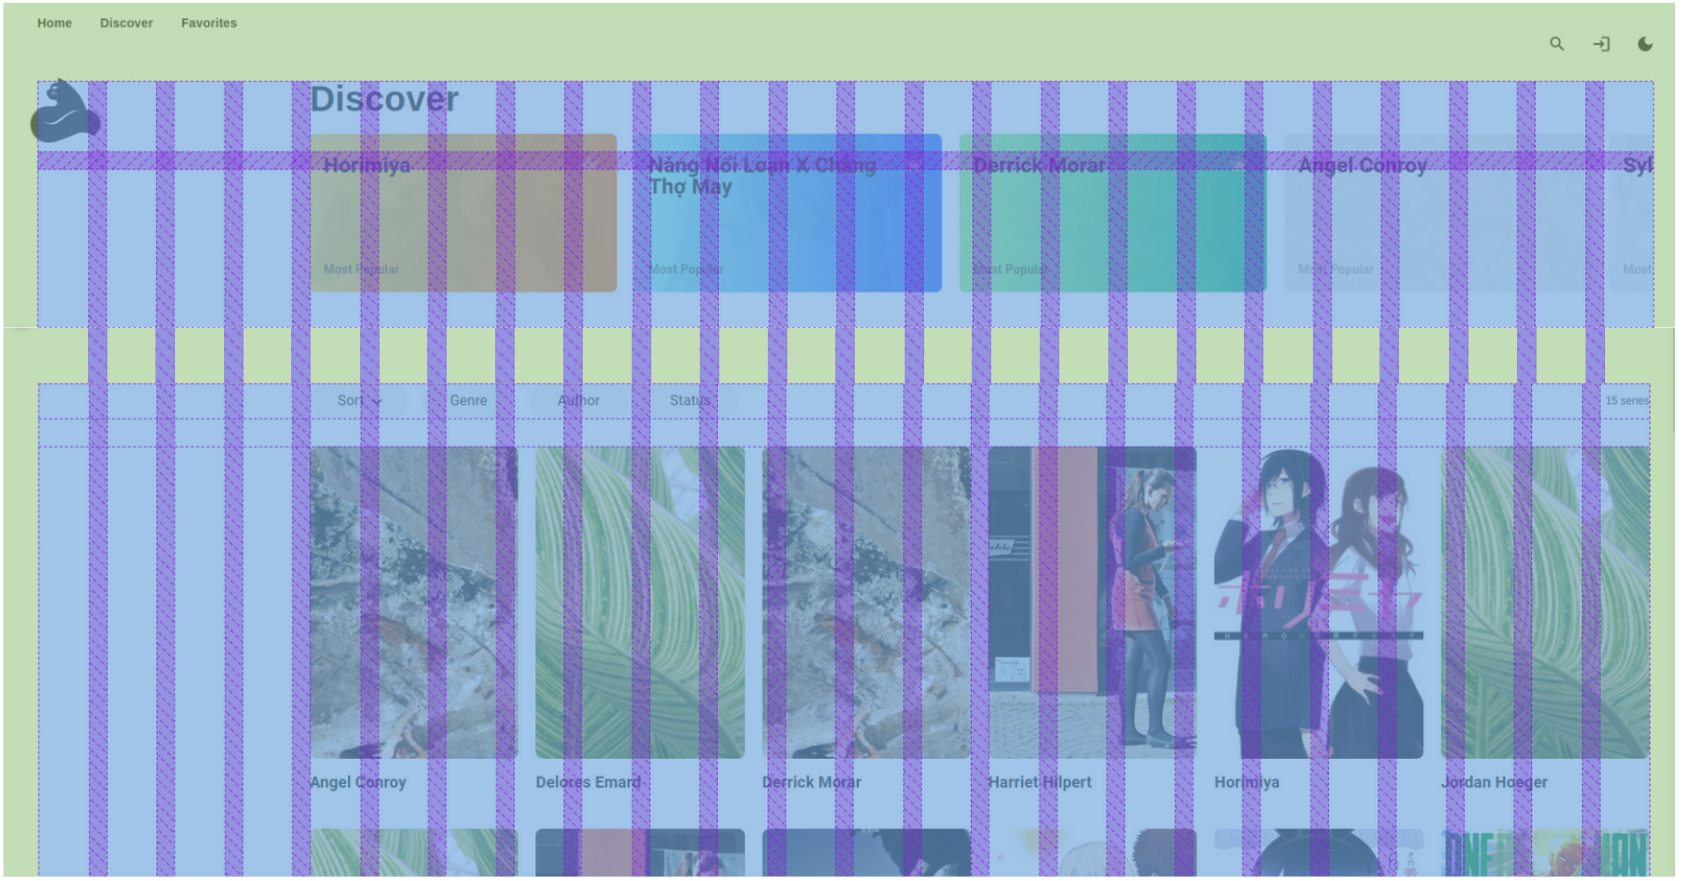
\includegraphics[width=\linewidth]{./images/image9.png}
	\caption{Luồng \emph{Đối tác xem danh sách sinh viên đang thực tập}}
	\label{fig:partner_view_list_working_students_page}
\end{figure}

\paragraph*{Đối tác sửa / thêm liên hệ}

\begin{itemize}
	\item Hình \ref{fig:partner_info_page}: Đối tác truy cập trang thông tin cá nhân. 
	\item Hình \ref{fig:partner_upsert_contact}: Đối tác Sửa/Thêm liên hệ.
\end{itemize}

\begin{figure}[]
	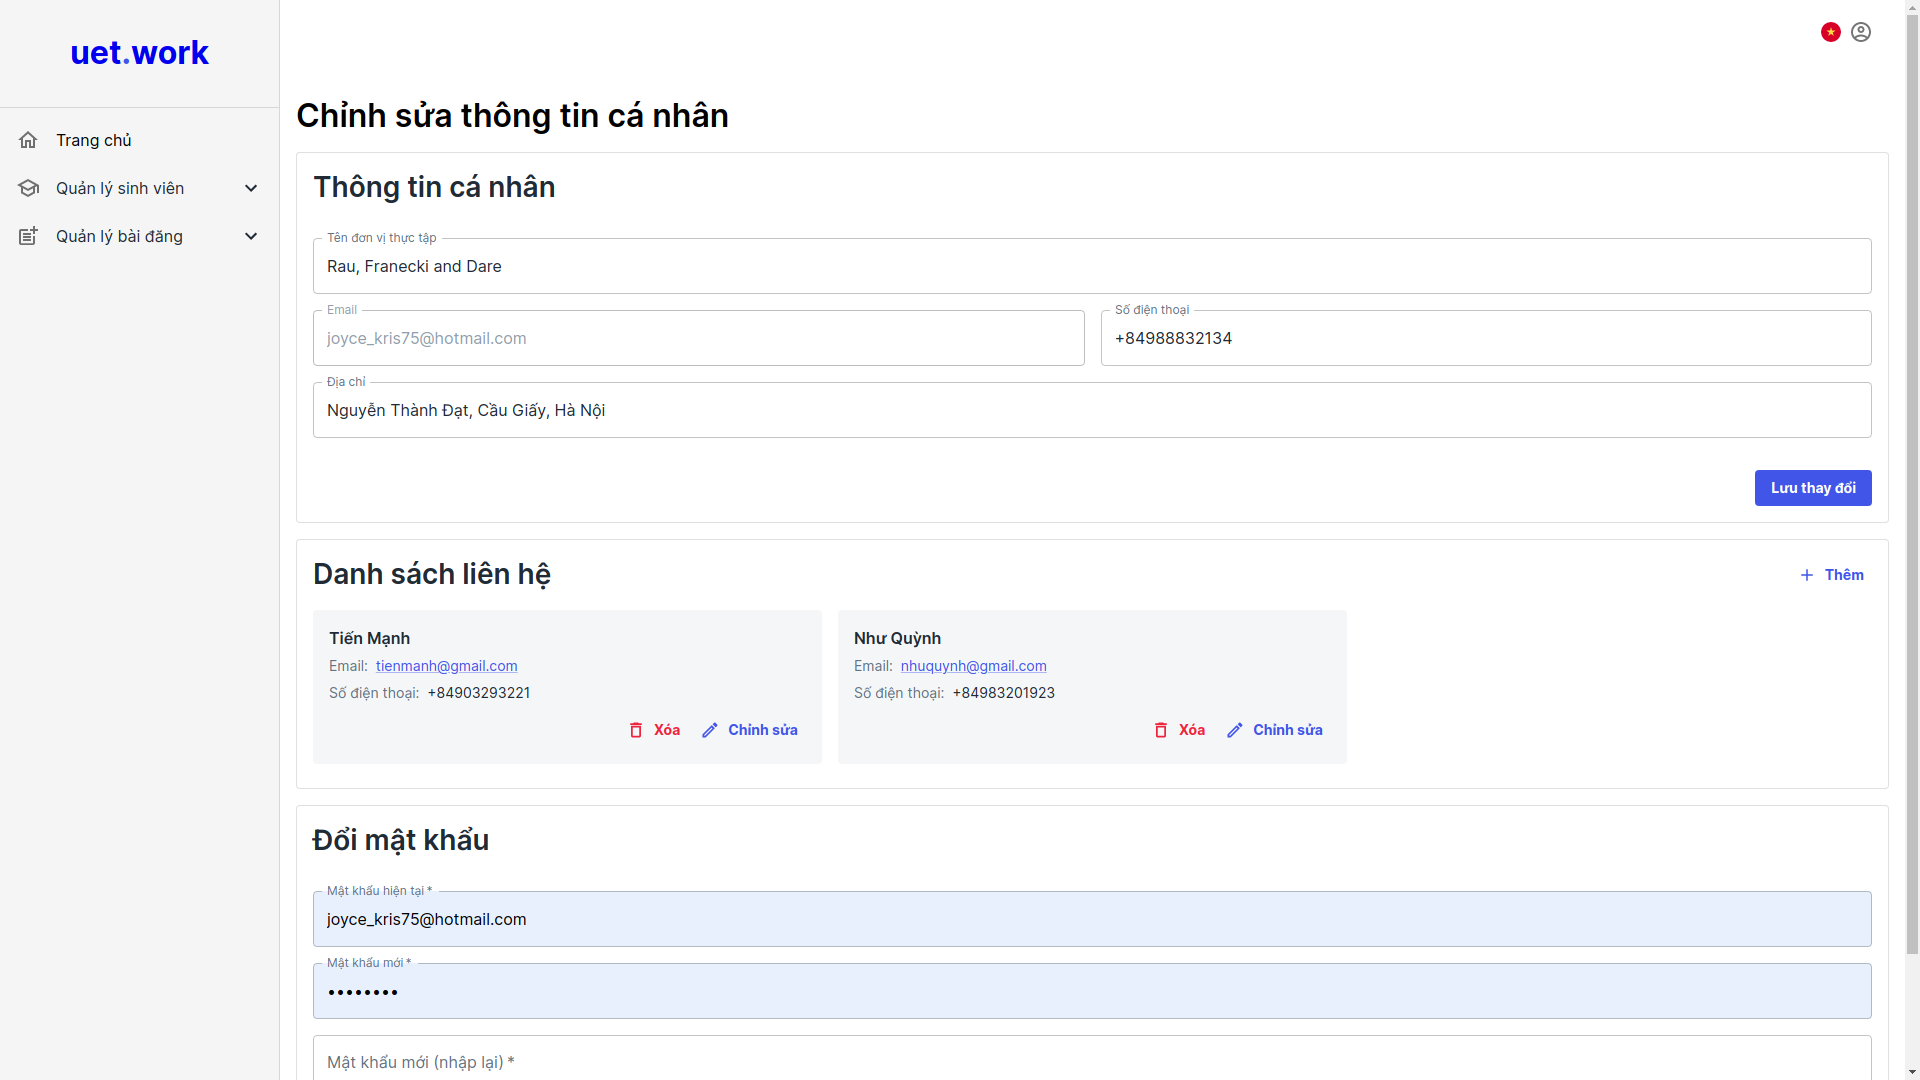
\includegraphics[width=\linewidth]{./images/image48-1.png}
	\caption{Luồng \emph{Đối tác sửa / thêm liên hệ}: Truy cập trang thông tin cá nhân}
	\label{fig:partner_info_page}
\end{figure}

\begin{figure}[]
	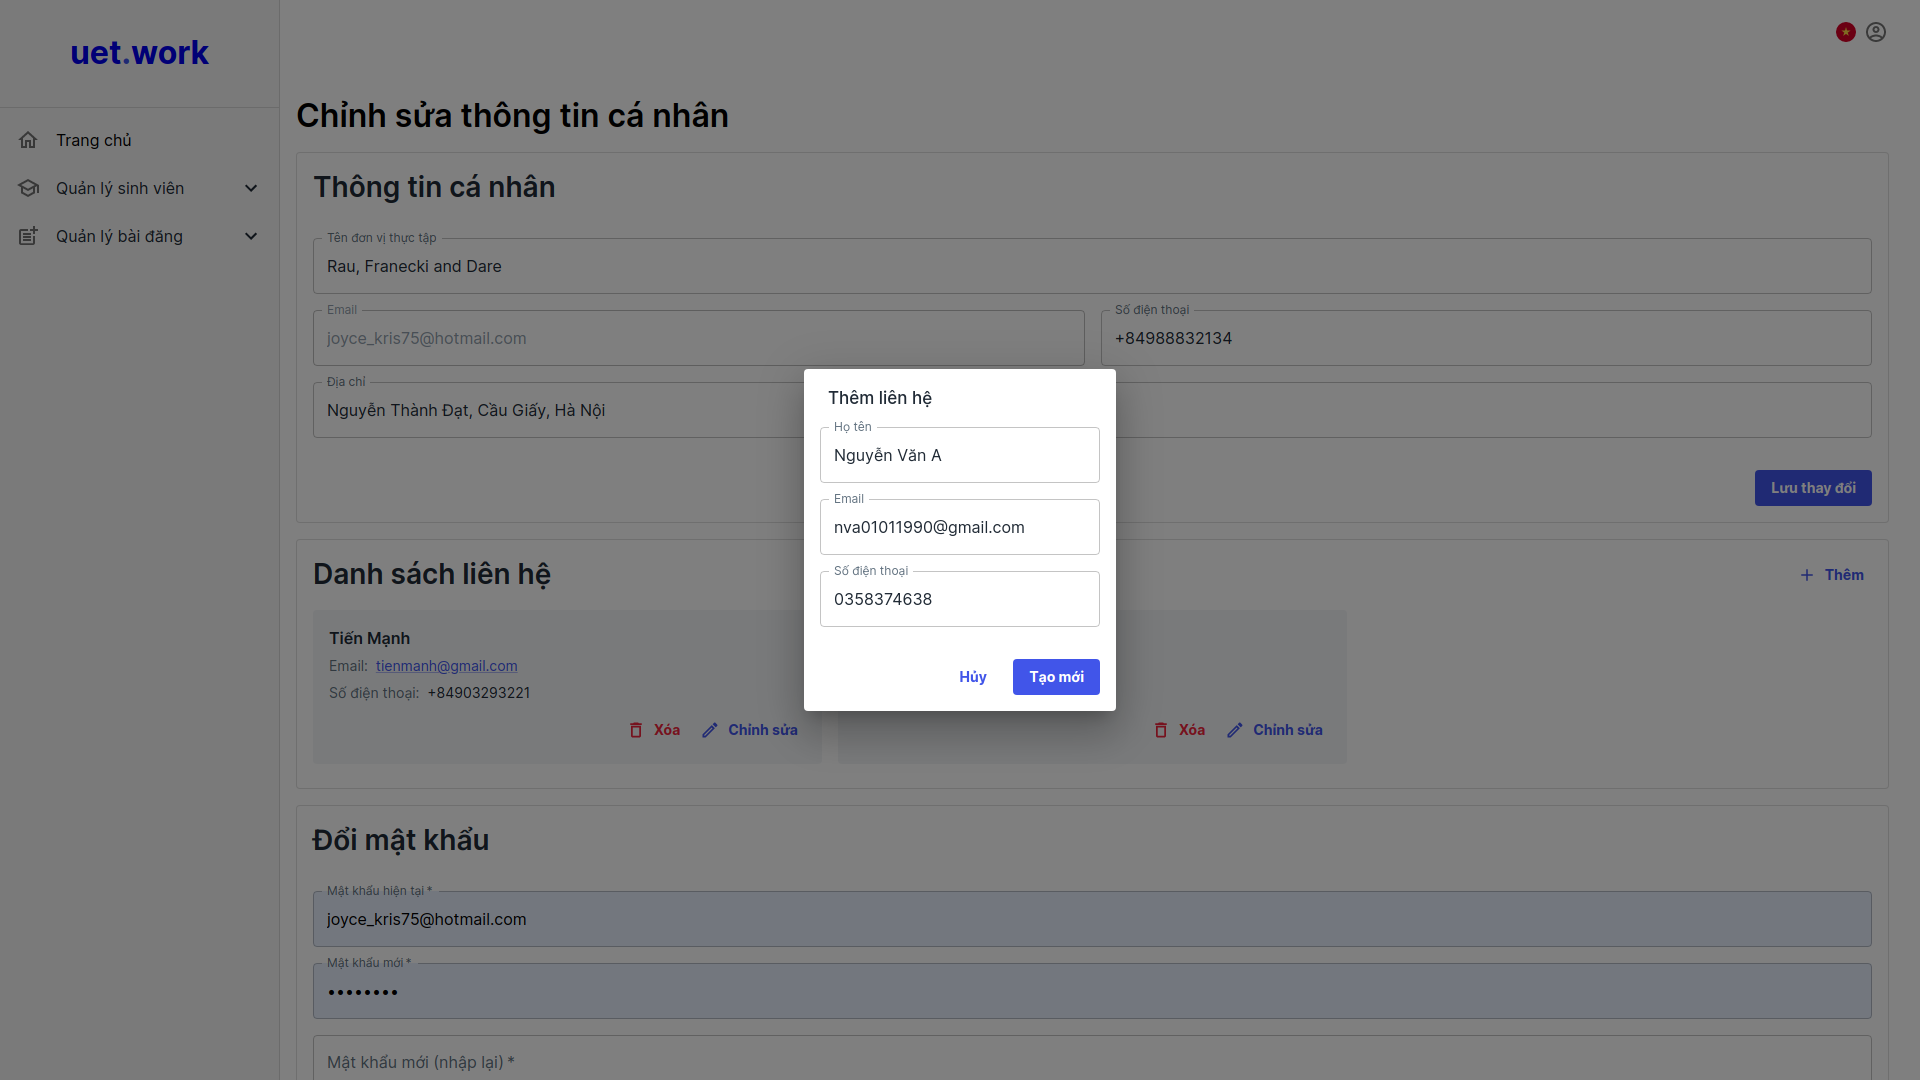
\includegraphics[width=\linewidth]{./images/image48.png}
	\caption{Luồng \emph{Đối tác sửa / thêm liên hệ}: Sửa/Thêm liên hệ}
	\label{fig:partner_upsert_contact}
\end{figure}

\subsection{Luồng sử dụng của quản trị viên Khoa}

\paragraph*{Quản trị viên Khoa tạo kỳ thực tập mới}

\begin{itemize}
	\item Hình \ref{fig:org_admin_access_list_terms}: Quản trị viên Khoa truy cập trang Danh sách kỳ thực tập. 
	\item Hình \ref{fig:org_admin_add_term}: Quản trị viên Khoa thực hiện tạo kỳ thực tập mới.
	\item Hình \ref{fig:org_admin_add_term_success}: Tạo kỳ thực tập thành công.
\end{itemize}

\begin{figure}[]
	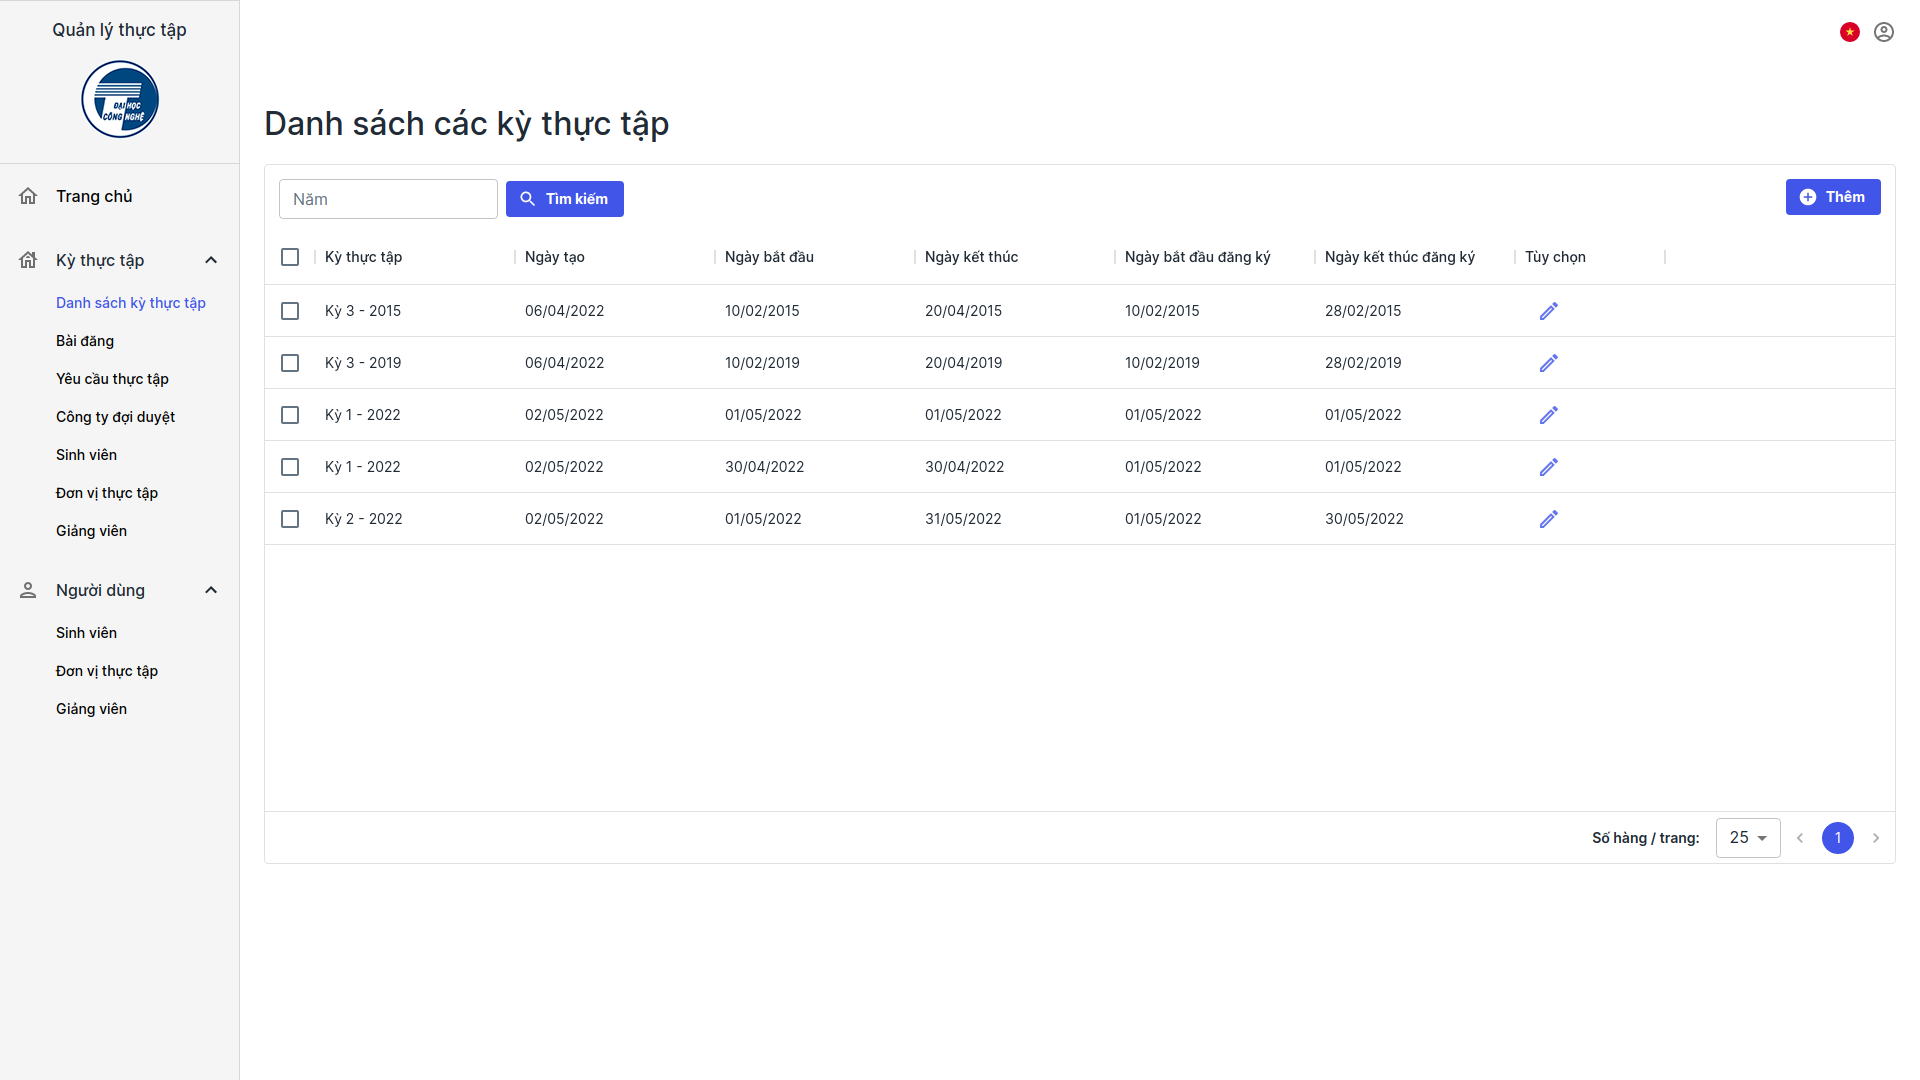
\includegraphics[width=\linewidth]{./images/image53.png}
	\caption{Luồng \emph{Quản trị viên Khoa tạo kỳ thực tập mới}: Truy cập trang Danh sách kỳ thực tập}
	\label{fig:org_admin_access_list_terms}
\end{figure}

\begin{figure}[]
	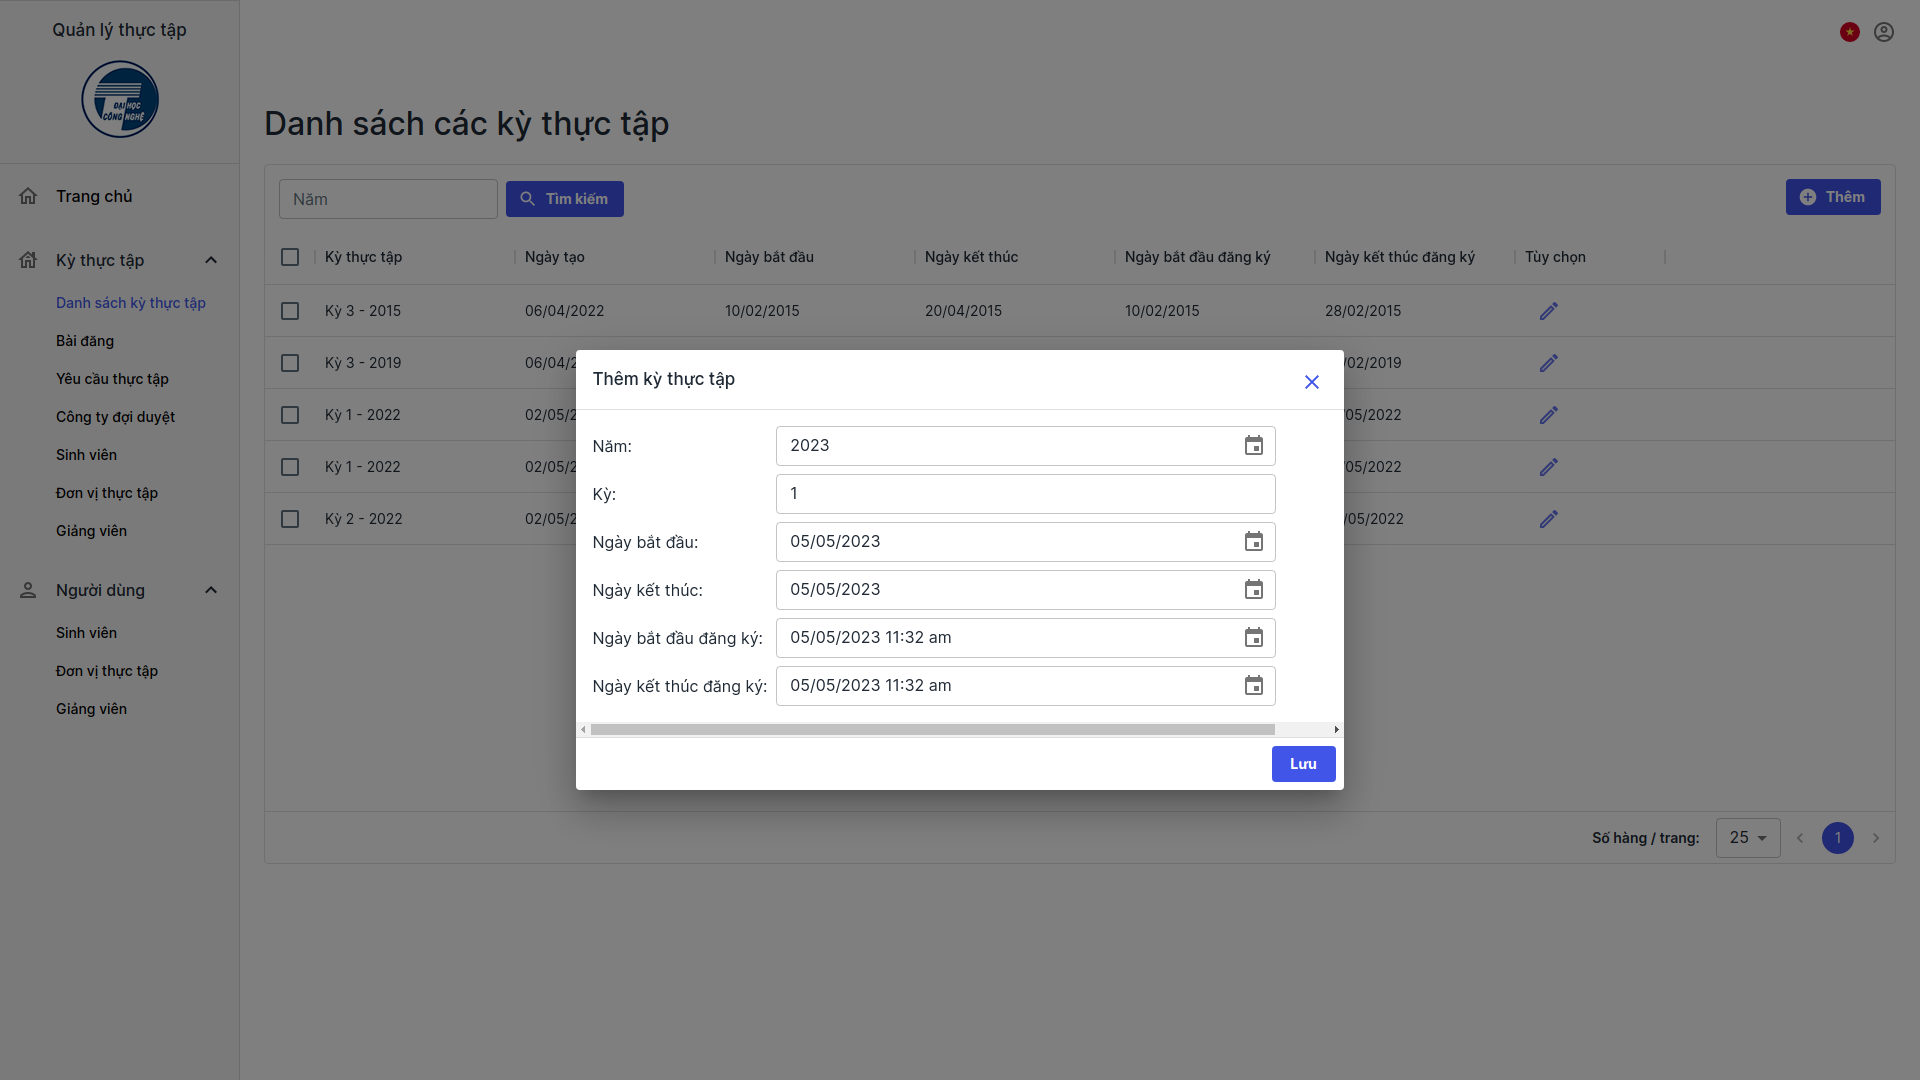
\includegraphics[width=\linewidth]{./images/image54.png}
	\caption{Luồng \emph{Quản trị viên Khoa tạo kỳ thực tập mới}: Thực hiện tạo kỳ thực tập mới}
	\label{fig:org_admin_add_term}
\end{figure}

\begin{figure}[]
	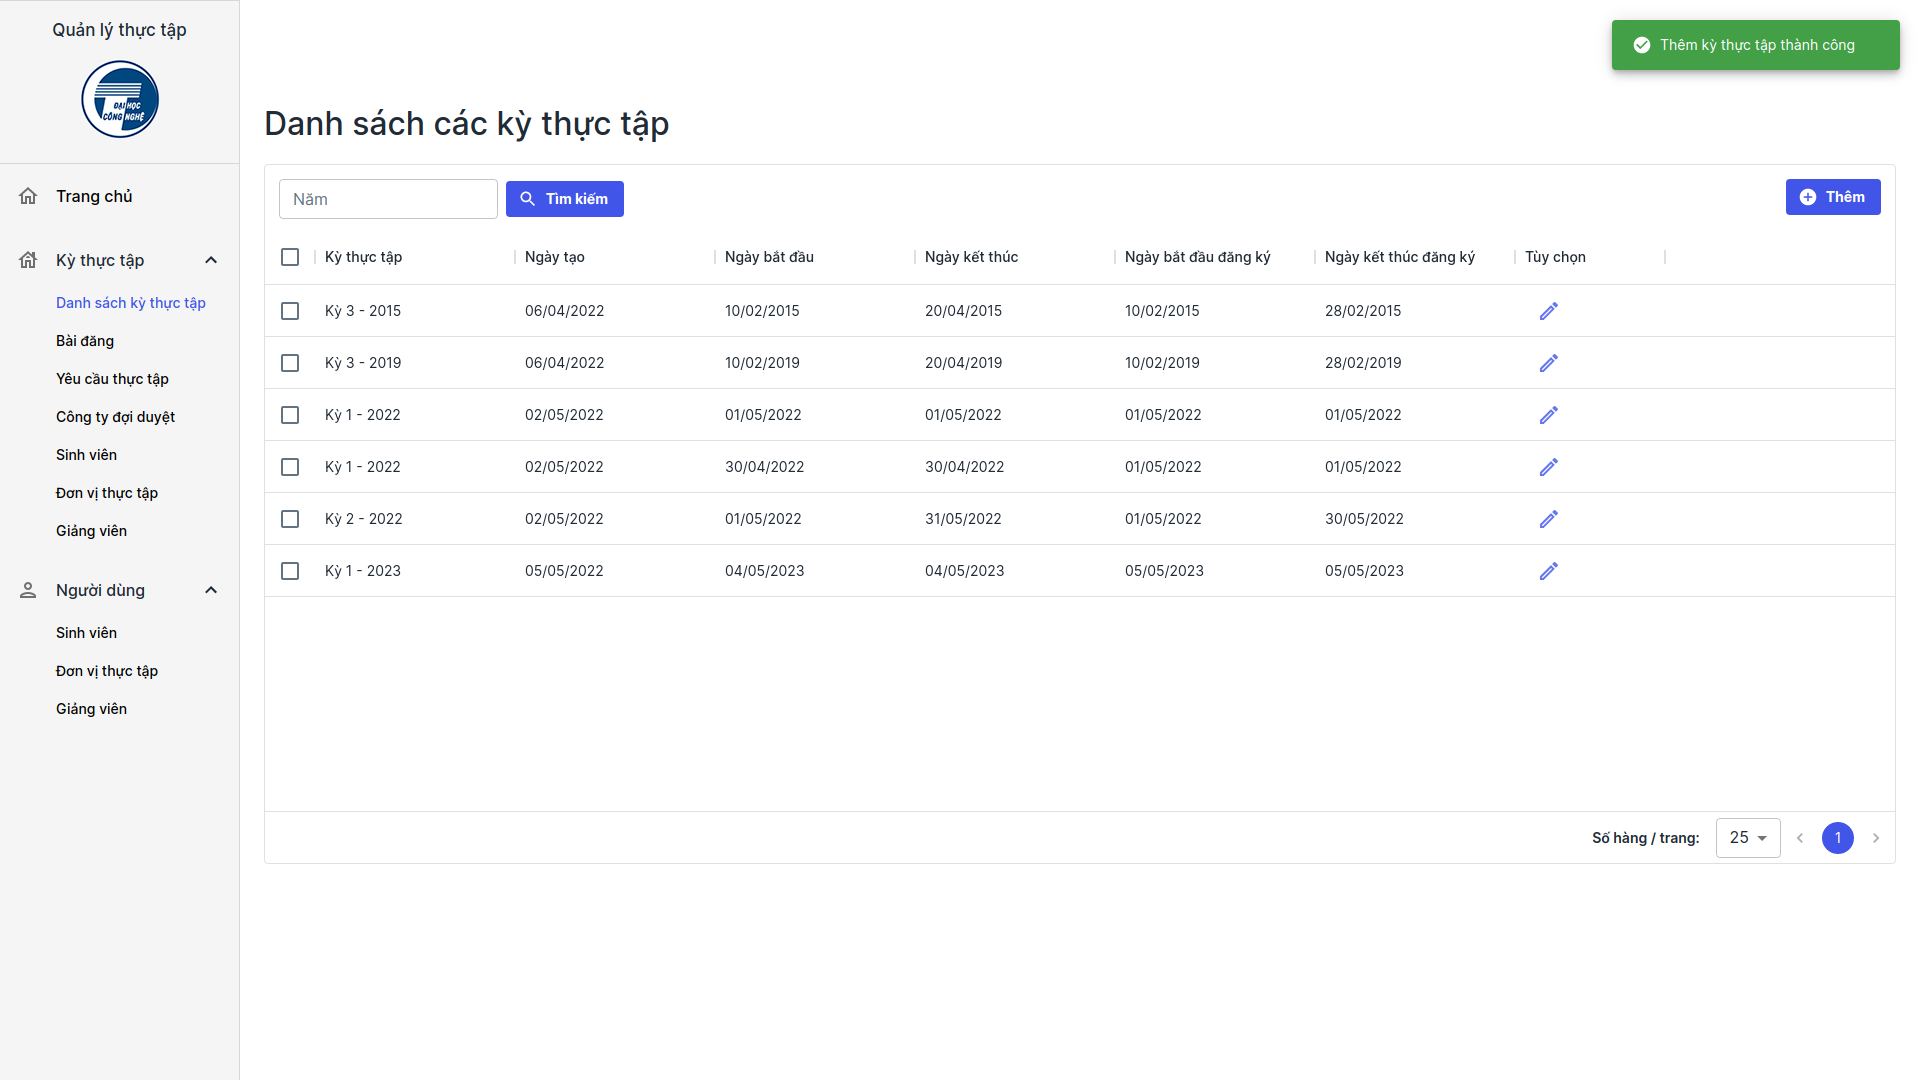
\includegraphics[width=\linewidth]{./images/image55.png}
	\caption{Luồng \emph{Quản trị viên Khoa tạo kỳ thực tập mới}: Tạo kỳ thực tập thành công}
	\label{fig:org_admin_add_term_success}
\end{figure}

\paragraph*{Quản trị viên Khoa xem danh sách bài đăng của các đối tác}

Quản trị viên truy cập trang danh sách Bài đăng. Tại đây, quản trị viên có thể tìm kiếm, sắp xếp danh sách, thêm, sửa bài đăng cho đối tác.

Hình \ref{fig:orgadmin_list_posts} mô tả màn hình danh sách bài đăng của các đối tác.

\begin{figure}[]
	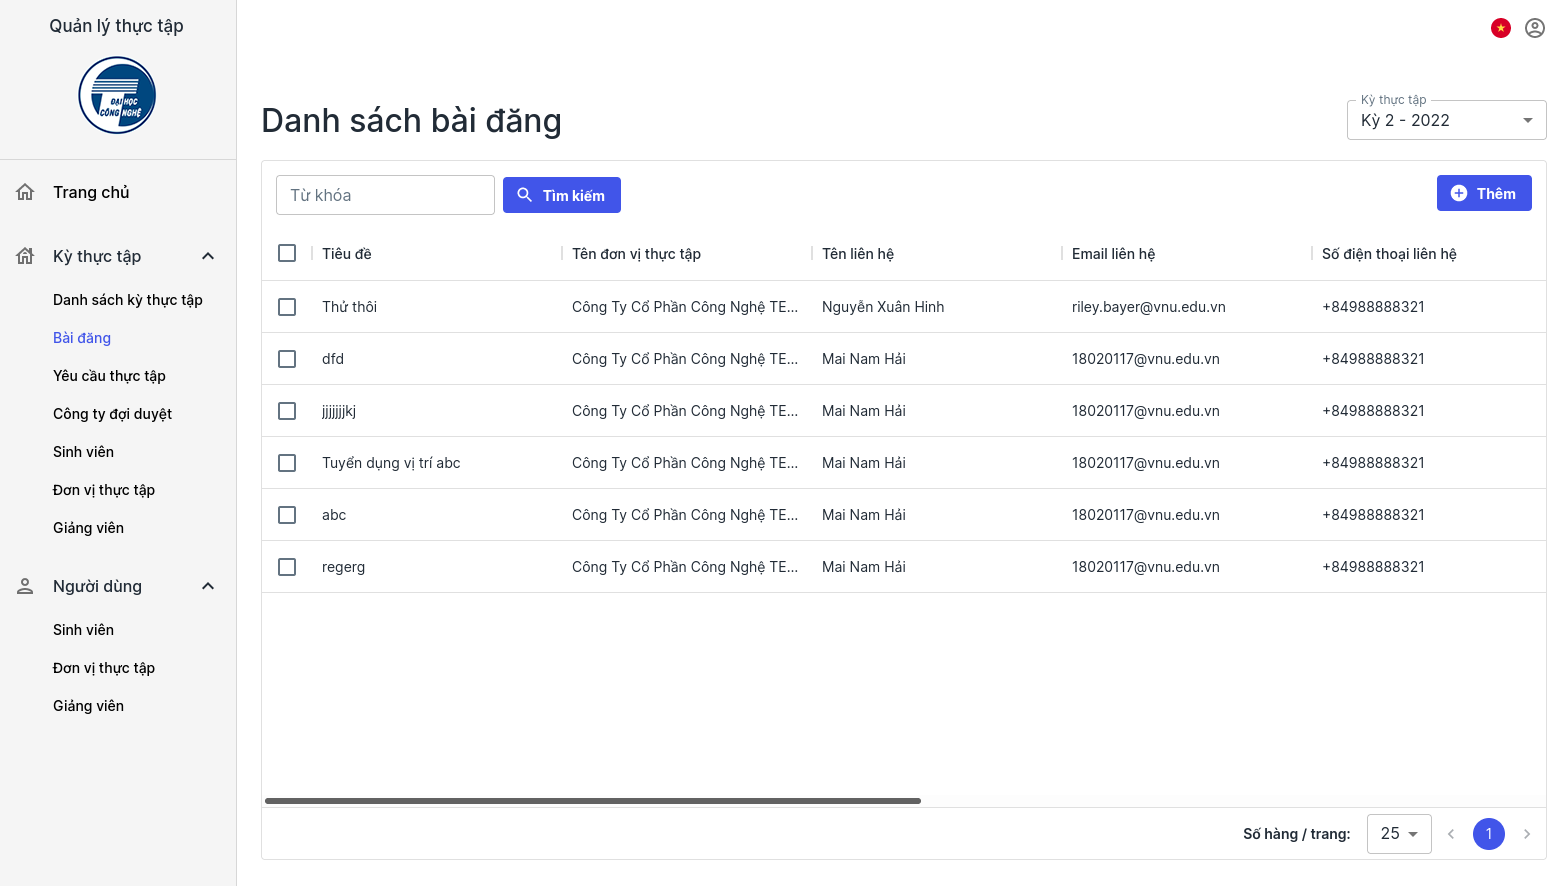
\includegraphics[width=\linewidth]{./images/image71.png}
	\caption{Luồng \emph{Quản trị viên Khoa xem danh sách bài đăng của các đối tác}}
	\label{fig:orgadmin_list_posts}
\end{figure}

\paragraph*{Quản trị viên Khoa chấp nhận / từ chối yêu cầu thực tập}

\begin{itemize}
	\item Hình \ref{fig:org_admin_access_list_requests}: Quản trị viên truy cập trang Yêu cầu thực tập trong kỳ thực tập. 
	\item Hình \ref{fig:org_admin_select_requests}: Quản trị viên chọn danh sách sinh viên và chọn tùy chọn Chấp nhận / Từ chối.
\end{itemize}

\begin{figure}[]
	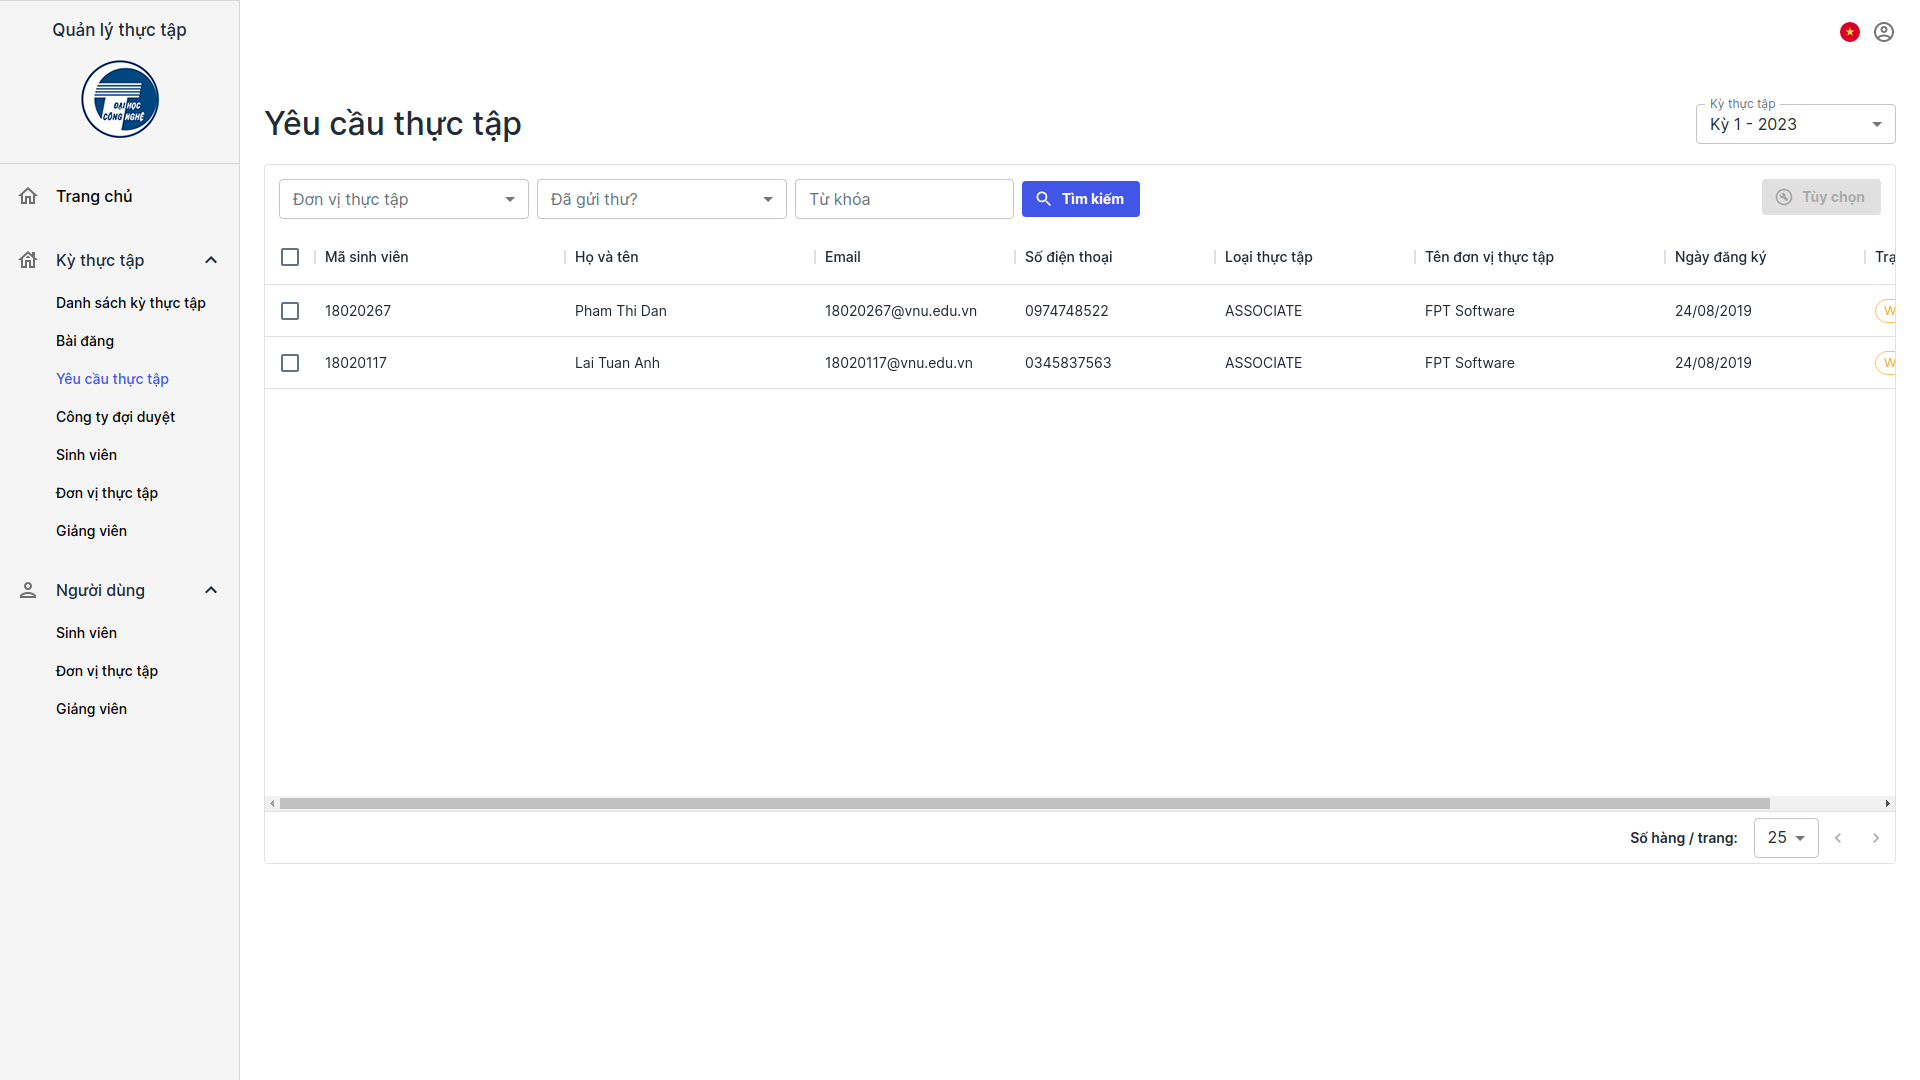
\includegraphics[width=\linewidth]{./images/image72.png}
	\caption{Luồng \emph{Quản trị viên Khoa Chấp nhận / từ chối yêu cầu thực tập}: truy cập danh sách yêu cầu thực tập}
	\label{fig:org_admin_access_list_requests}
\end{figure}

\begin{figure}[]
	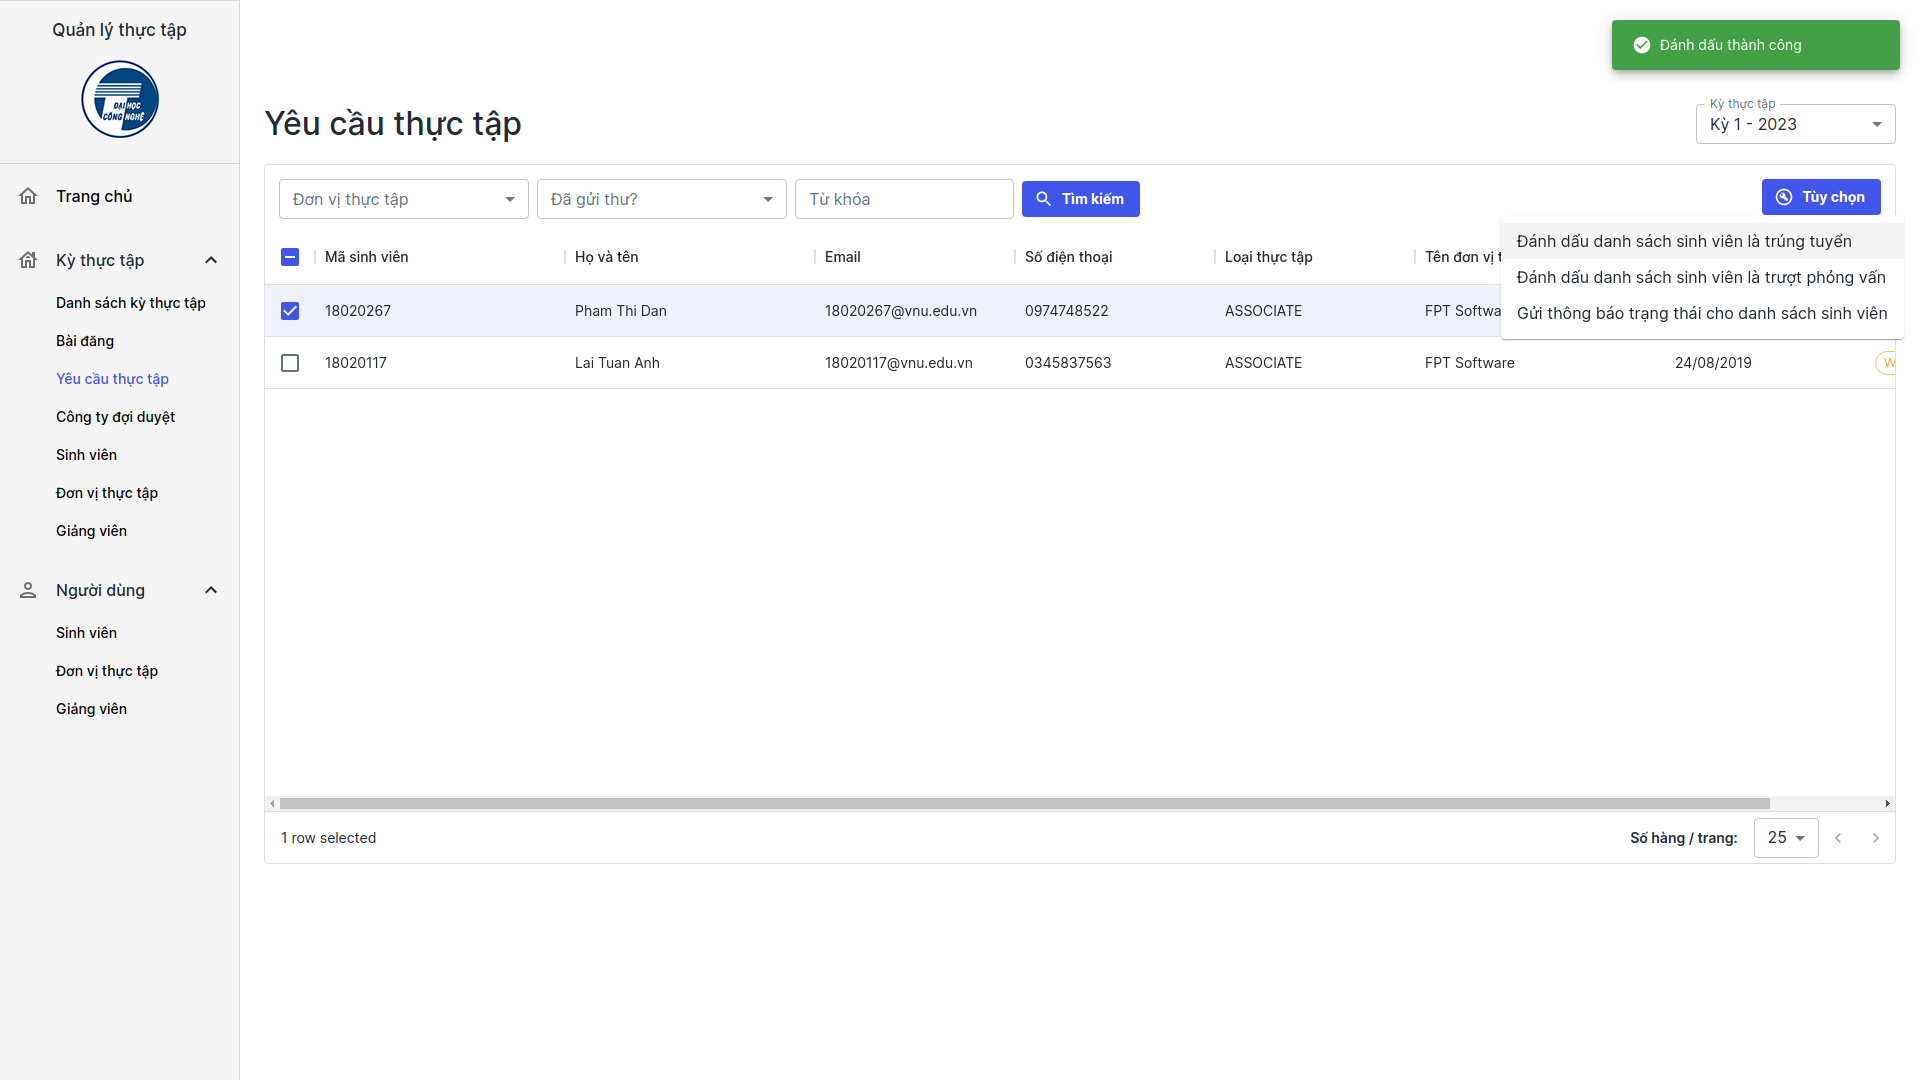
\includegraphics[width=\linewidth]{./images/image73.png}
	\caption{Luồng \emph{Quản trị viên Khoa chấp nhận / từ chối yêu cầu thực tập}: chọn danh sách sinh viên và chọn Chấp nhận / Từ chối}
	\label{fig:org_admin_select_requests}
\end{figure}

\paragraph*{Quản trị viên tải xuống danh sách sinh viên đã chốt đơn vị thực tập}

\begin{itemize}
	\item Hình \ref{fig:org_admin_access_list_intern_students}: Quản trị viên truy cập danh sách sinh viên trong kỳ thực tập. 
	\item Hình \ref{fig:org_admin_filter_students}: Quản trị viên lọc ra danh sách Sinh viên đã chốt đơn vị thực tập và chọn tùy chọn Xuất ra danh sách sinh viên.
\end{itemize}

\begin{figure}[]
	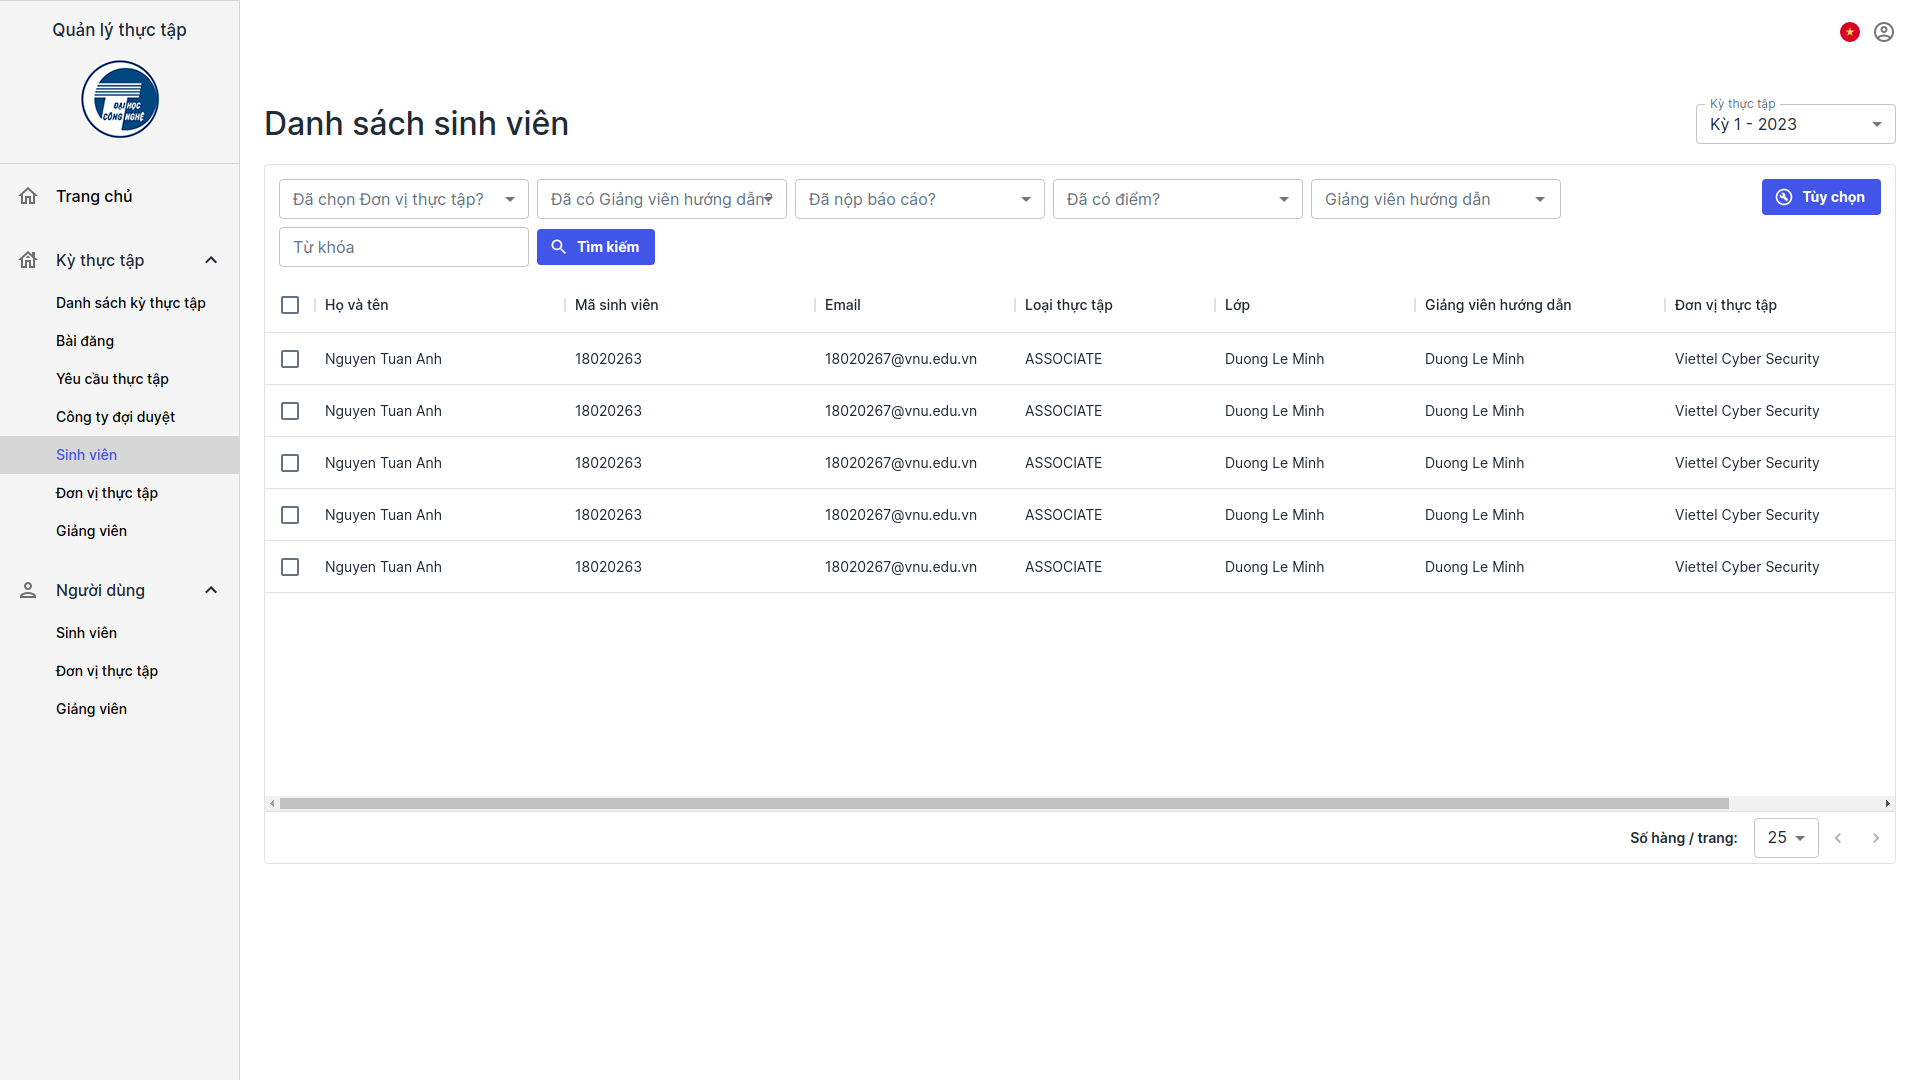
\includegraphics[width=\linewidth]{./images/image75.png}
	\caption{Luồng \emph{Quản trị viên tải xuống danh sách sinh viên đã chốt đơn vị thực tập}: truy cập danh sách sinh viên trong kỳ thực tập}
	\label{fig:org_admin_access_list_intern_students}
\end{figure}

\begin{figure}[]
	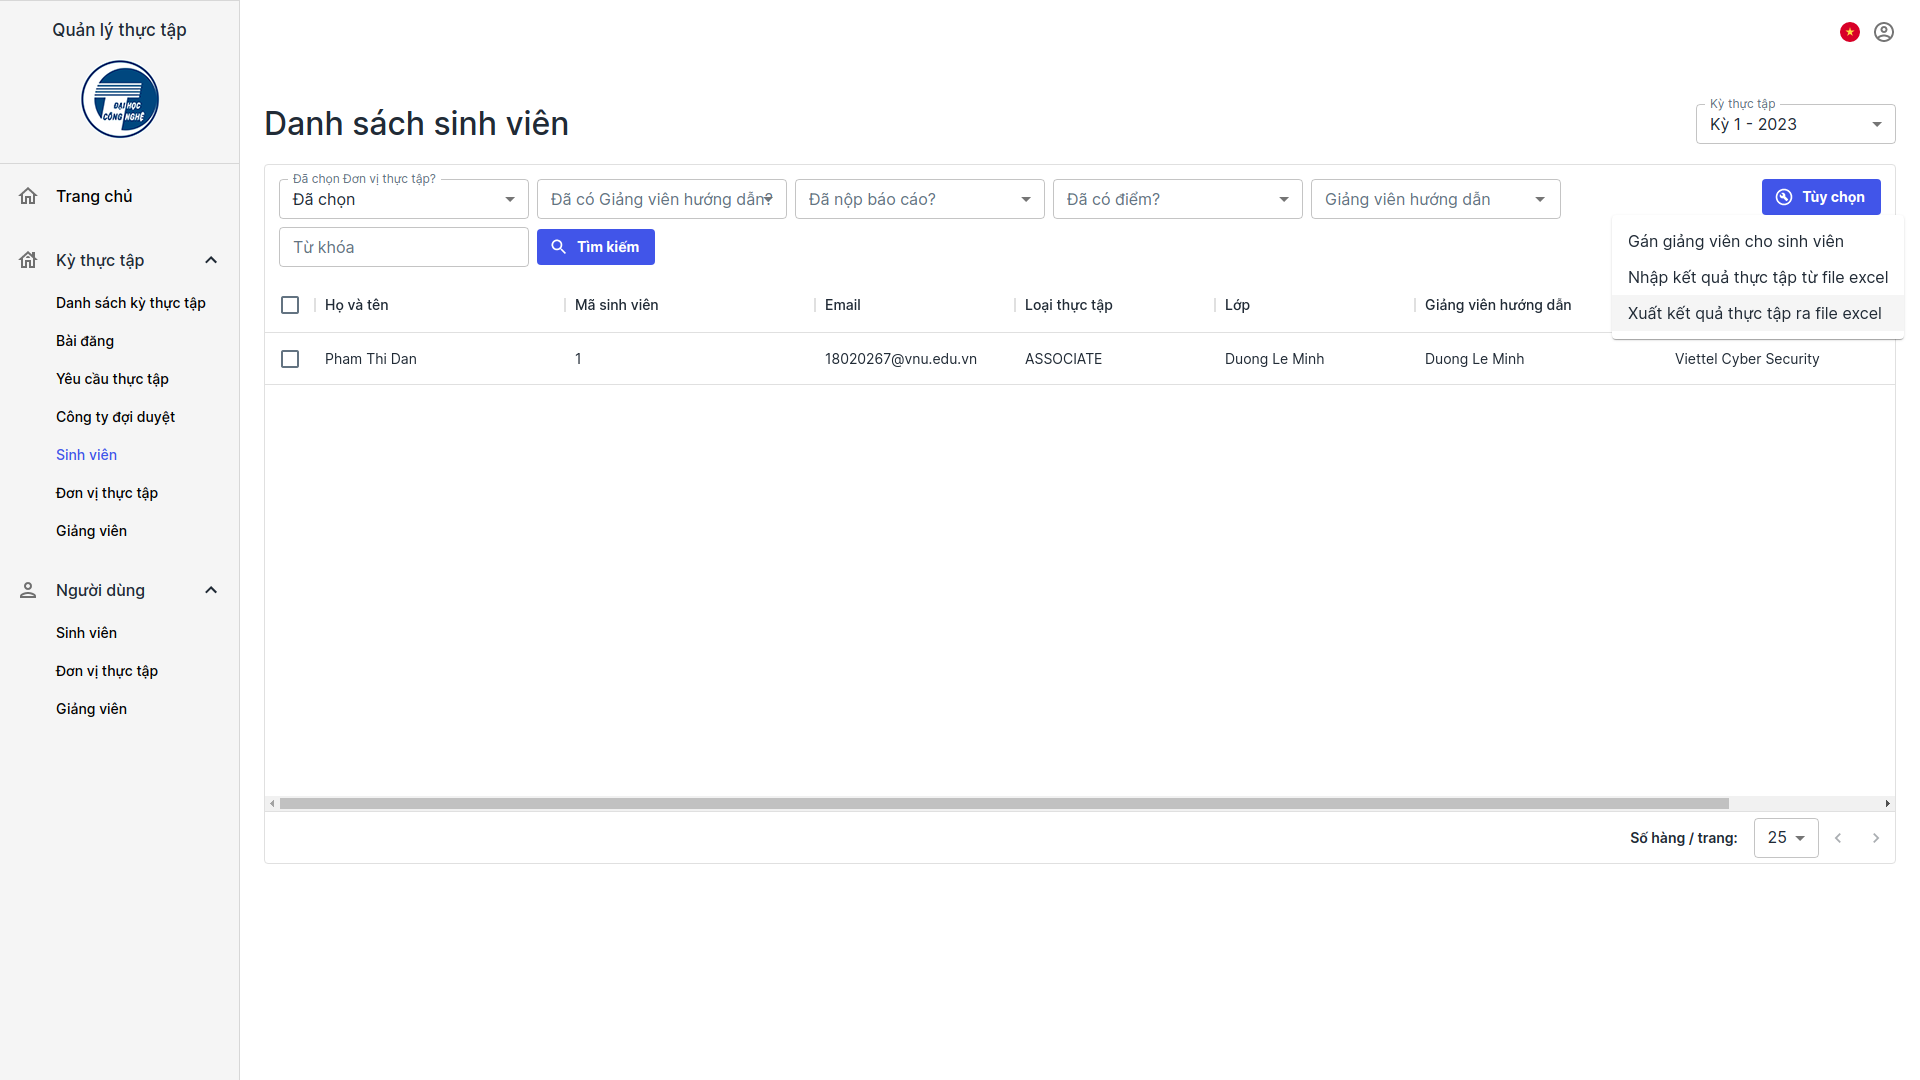
\includegraphics[width=\linewidth]{./images/image74.png}
	\caption{Luồng \emph{Quản trị viên tải xuống danh sách sinh viên đã chốt đơn vị thực tập}: lọc ra danh sách Sinh viên đã chốt đơn vị thực tập và chọn tùy chọn Xuất ra danh sách}
	\label{fig:org_admin_filter_students}
\end{figure}

\paragraph*{Quản trị viên Khoa gán giảng viên cho sinh viên}

\begin{itemize}
	\item Hình \ref{fig:org_admin_access_list_intern_students_1}: Quản trị viên khoa truy cập trang Danh sách sinh viên trong Kỳ thực tập. 
	\item Hình \ref{fig:org_admin_select_students}: Quản trị viên Khoa chọn danh sách sinh viên cần gán giảng viên và chọn tùy chọn Gán giảng viên.
	\item Hình \ref{fig:org_admin_select_lecturer}: Quản trị viên Khoa thực hiện chọn giảng viên để gán cho danh sách sinh viên.
	\item Hình \ref{fig:org_admin_assign_success}: Gán giảng viên thành công.
\end{itemize}

\begin{figure}[]
	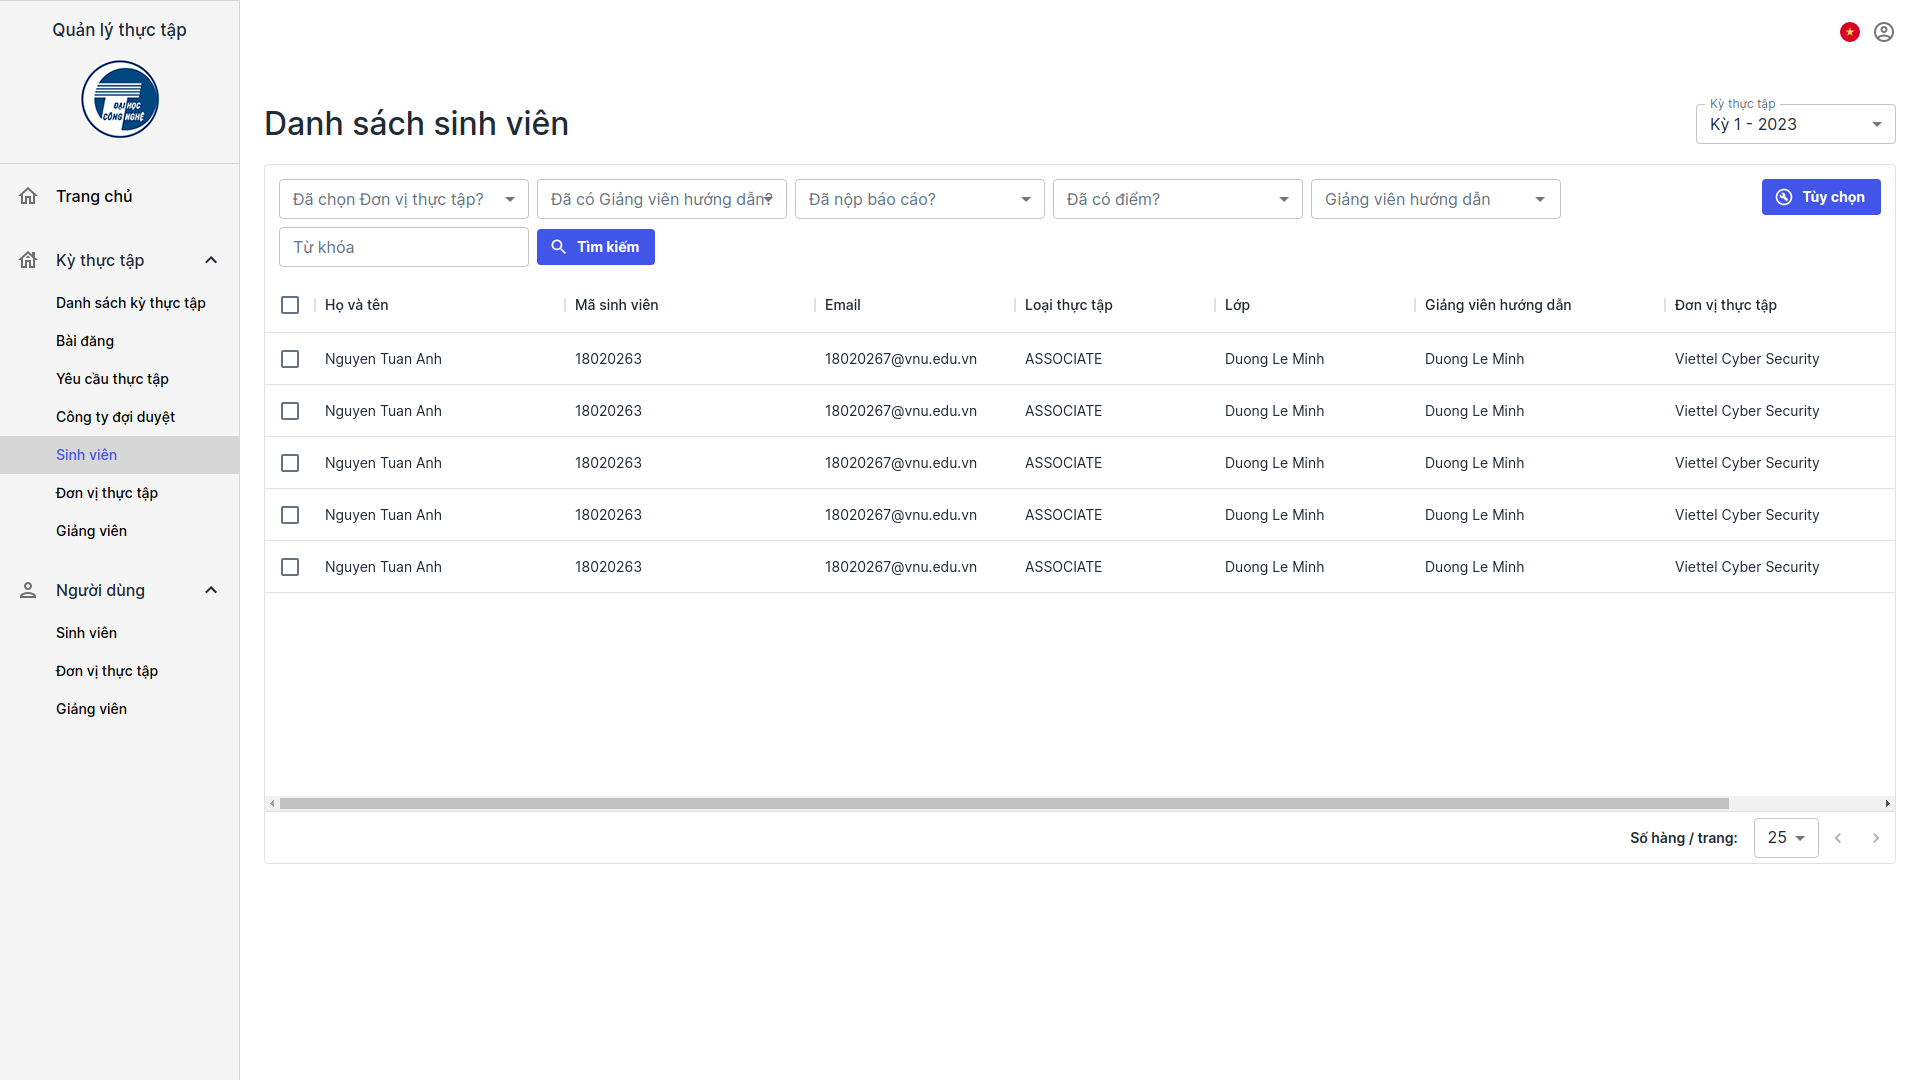
\includegraphics[width=\linewidth]{./images/image75.png}
	\caption{Luồng \emph{Quản trị viên Khoa gán giảng viên cho sinh viên}: truy cập danh sách sinh viên trong kỳ thực tập}
	\label{fig:org_admin_access_list_intern_students_1}
\end{figure}

\begin{figure}[]
	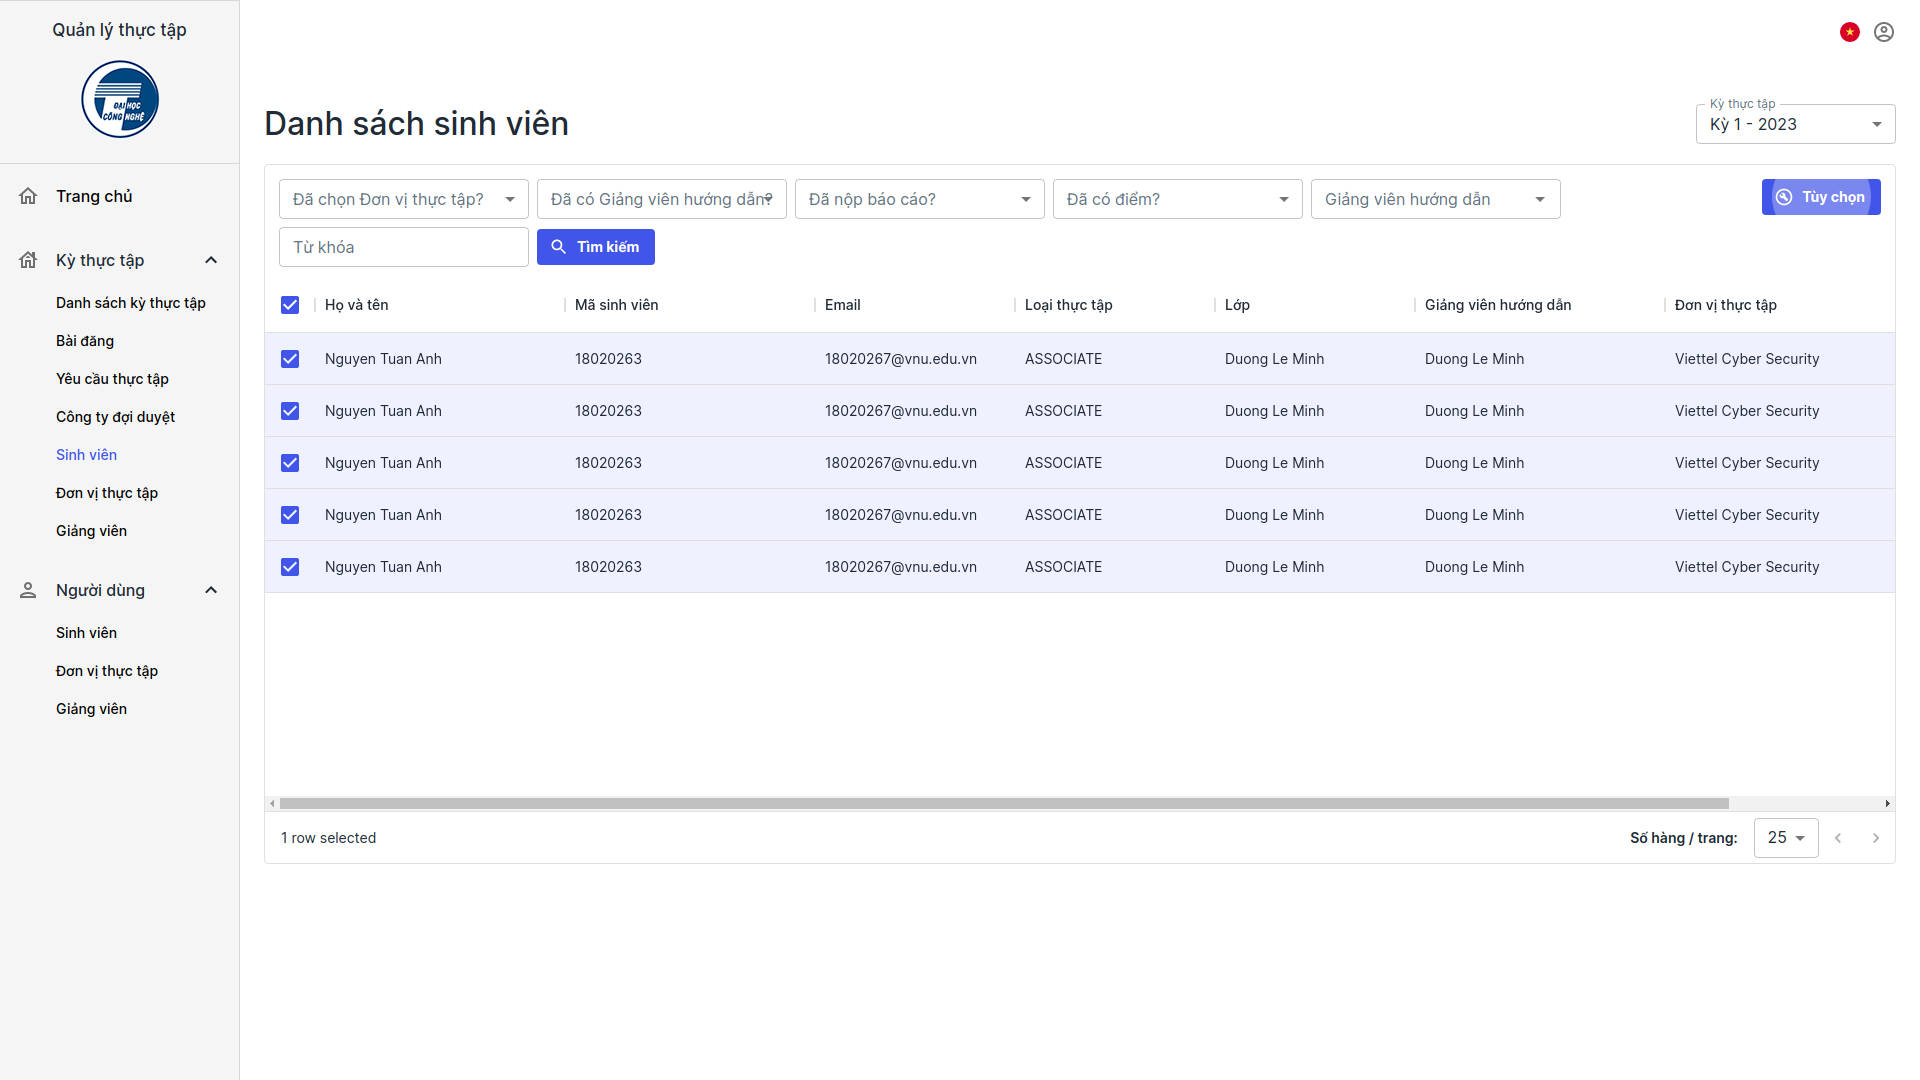
\includegraphics[width=\linewidth]{./images/image76.png}
	\caption{Luồng \emph{Quản trị viên Khoa gán giảng viên cho sinh viên}: chọn danh sách sinh viên cần gán}
	\label{fig:org_admin_select_students}
\end{figure}

\begin{figure}[]
	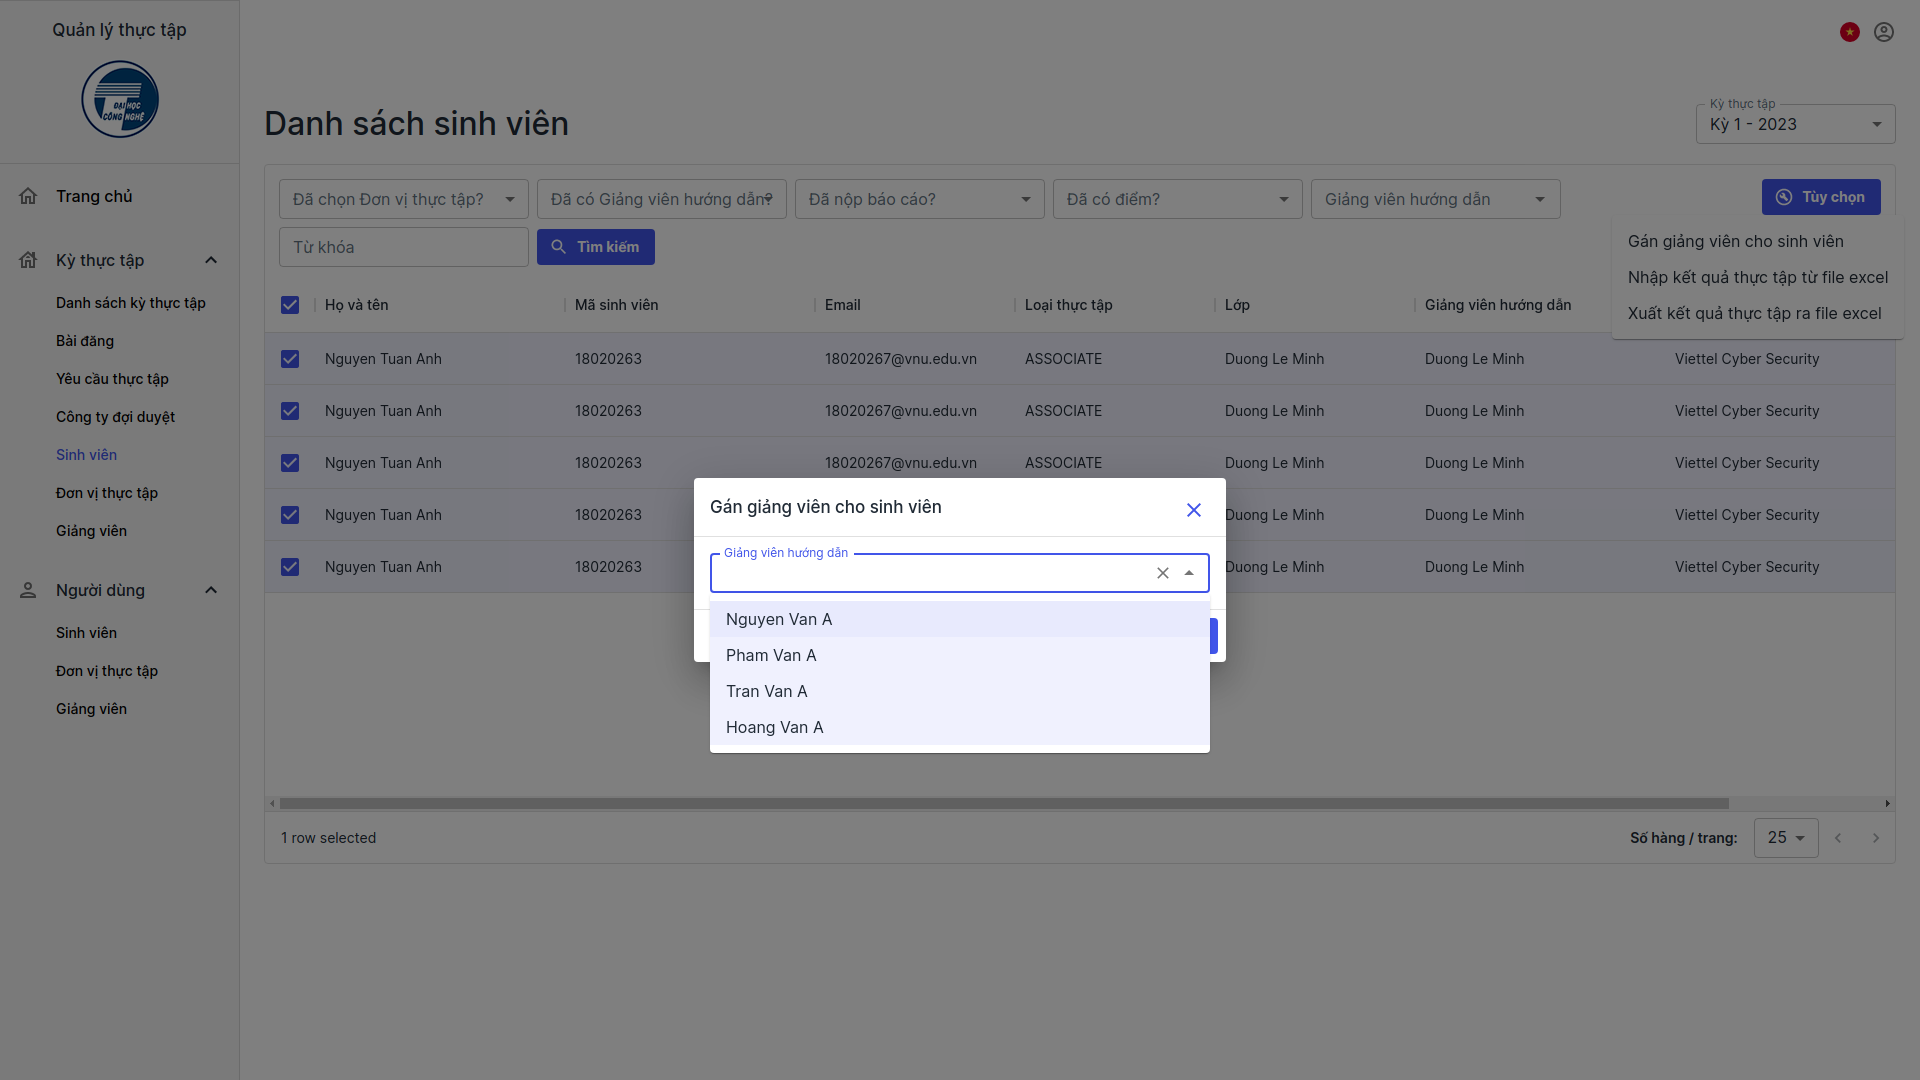
\includegraphics[width=\linewidth]{./images/image77.png}
	\caption{Luồng \emph{Quản trị viên Khoa gán giảng viên cho sinh viên}: chọn giảng viên}
	\label{fig:org_admin_select_lecturer}
\end{figure}

\begin{figure}[]
	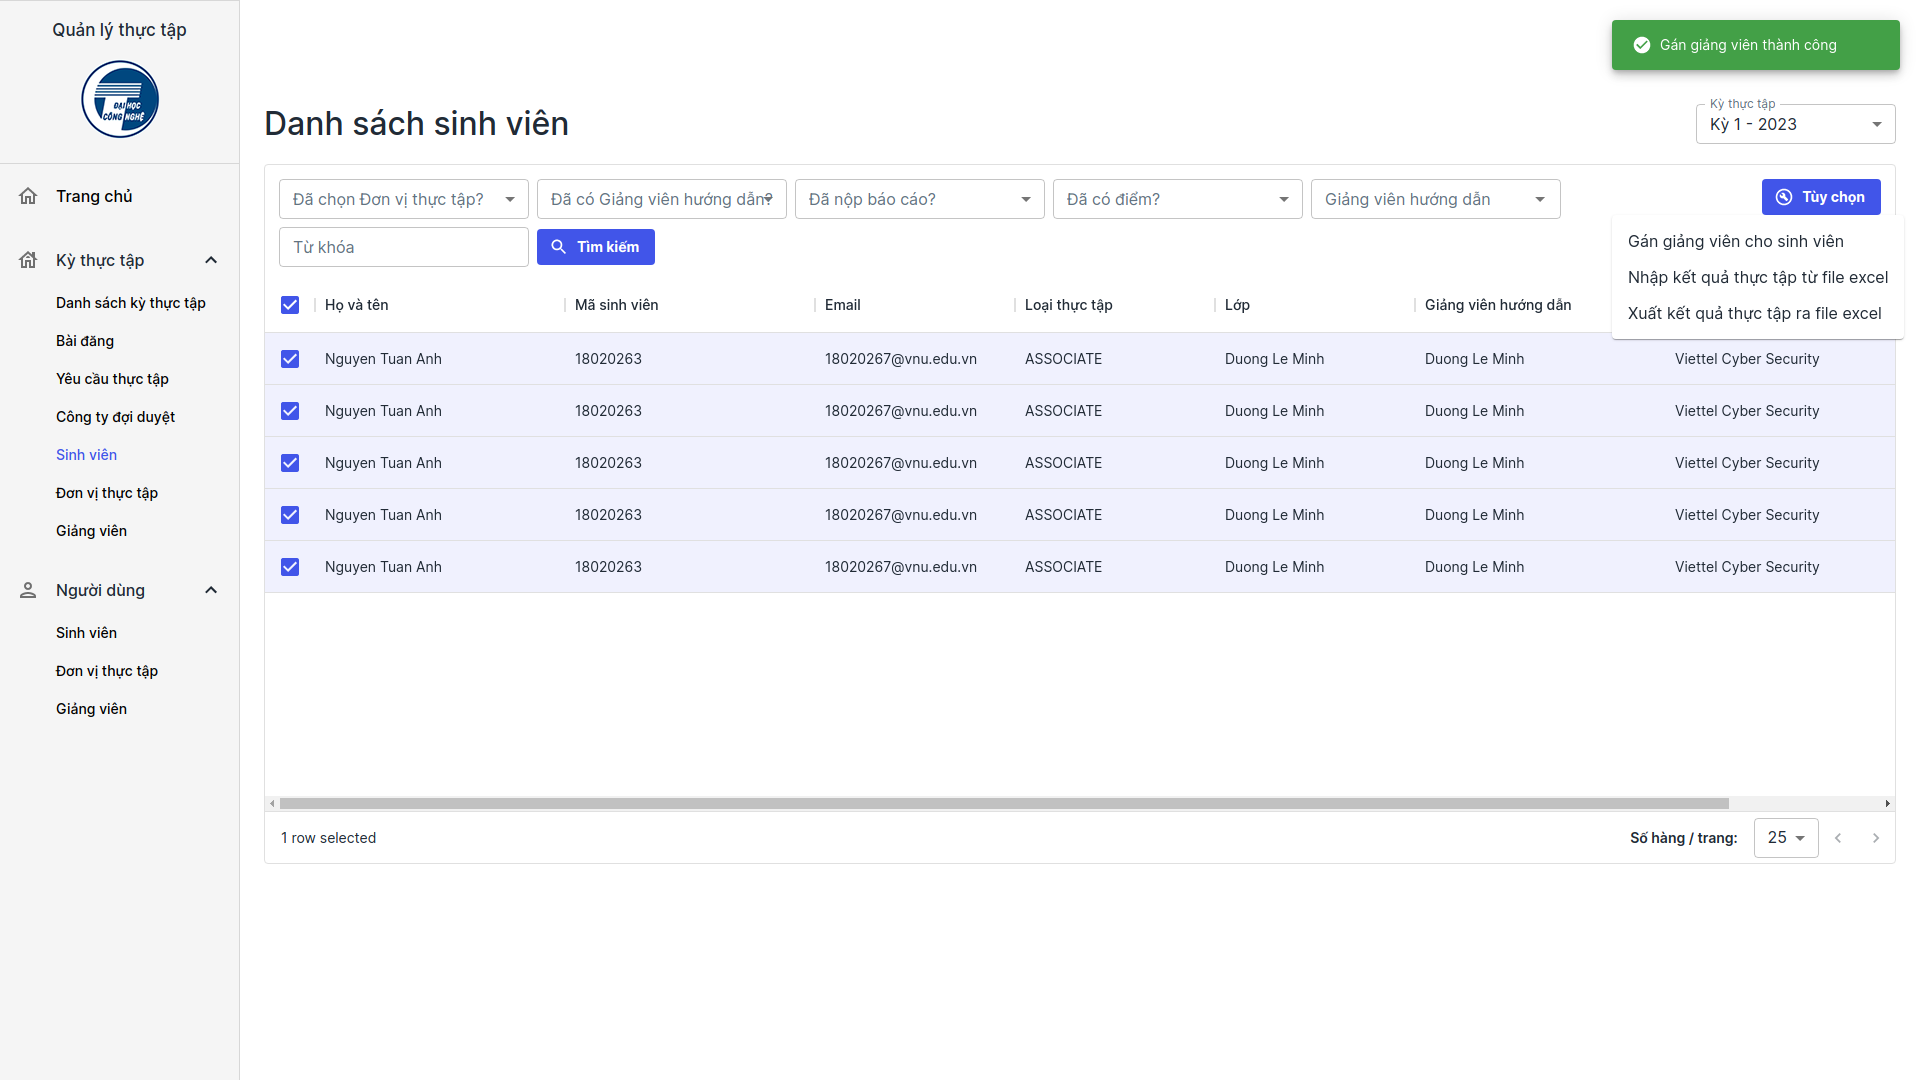
\includegraphics[width=\linewidth]{./images/image78.png}
	\caption{Luồng \emph{Quản trị viên Khoa gán giảng viên cho sinh viên}: gán giảng viên thành công}
	\label{fig:org_admin_assign_success}
\end{figure}

\paragraph*{Quản trị viên Khoa Chấp nhận / Từ chối công ty}

\begin{itemize}
	\item Hình \ref{fig:org_admin_access_list_intern_partners}: Quản trị viên truy cập danh sách Đơn vị thực tập trong kỳ thực tập và lọc ra danh sách các công ty đang ở trạng thái Pending. 
	\item Hình \ref{fig:org_admin_select_partners}: Quản trị viên chọn danh sách công ty và chọn tùy chọn Chấp nhận / Từ chối công ty.
\end{itemize}

\begin{figure}[]
	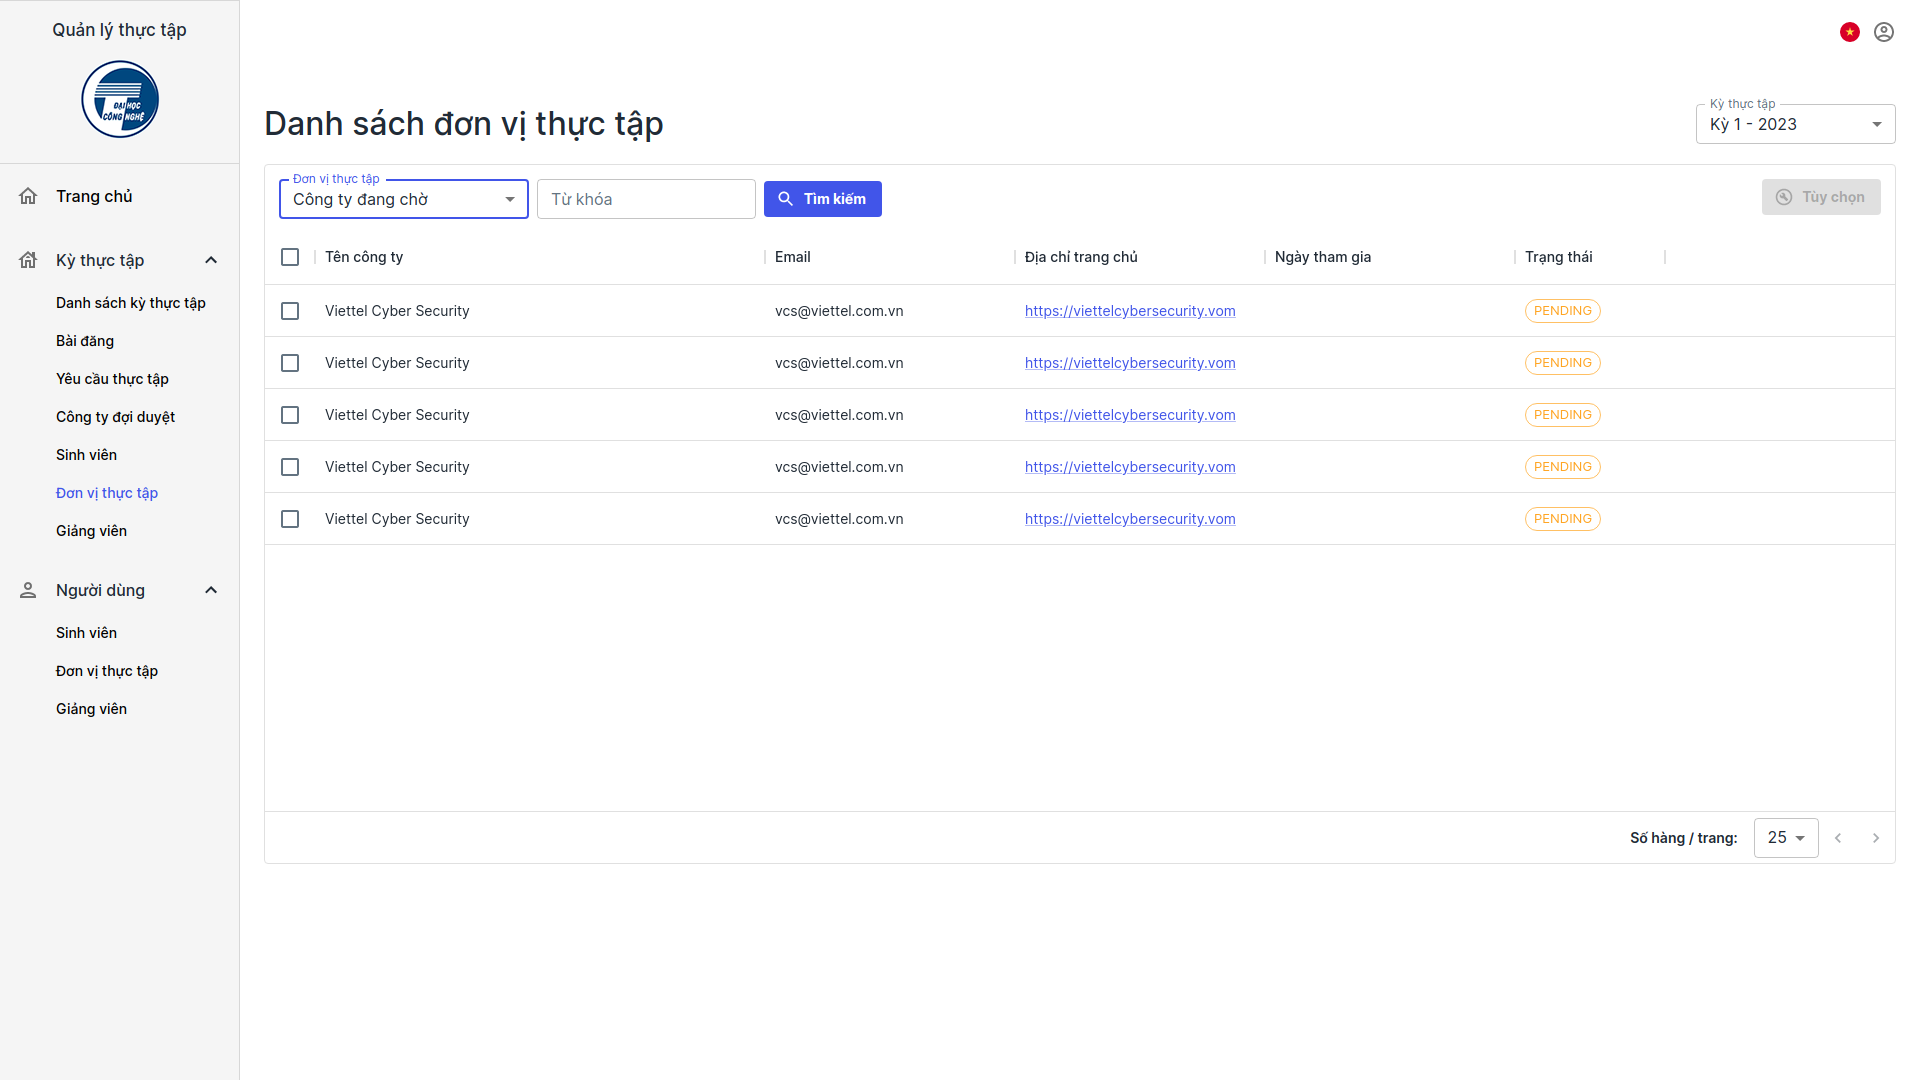
\includegraphics[width=\linewidth]{./images/image79.png}
	\caption{Luồng \emph{Quản trị viên Khoa Chấp nhận / Từ chối công ty}: truy cập danh sách đơn vị thực tập và lọc ra danh sách các công ty đang ở trạng thái Pending}
	\label{fig:org_admin_access_list_intern_partners}
\end{figure}

\begin{figure}[]
	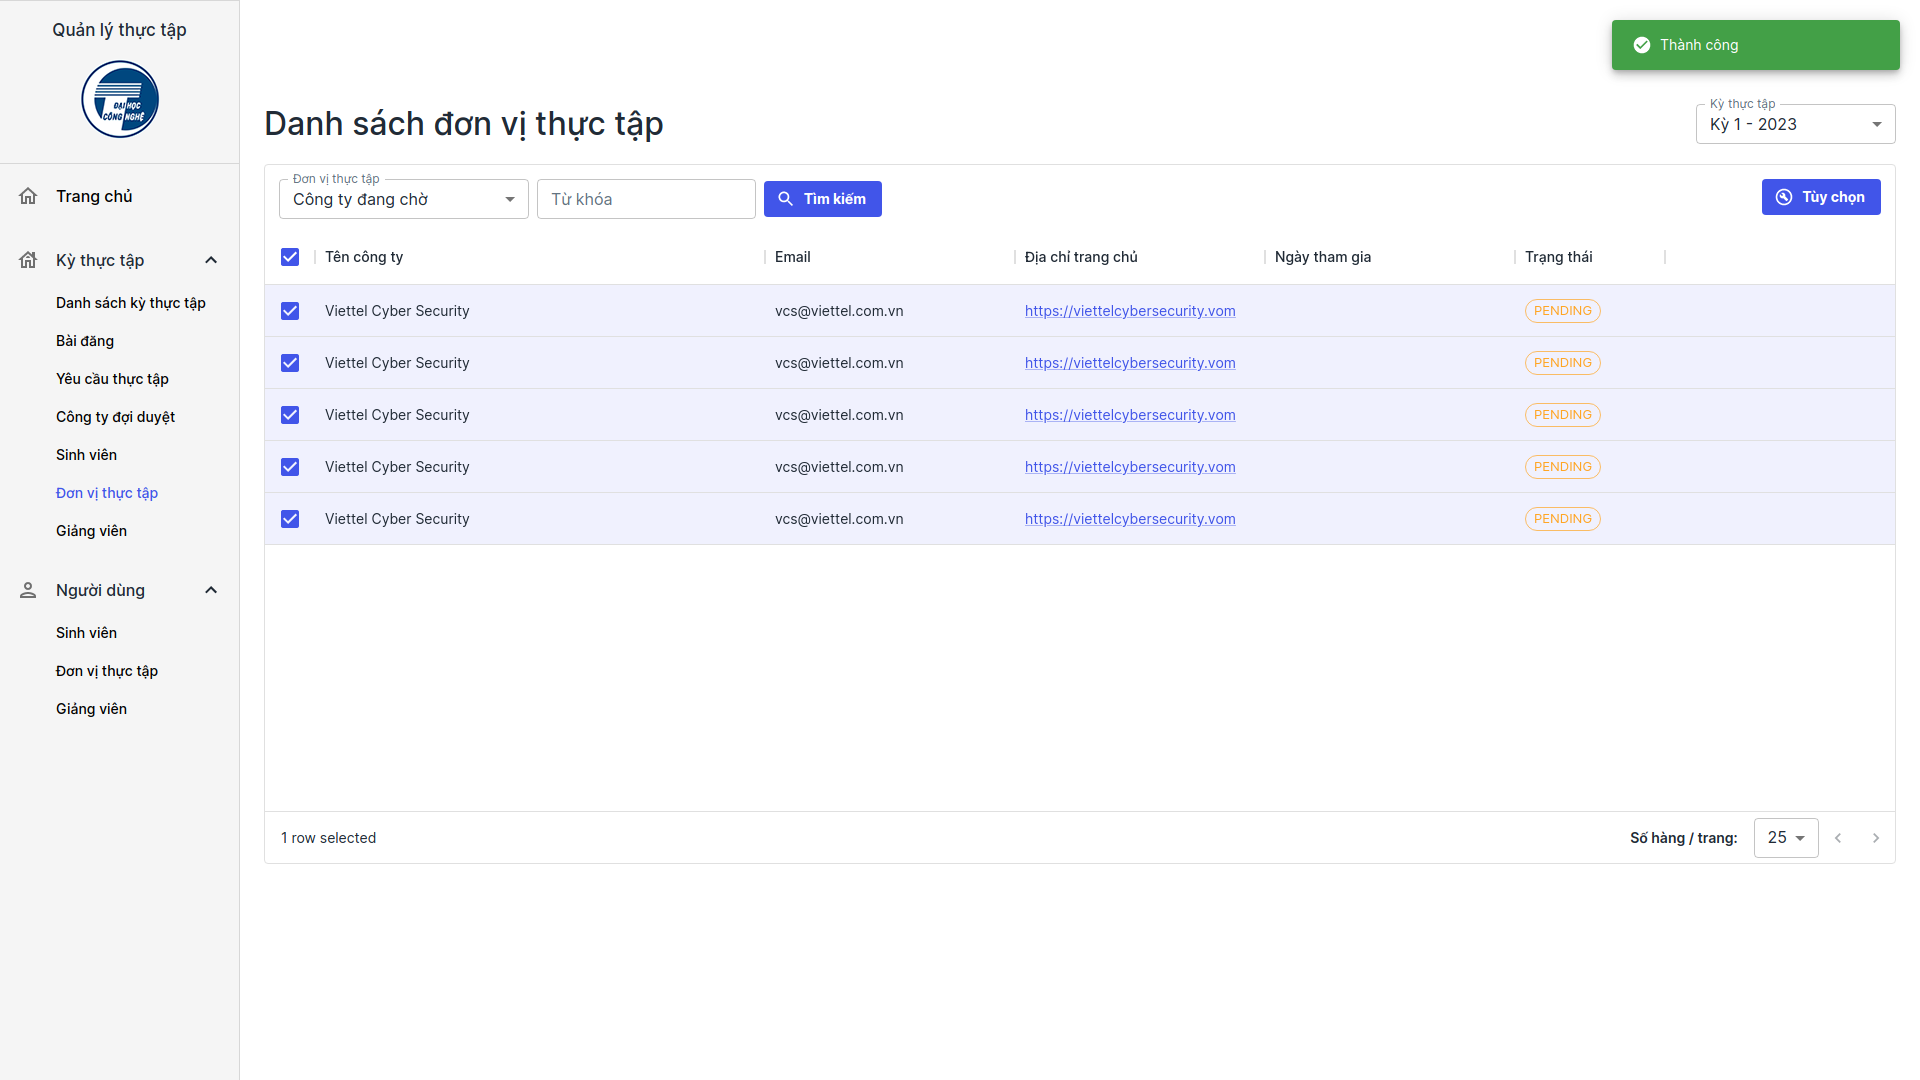
\includegraphics[width=\linewidth]{./images/image80.png}
	\caption{Luồng \emph{Quản trị viên Khoa Chấp nhận / Từ chối công ty}: chọn danh sách đơn vị thực tập và chọn tùy chọn Chấp nhận / Từ chối công ty}
	\label{fig:org_admin_select_partners}
\end{figure}

\subsection{Luồng sử dụng của quản trị viên hệ thống}

\paragraph*{Quản trị viên tạo Khoa mới}

\begin{itemize}
	\item Hình \ref{fig:admin_access_list_orgs}: Quản trị viên truy cập danh sách Khoa. 
	\item Hình \ref{fig:admin_add_org}: Quản trị viên chọn Thêm Khoa mới và thực hiện tạo mới.
	\item Hình \ref{fig:admin_add_org_success}: Tạo mới thành công.
\end{itemize}

\begin{figure}[]
	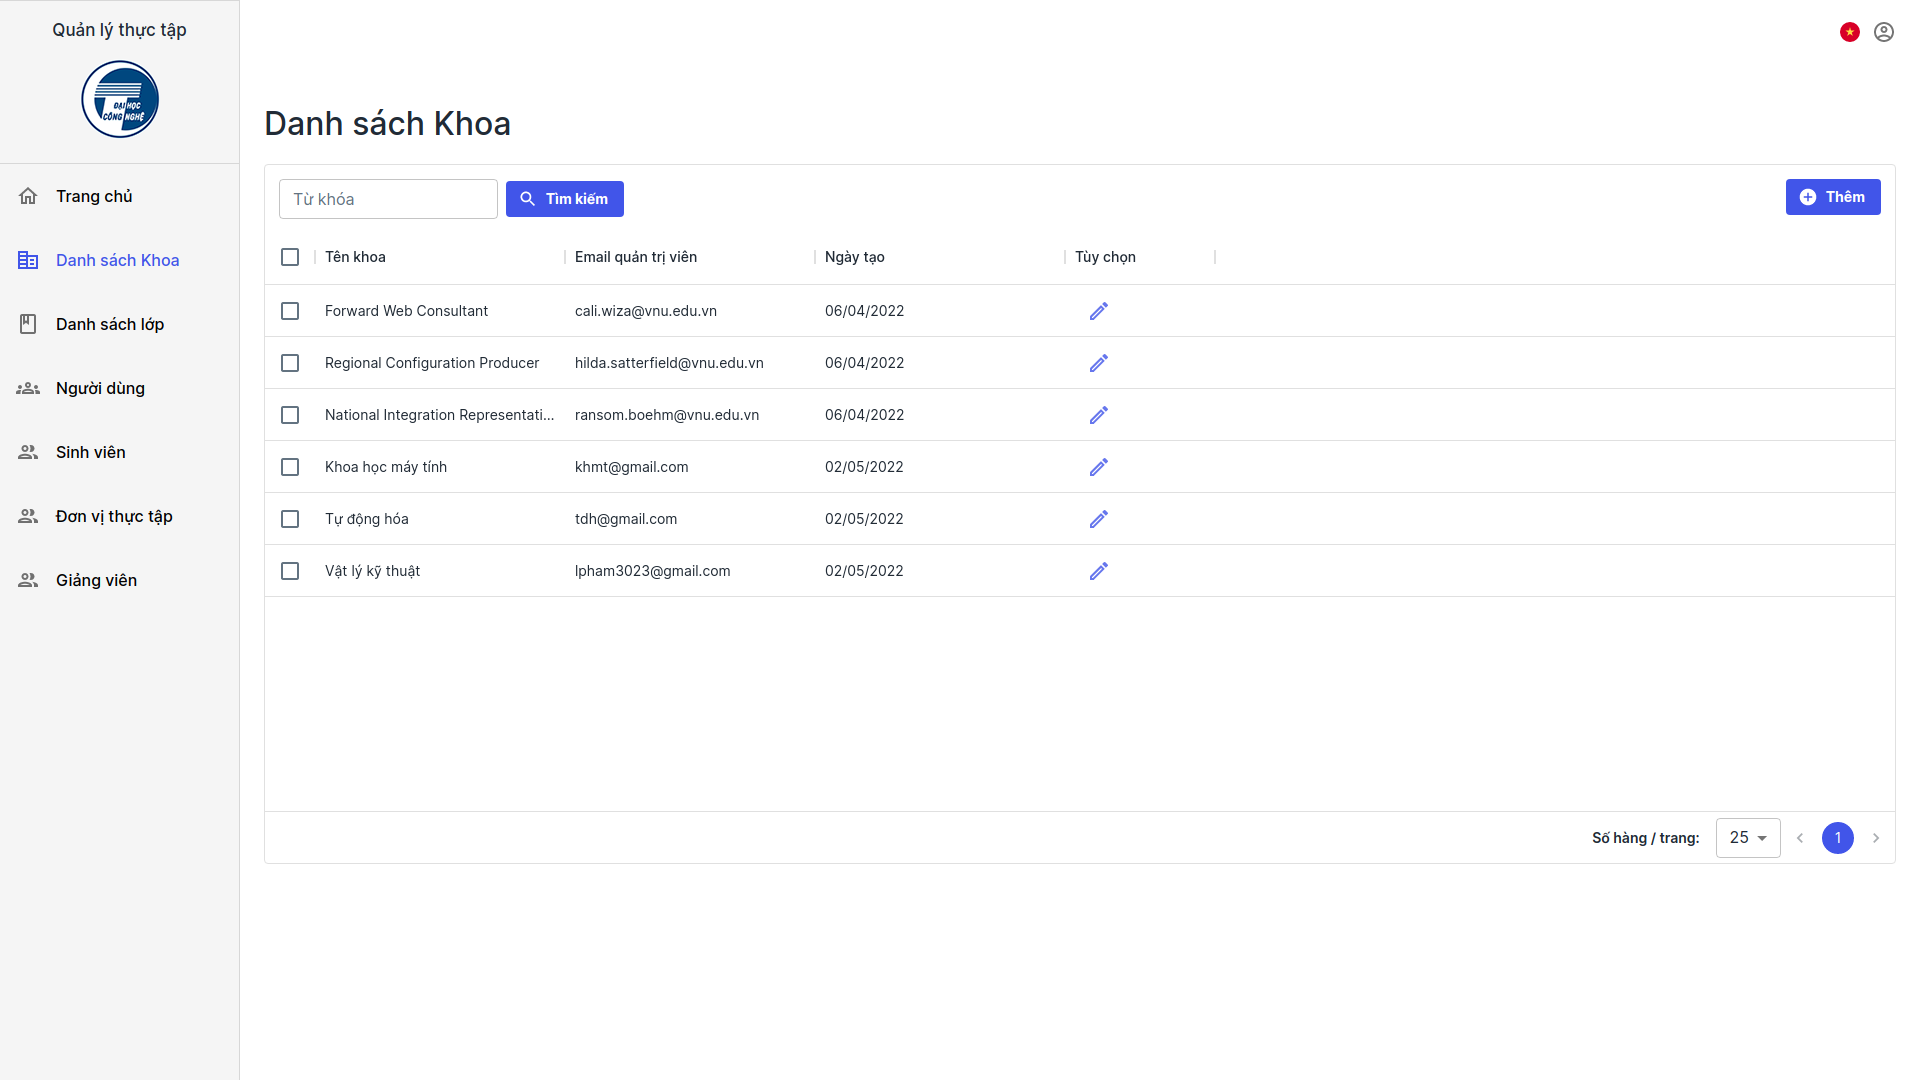
\includegraphics[width=\linewidth]{./images/image56.png}
	\caption{Luồng \emph{Quản trị viên tạo Khoa mới}: truy cập danh sách Khoa}
	\label{fig:admin_access_list_orgs}
\end{figure}

\begin{figure}[]
	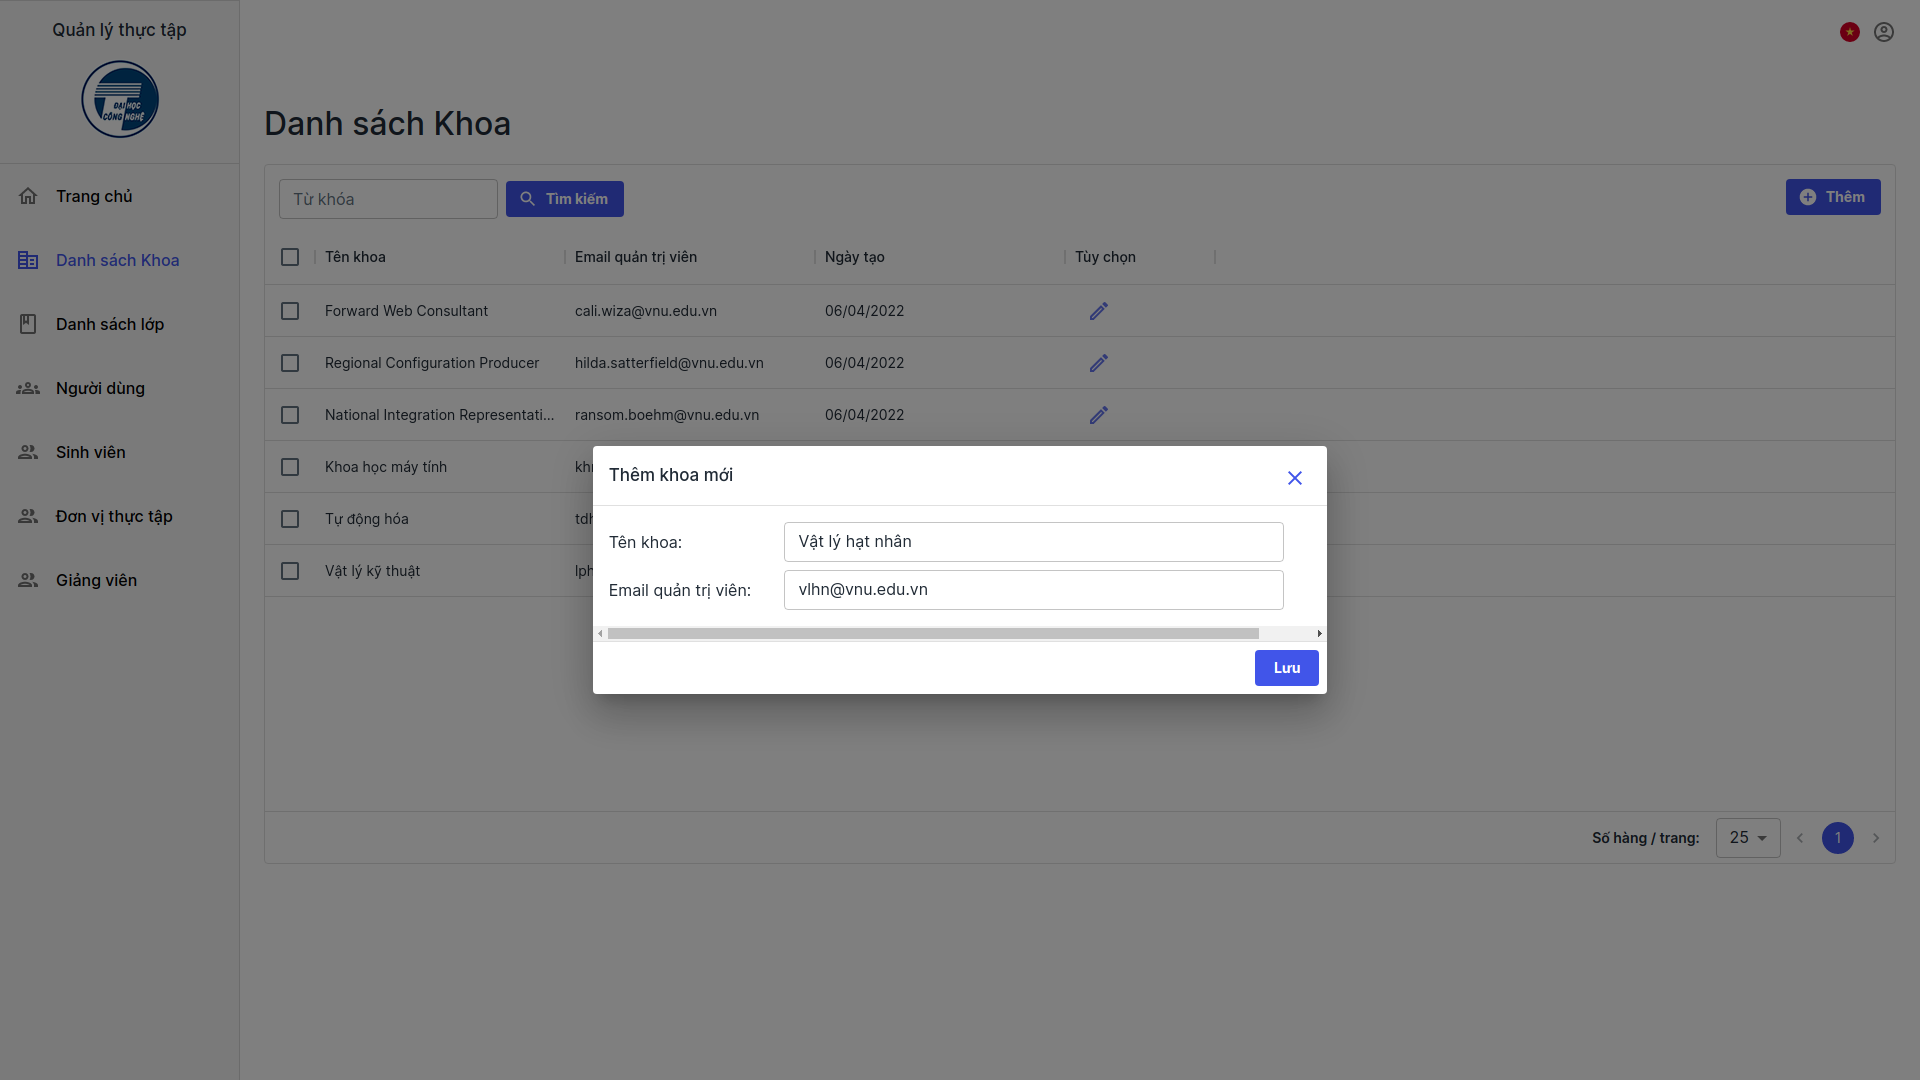
\includegraphics[width=\linewidth]{./images/image57.png}
	\caption{Luồng \emph{Quản trị viên tạo Khoa mới}: chọn Thêm Khoa mới và thực hiện tạo mới}
	\label{fig:admin_add_org}
\end{figure}

\begin{figure}[]
	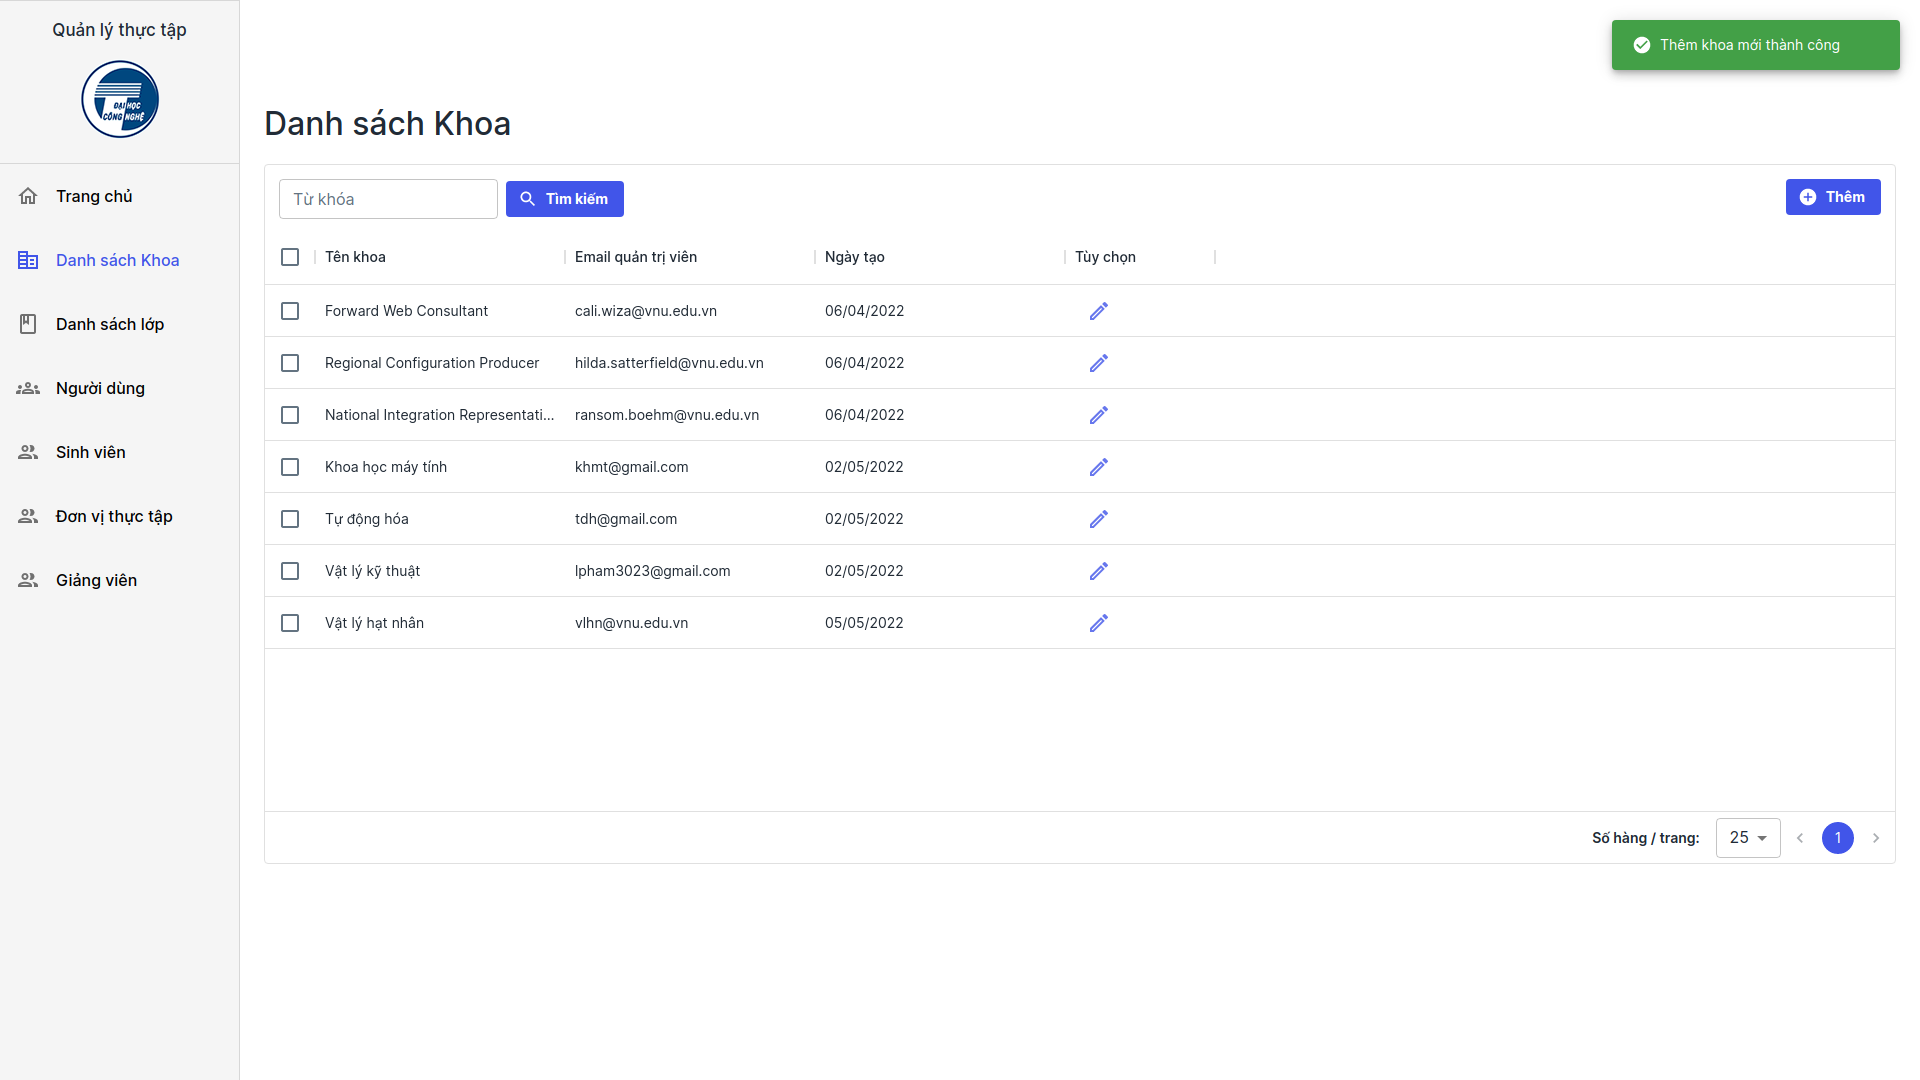
\includegraphics[width=\linewidth]{./images/image58.png}
	\caption{Luồng \emph{Quản trị viên tạo Khoa mới}: Tạo mới thành công}
	\label{fig:admin_add_org_success}
\end{figure}

\paragraph*{Quản trị viên tạo Lớp mới}

\begin{itemize}
	\item Hình \ref{fig:admin_access_list_classes}: Quản trị viên truy cập danh sách lớp. 
	\item Hình \ref{fig:admin_add_class}: Quản trị viên chọn Thêm lớp và thực hiện tạo mới.
	\item Hình \ref{fig:admin_add_class_success}: Tạo mới thành công.
\end{itemize}

\begin{figure}[]
	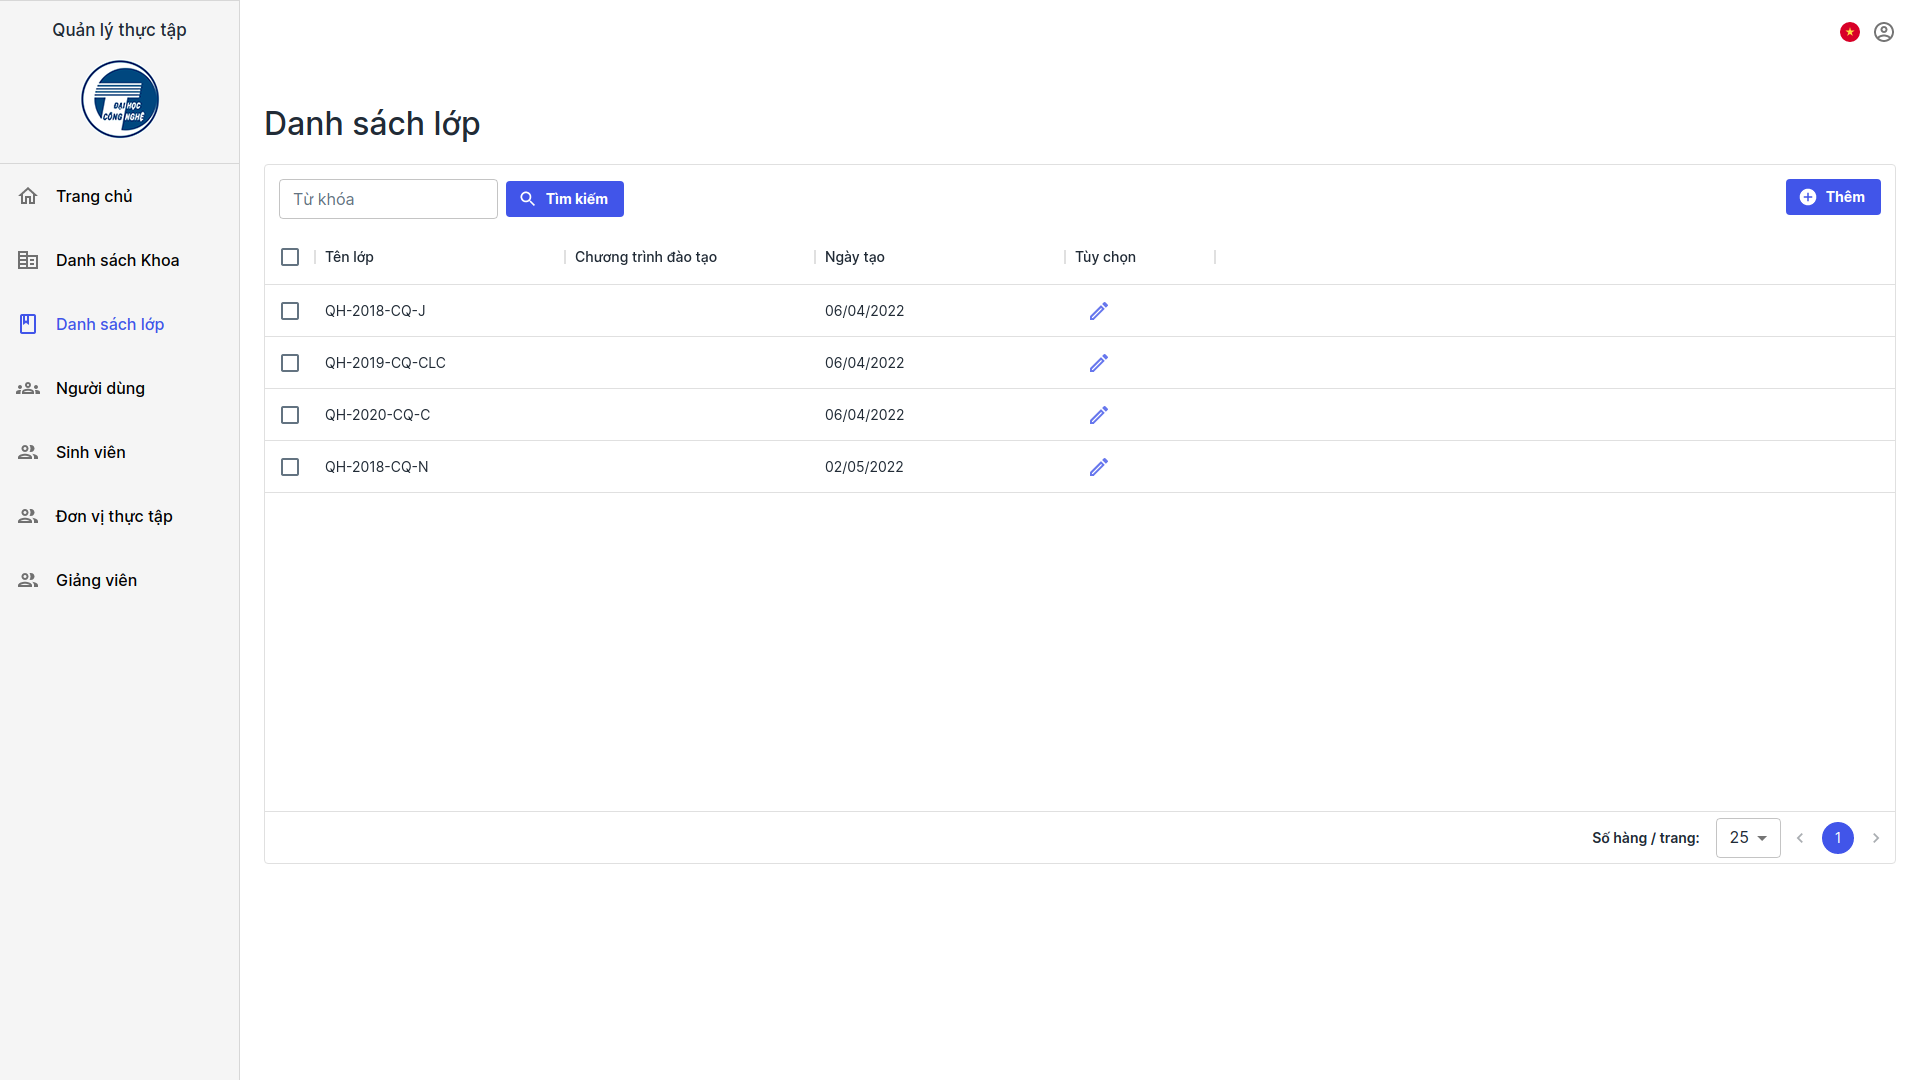
\includegraphics[width=\linewidth]{./images/image59.png}
	\caption{Luồng \emph{Quản trị viên tạo Lớp mới}: truy cập danh sách Lớp}
	\label{fig:admin_access_list_classes}
\end{figure}

\begin{figure}[]
	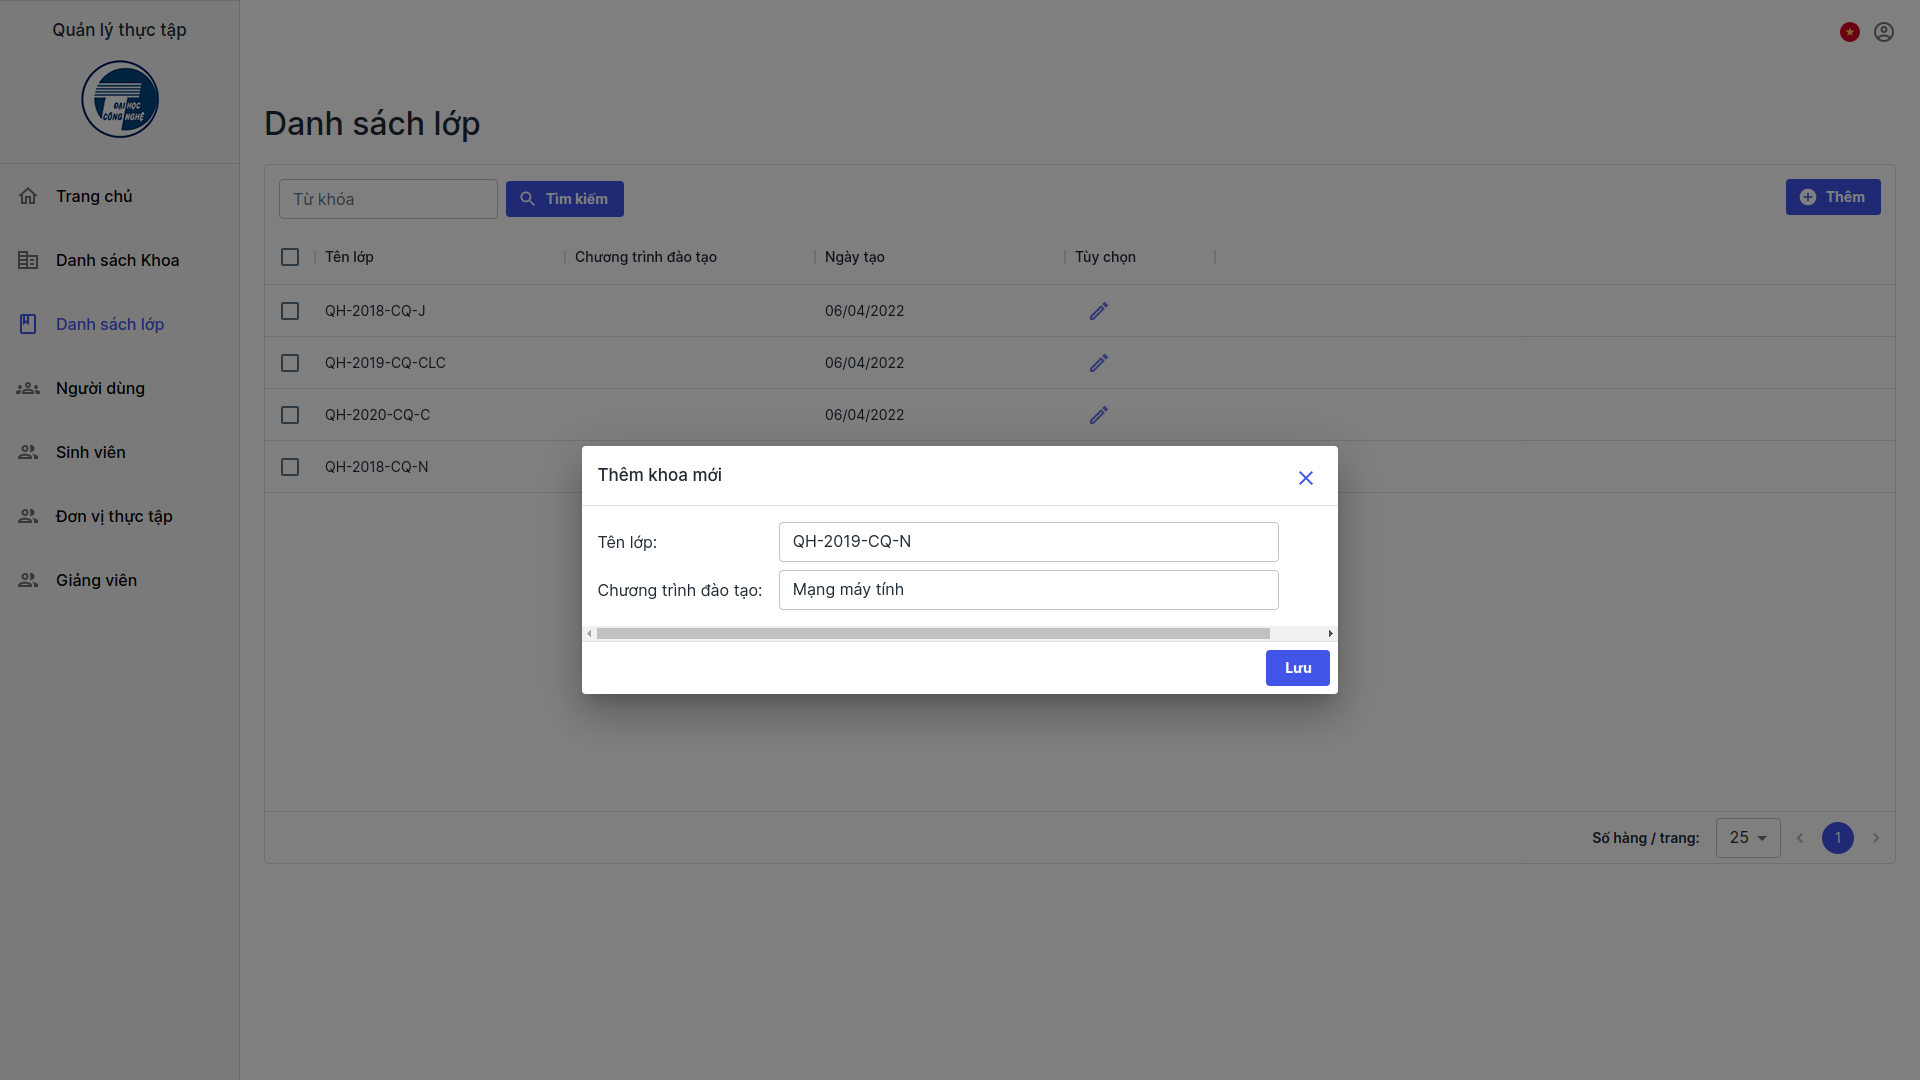
\includegraphics[width=\linewidth]{./images/image60.png}
	\caption{Luồng \emph{Quản trị viên tạo Lớp mới}: chọn Thêm Lớp mới và thực hiện tạo mới}
	\label{fig:admin_add_class}
\end{figure}

\begin{figure}[]
	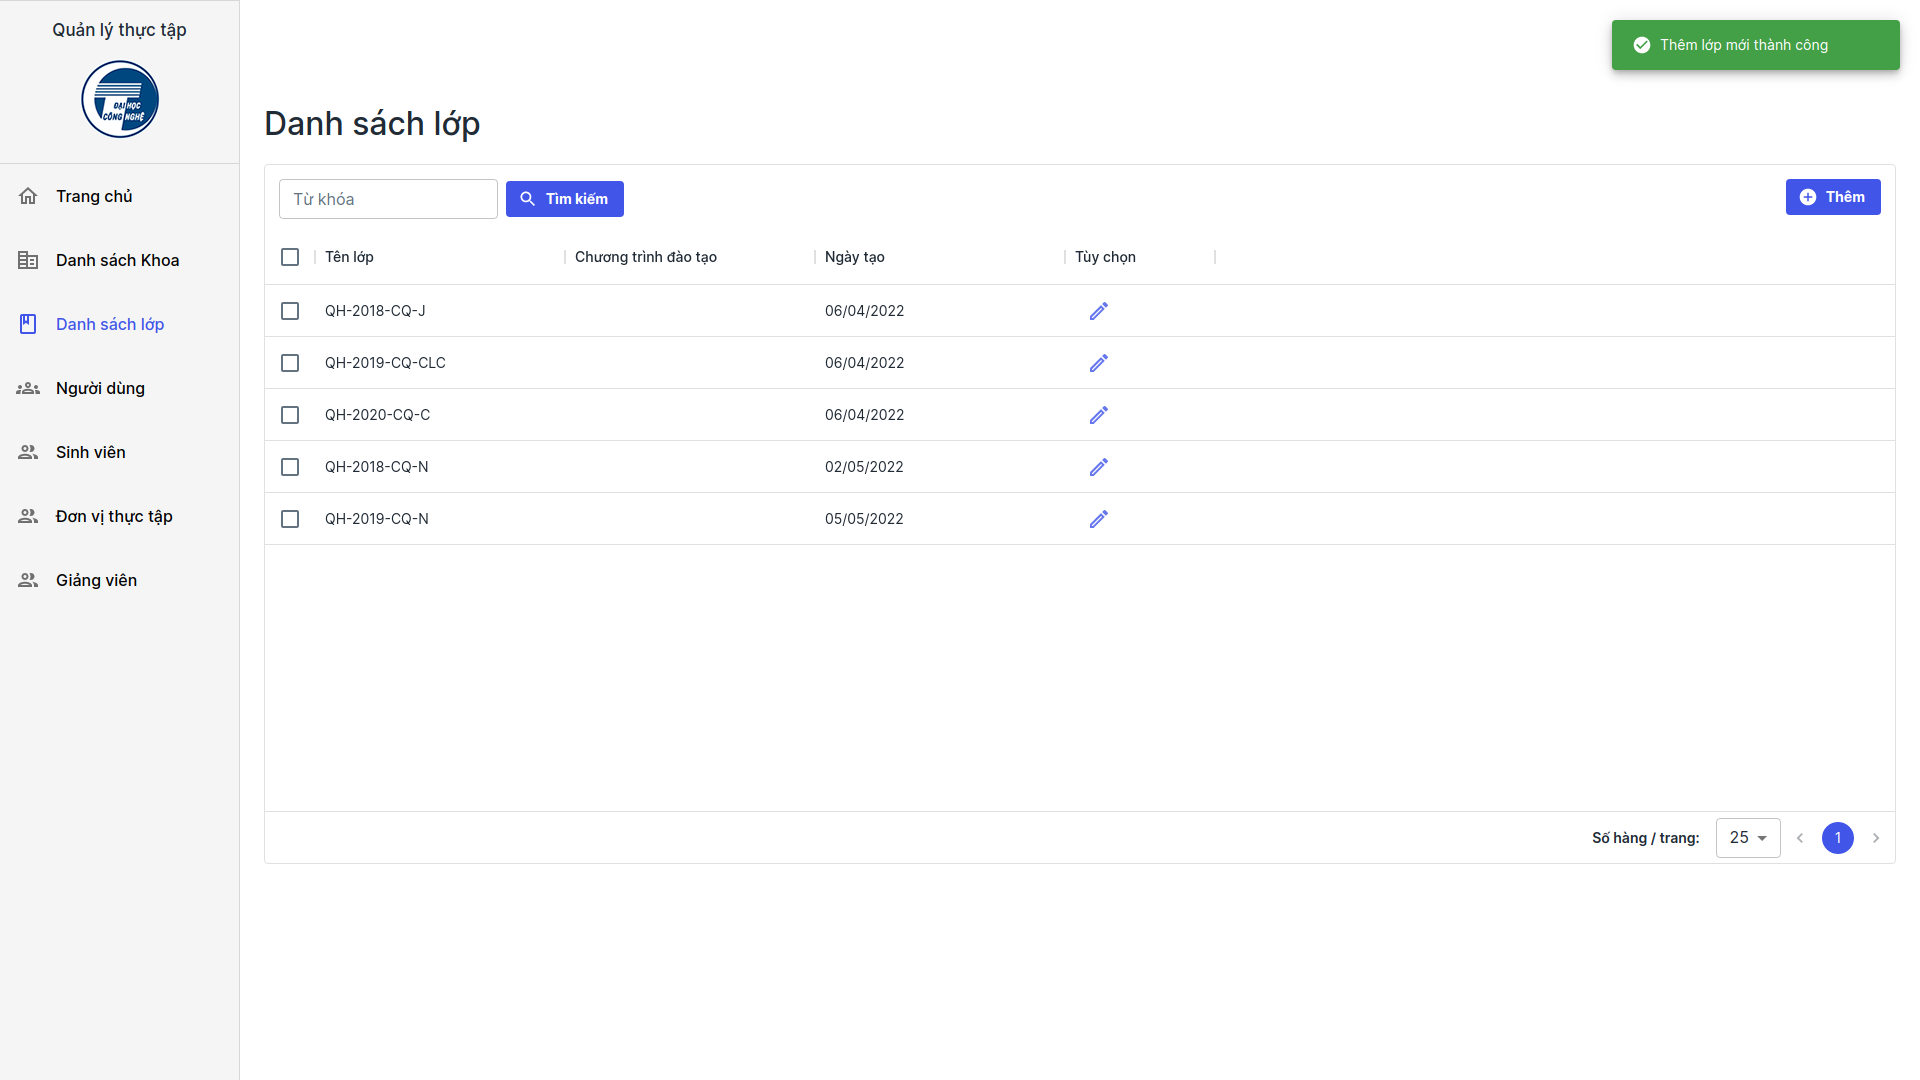
\includegraphics[width=\linewidth]{./images/image61.png}
	\caption{Luồng \emph{Quản trị viên tạo Lớp mới}: Tạo mới thành công}
	\label{fig:admin_add_class_success}
\end{figure}

\paragraph*{Quản trị viên nhập vào Danh sách sinh viên}

\begin{itemize}
	\item Hình \ref{fig:admin_access_list_students}: Quản trị viên truy cập danh sách sinh viên và mở tùy chọn. 
	\item Hình \ref{fig:choose_file}: Quản trị viên chọn Nhập danh sách sinh viên từ file excel và chọn tệp.
	\item Hình \ref{fig:upload_list}: Quản trị viên duyệt qua danh sách sau khi chọn tệp và tải lên danh sách.
\end{itemize}

\begin{figure}[]
	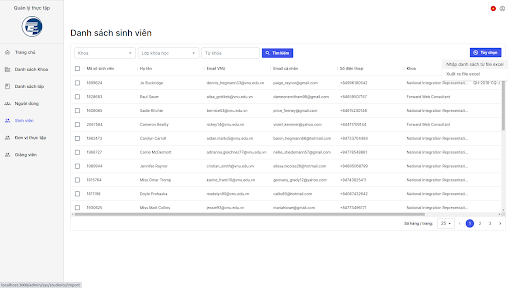
\includegraphics[width=\linewidth]{./images/image68.png}
	\caption{Luồng \emph{Quản trị viên nhập vào Danh sách sinh viên}: truy cập danh sách sinh viên và mở tùy chọn}
	\label{fig:admin_access_list_students}
\end{figure}

\begin{figure}[]
	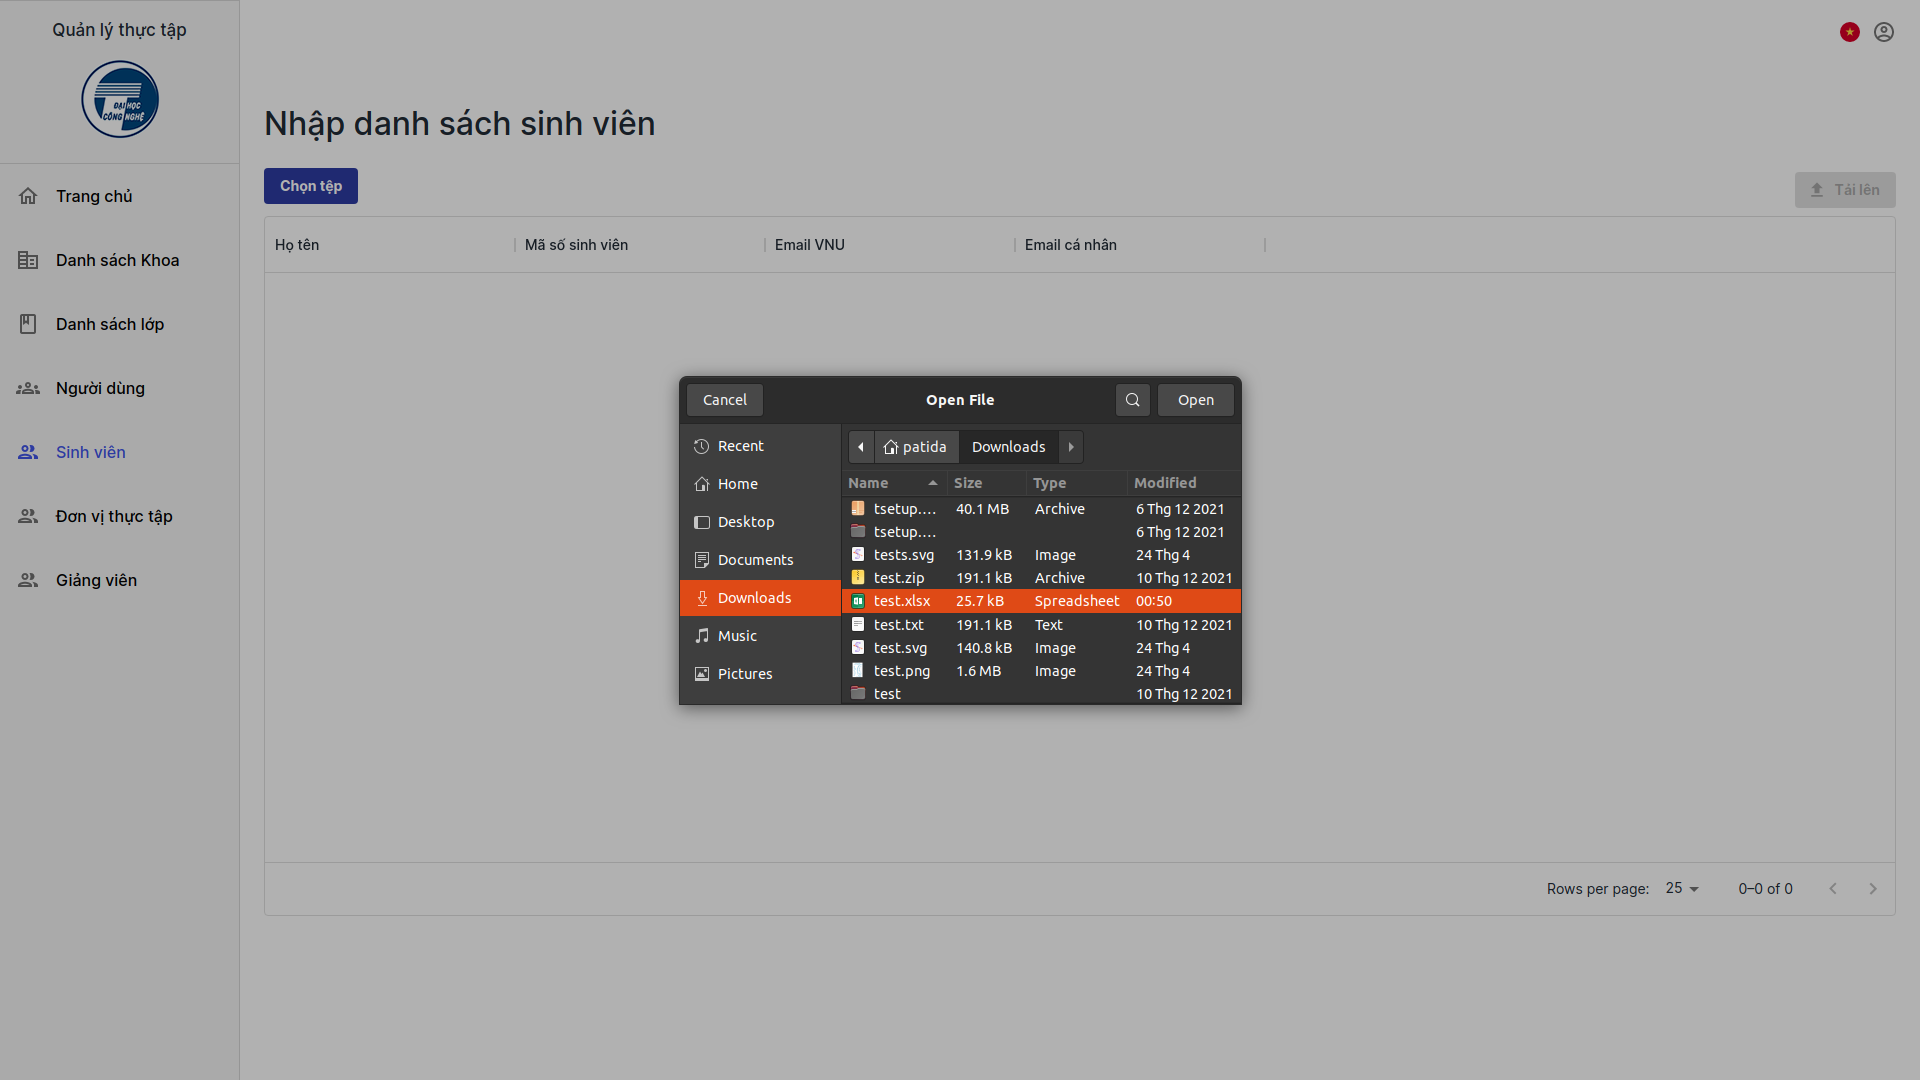
\includegraphics[width=\linewidth]{./images/image27.png}
	\caption{Luồng \emph{Quản trị viên nhập vào Danh sách sinh viên}: chọn Nhập danh sách sinh viên từ file excel và chọn tệp danh sách sinh viên}
	\label{fig:choose_file}
\end{figure}

\begin{figure}[]
	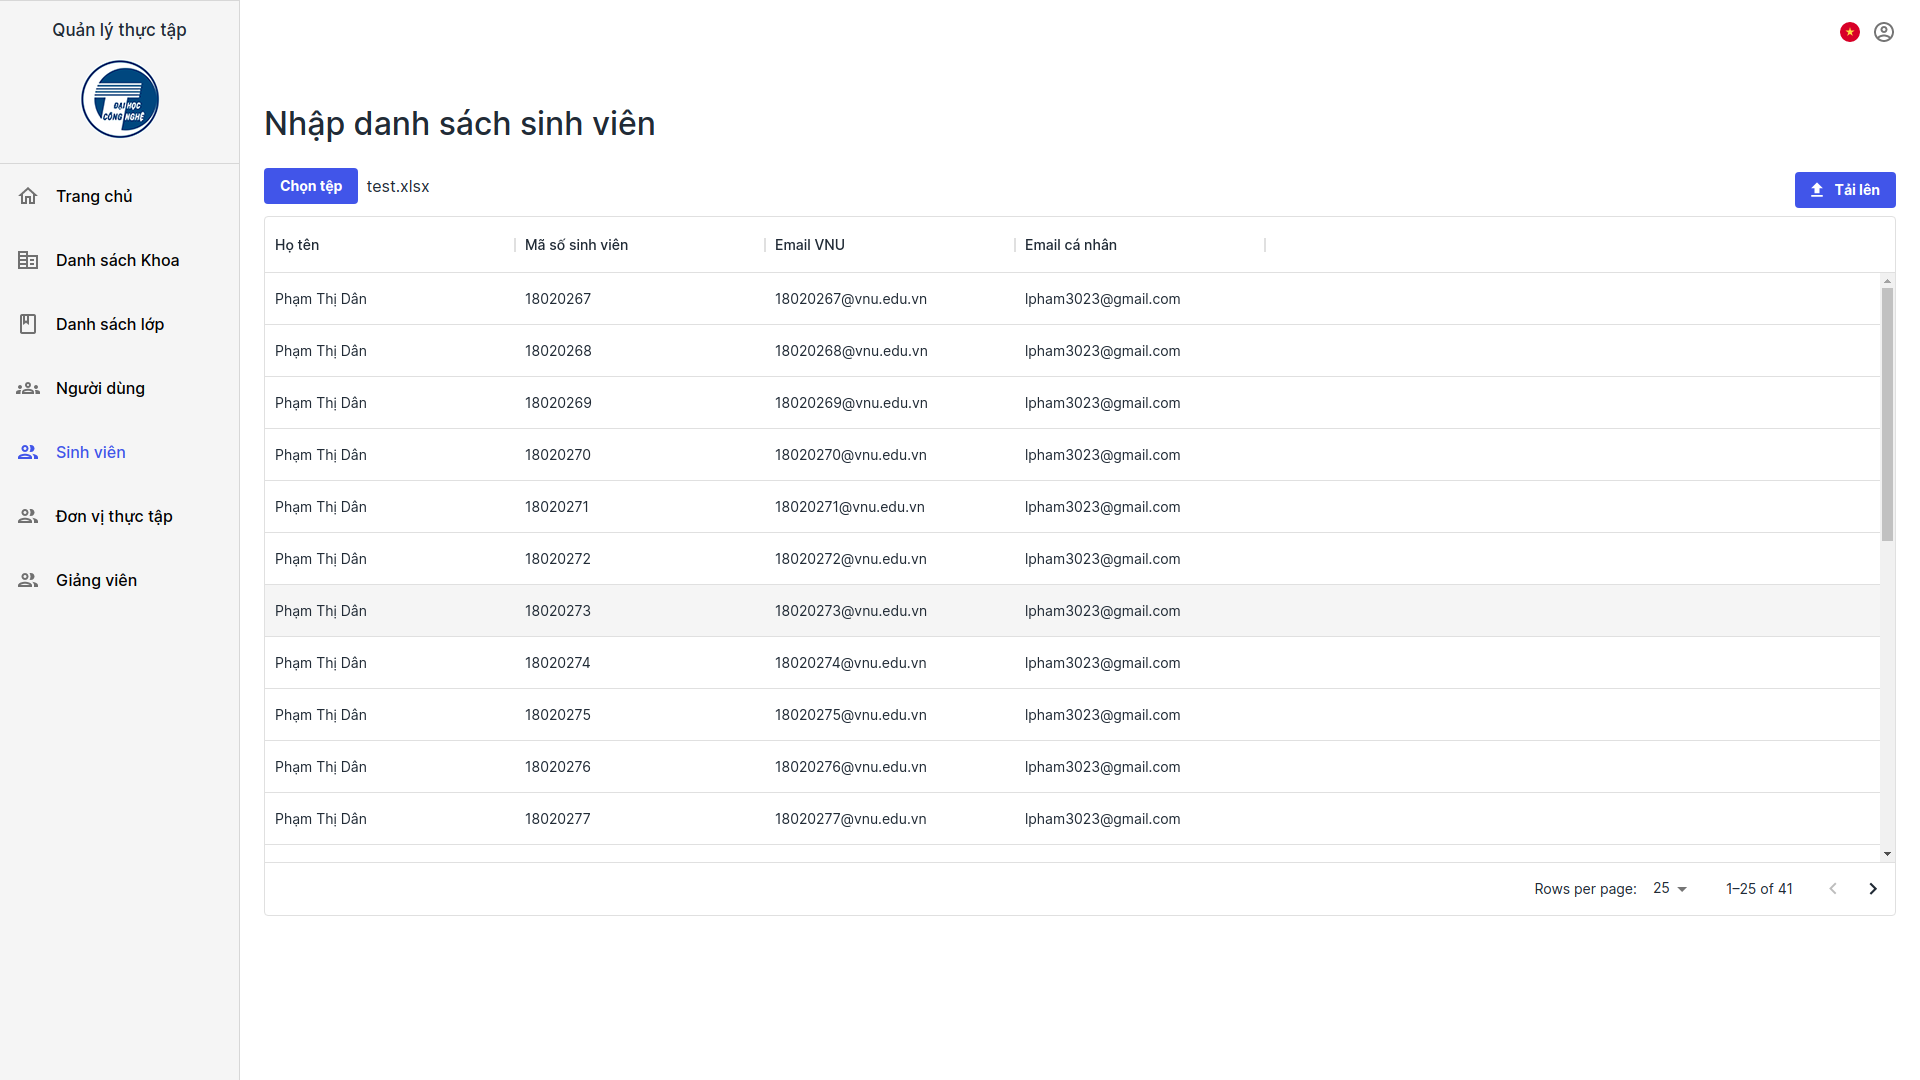
\includegraphics[width=\linewidth]{./images/image28.png}
	\caption{Luồng \emph{Quản trị viên nhập vào Danh sách sinh viên}: duyệt qua danh sách sau khi chọn tệp và tải lên danh sách}
	\label{fig:upload_list}
\end{figure}

\paragraph*{Quản trị viên đặt lại mật khẩu cho người dùng}

\begin{itemize}
	\item Hình \ref{fig:admin_access_list_users}: Quản trị viên truy cập danh sách Người dùng và chọn Đặt lại mật khẩu. 
	\item Hình \ref{fig:reset_password_success}: Đặt lại mật khẩu thành công.
\end{itemize}

\begin{figure}[]
	\includegraphics[width=\linewidth]{./images/image69.png}
	\caption{Luồng \emph{Quản trị viên đặt lại mật khẩu cho người dùng}: truy cập danh sách Người dùng và chọn Đặt lại mật khẩu}
	\label{fig:admin_access_list_users}
\end{figure}

\begin{figure}[]
	\includegraphics[width=\linewidth]{./images/image70.png}
	\caption{Luồng \emph{Quản trị viên đặt lại mật khẩu cho người dùng}: Đặt lại mật khẩu thành công}
	\label{fig:reset_password_success}
\end{figure}

\end{document}